% LaTeX file for Chapter 03














\chapter{Results}



% \begin{table}
% 
% \caption{Comparison of confidence intervals for the mean differences across scenarios. The first row of each pair corresponds to the confidence interval from the linear model (lm), while the second row corresponds to the bootstrap method.}
% \centering
% \begin{tabular}[t]{lrr}
% \toprule
%   & Lower Bound & Upper Bound\\
% \midrule
% Scenario 1 (lm) & -0.58231 & -0.54359\\
% Scenario 1 (bootstrap) & -0.58210 & -0.54355\\
% Scenario 2 (lm) & -0.59118 & -0.55371\\
% Scenario 2 (bootstrap) & -0.59091 & -0.55405\\
% Scenario 3 (lm) & -0.06784 & -0.02799\\
% \addlinespace
% Scenario 3 (bootstrap) & -0.06784 & -0.02752\\
% \bottomrule
% \end{tabular}
% \end{table}


\section{Experiment 1: TRAM-DAG (simulation)}

In this section, we present the results of the simulation study to evaluate the performance of a TRAM-DAG in a simple scenario as illustrated by the DAG in Figure \ref{fig:dag_and_matrix}. The model was fitted on synthetic data. Figure \ref{fig:exp1_loss_parameters} shows the loss and the estimated parameters for the linear shifts over epochs during training. The loss was minimized during training and the estimated parameters $\beta_{12}$ and $\beta_{13}$ converged to the true values used in the DGP. The linear shift parameters are the interpretable part of the model (log-odds ratios). 
From the fitted model, we generated samples from the observational distribution, as shown in Figure \ref{fig:exp1_observational_distribution}. The TRAM-DAG can recover the observational distribution as its samples align with the data that was used to fit the model. Then we drew samples from the interventional distribution, where $X_2 = 1$ is fixed, as shown in Figure \ref{fig:exp1_interventional_distribution}. Fixing $X_2$ leads to a distributional change in $X_3$, which was also captured by the model. The TRAM-DAG learns the linear shifts ($\beta_{12}$, $\beta_{13}$) and the complex shift $f(X_2)$, which are shown in Figure \ref{fig:exp1_shifts}. Figure~\ref{fig:exp1_intercepts} presents the intercepts learned for each of the nodes. For comparison, we added the estimated intercept functions from the Continuous Outcome Logistic Regression (Colr() function from the \texttt{tram} package \citep{hothorn2018}) for $X_1$ and $X_2$, and the true values used in the DGP for the ordinal variable $X_3$ (three cut-points for the four levels). Since the transformation functions for $X_1$ and $X_2$ contain no complex terms, they match the default form used in Colr(). Finally, Figure~\ref{fig:exp1_counterfactuals} shows the counterfactuals for $X_2$ estimated by the TRAM-DAG for varying values of $X_1$. The counterfactuals are the predicted values of $X_2$ had $X_1$ taken other values instead of the initially observed one. 

\begin{figure}[htbp]
\centering
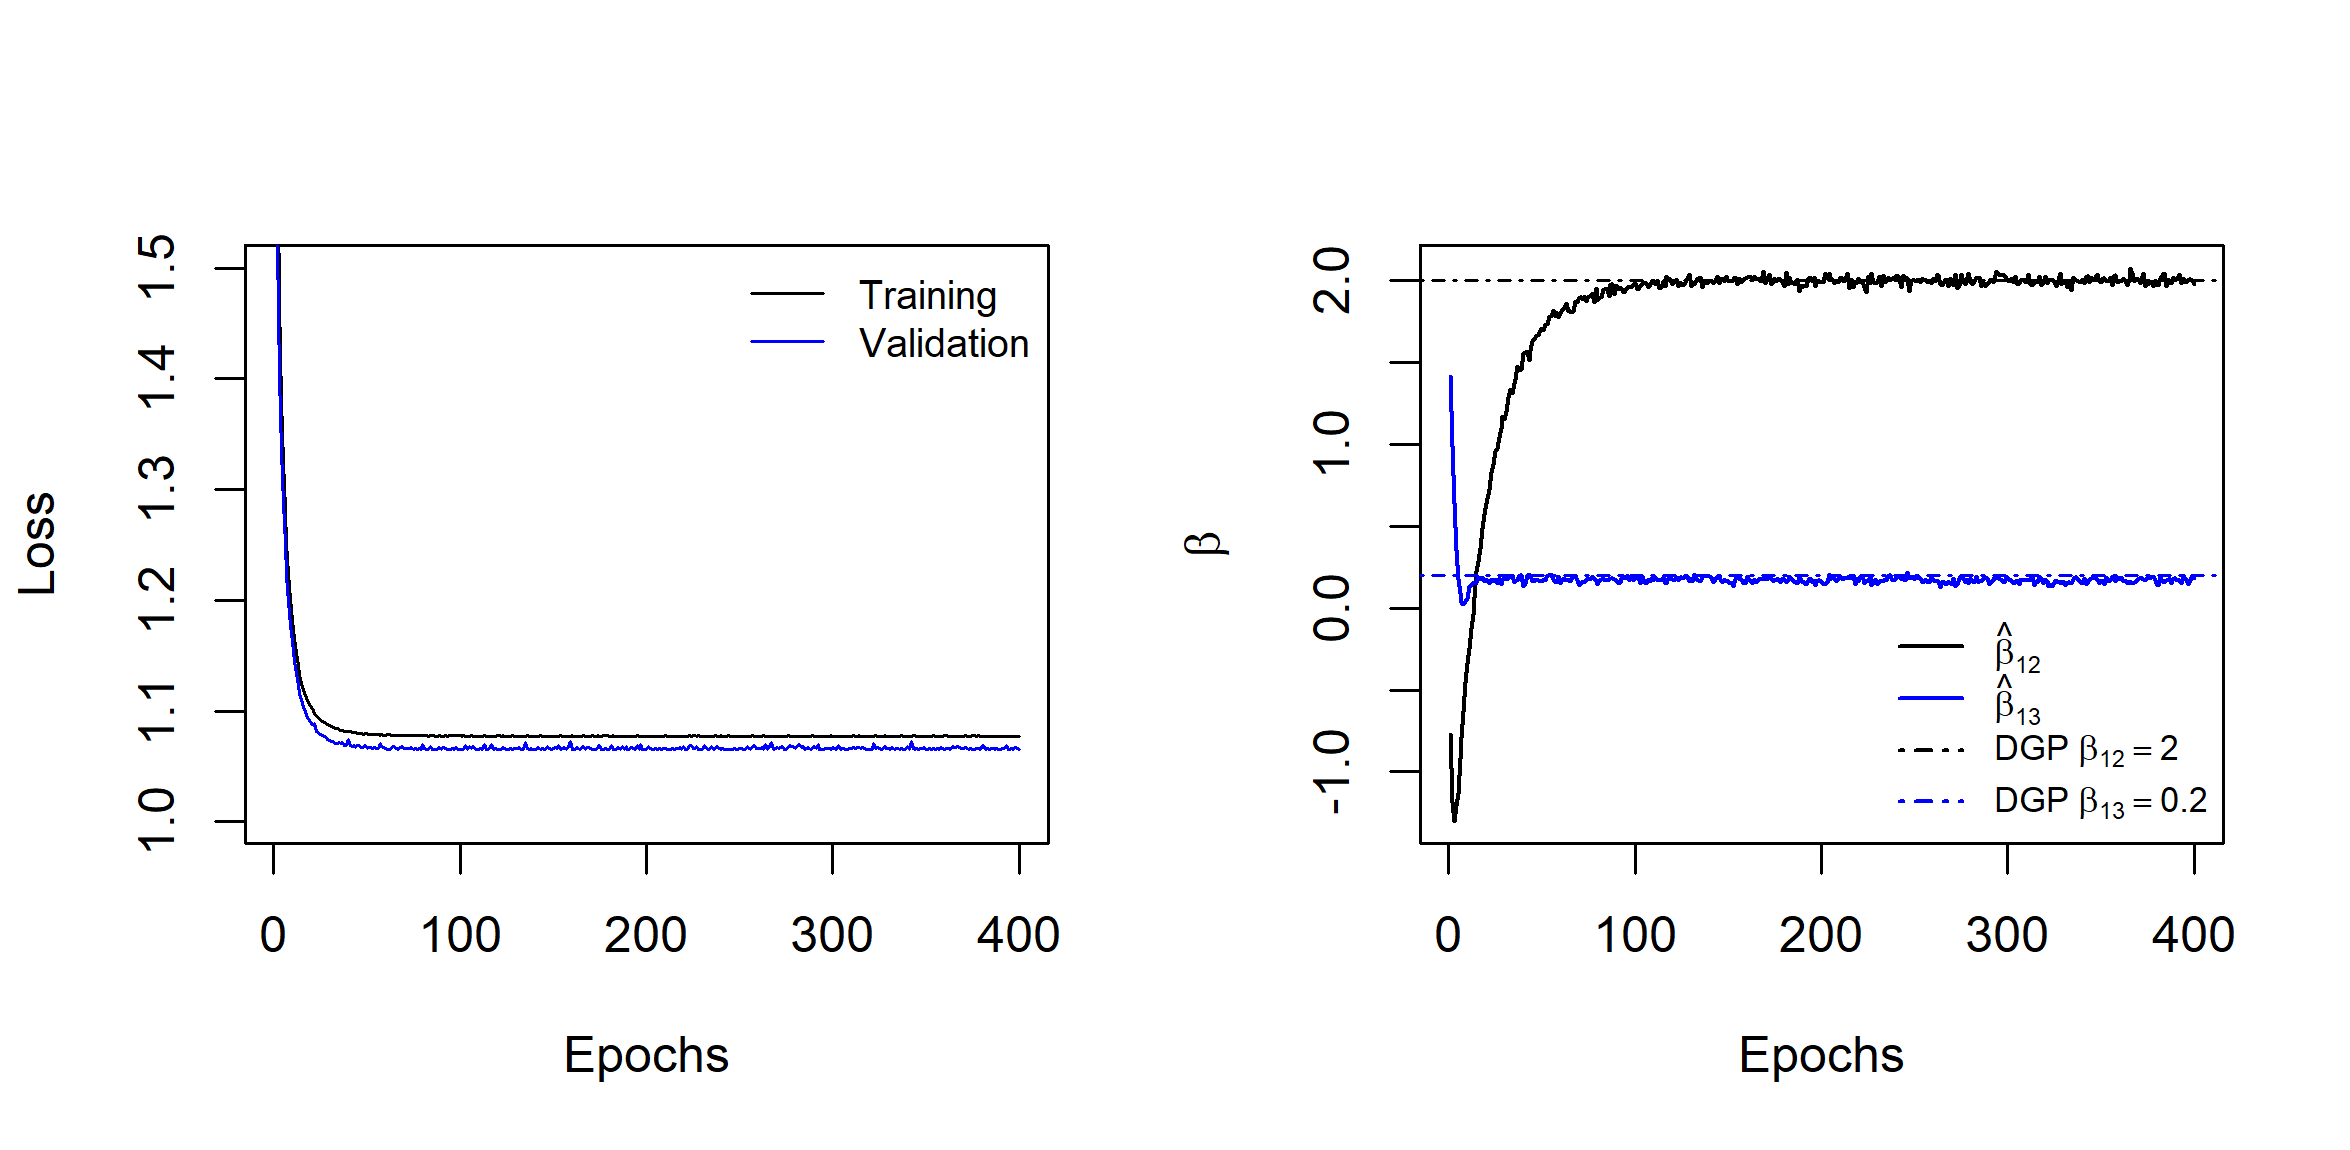
\includegraphics[width=0.9\textwidth]{img/exp1_loss_parameters.png}
\caption{TRAM-DAG model fitting over 400 epochs for Experiment 1. Left: loss functions on the training and validation sets; Right: estimated parameters (betas) for the linear shift components over epochs. The estimates converge to the true values used in the DGP.}
\label{fig:exp1_loss_parameters}
\end{figure}



\begin{figure}[htbp]
\centering
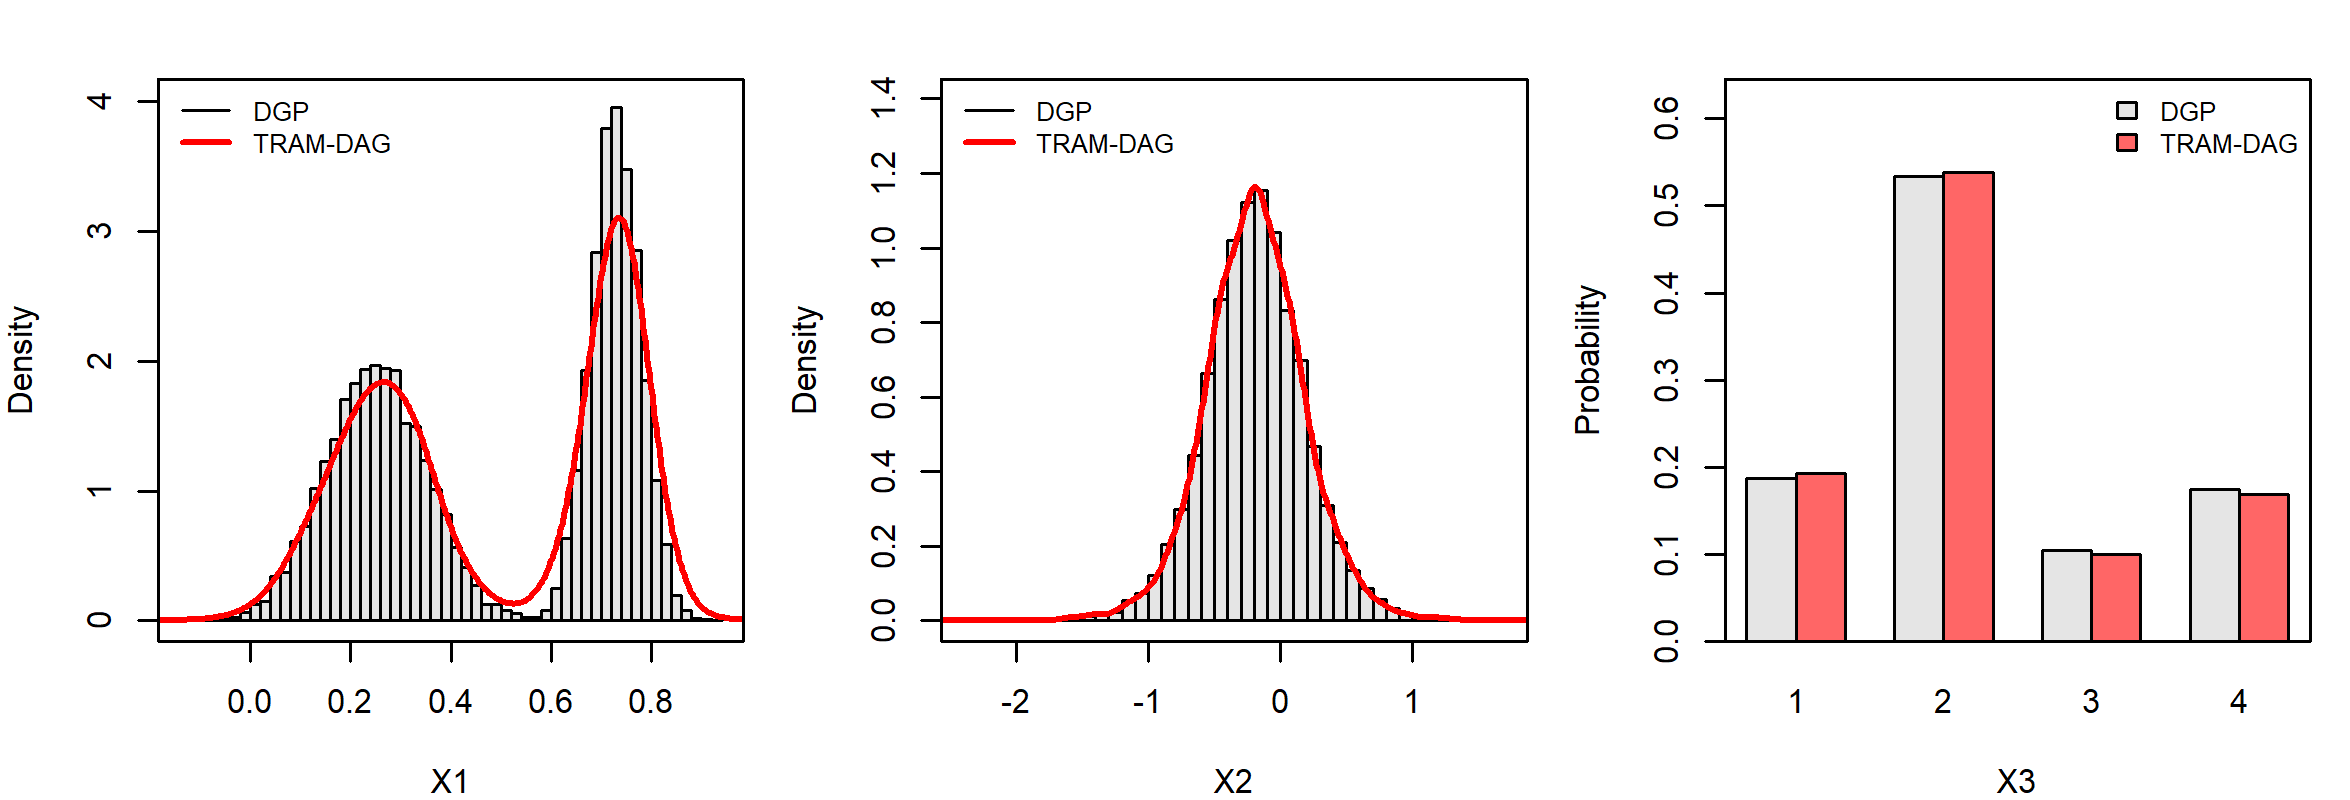
\includegraphics[width=0.9\textwidth]{img/exp1_observational_distribution.png}
\caption{Samples generated by the TRAM-DAG from the learned observational distribution, compared to the true observations from the DGP.}
\label{fig:exp1_observational_distribution}
\end{figure}




\begin{figure}[htbp]
\centering
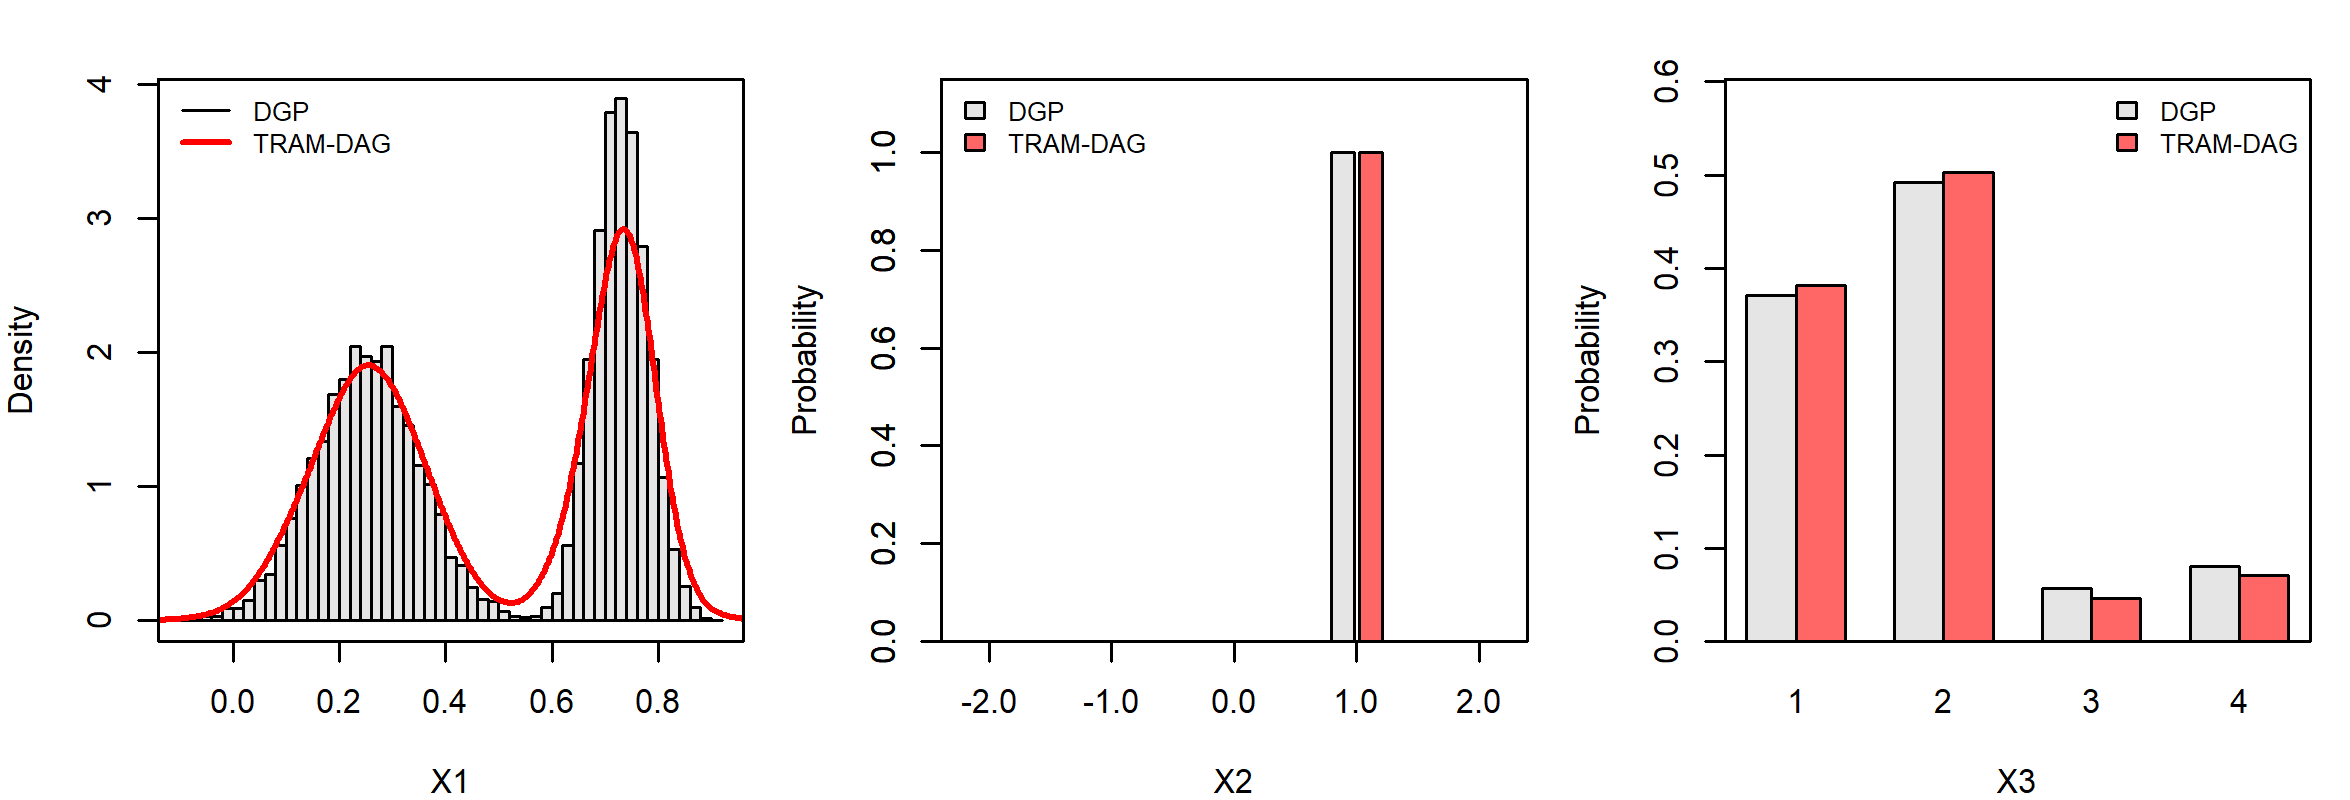
\includegraphics[width=0.9\textwidth]{img/exp1_interventional_distribution.png}
\caption{Samples generated by the TRAM-DAG compared to the true observations from the interventional distribution of the DGP, where $X_2 = 1$ is fixed. According to the DAG, this intervention induces a distributional change in $X_3$.}
\label{fig:exp1_interventional_distribution}
\end{figure}



\begin{figure}[htbp]
\centering
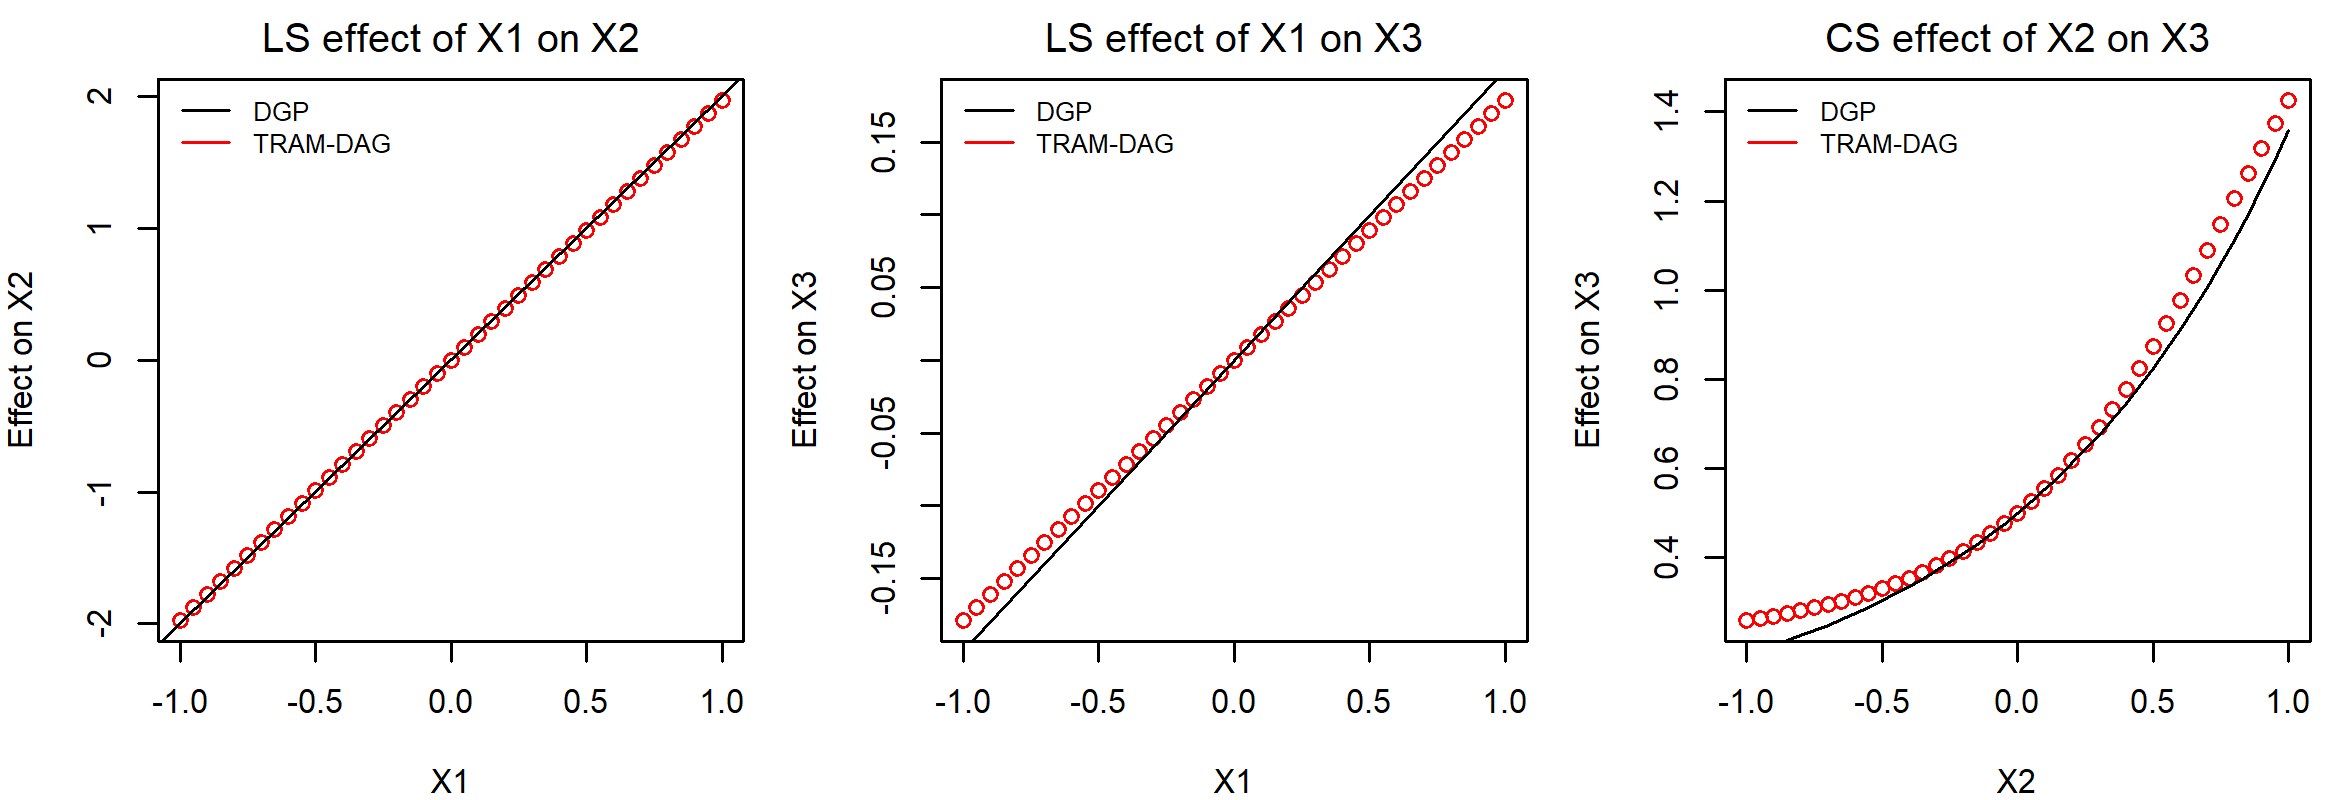
\includegraphics[width=0.9\textwidth]{img/exp1_LS_CS.png}
\caption{Linear and complex shifts learned by the TRAM-DAG. Left: LS($X_1$) on $X_2$; Middle: LS($X_1$) on $X_3$; Right: CS($X_2$) on $X_3$. For visualization, we subtracted $\delta_0 = \text{CS}(0) - f(0)$ from the estimated complex shift CS($X_2$) to align it with the true shift function $f(X_2)$ from the DGP.}
\label{fig:exp1_shifts}
\end{figure}



\begin{figure}[htbp]
\centering
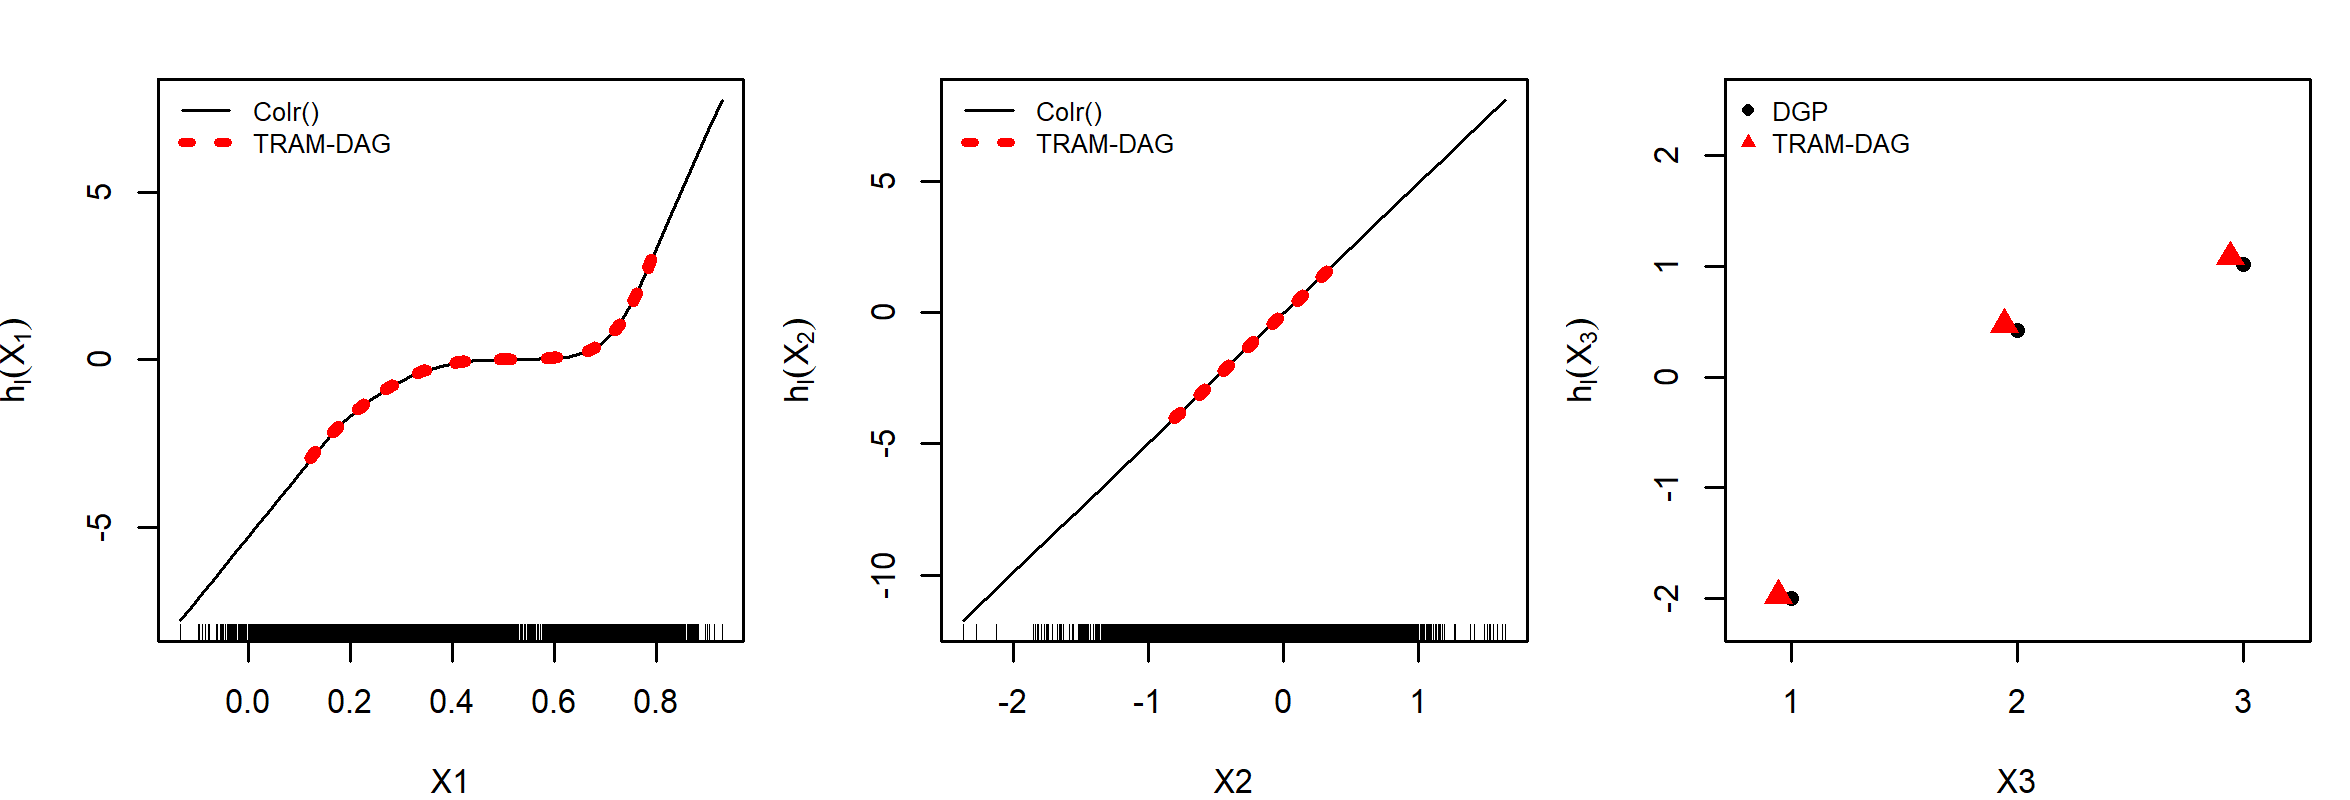
\includegraphics[width=0.9\textwidth]{img/exp1_baseline_trafo.png}
\caption{Intercepts learned for each of the nodes, along with the estimates from the \texttt{Colr()} function for the continuous variables and the true values from the DGP for the ordinal variable $X_3$. Left: Smooth baseline transformation function for continuous $X_1$; Middle: Smooth baseline transformation function for continuous $X_2$; Right: Cut-points as the baseline transformation function for ordinal $X_3$. For the last plot, we added $\delta_0 = \text{CS}(0) - f(0)$ to the estimated cut-offs to make them comparable to the true parameters from the DGP.}
\label{fig:exp1_intercepts}
\end{figure}




\begin{figure}[htbp]
\centering
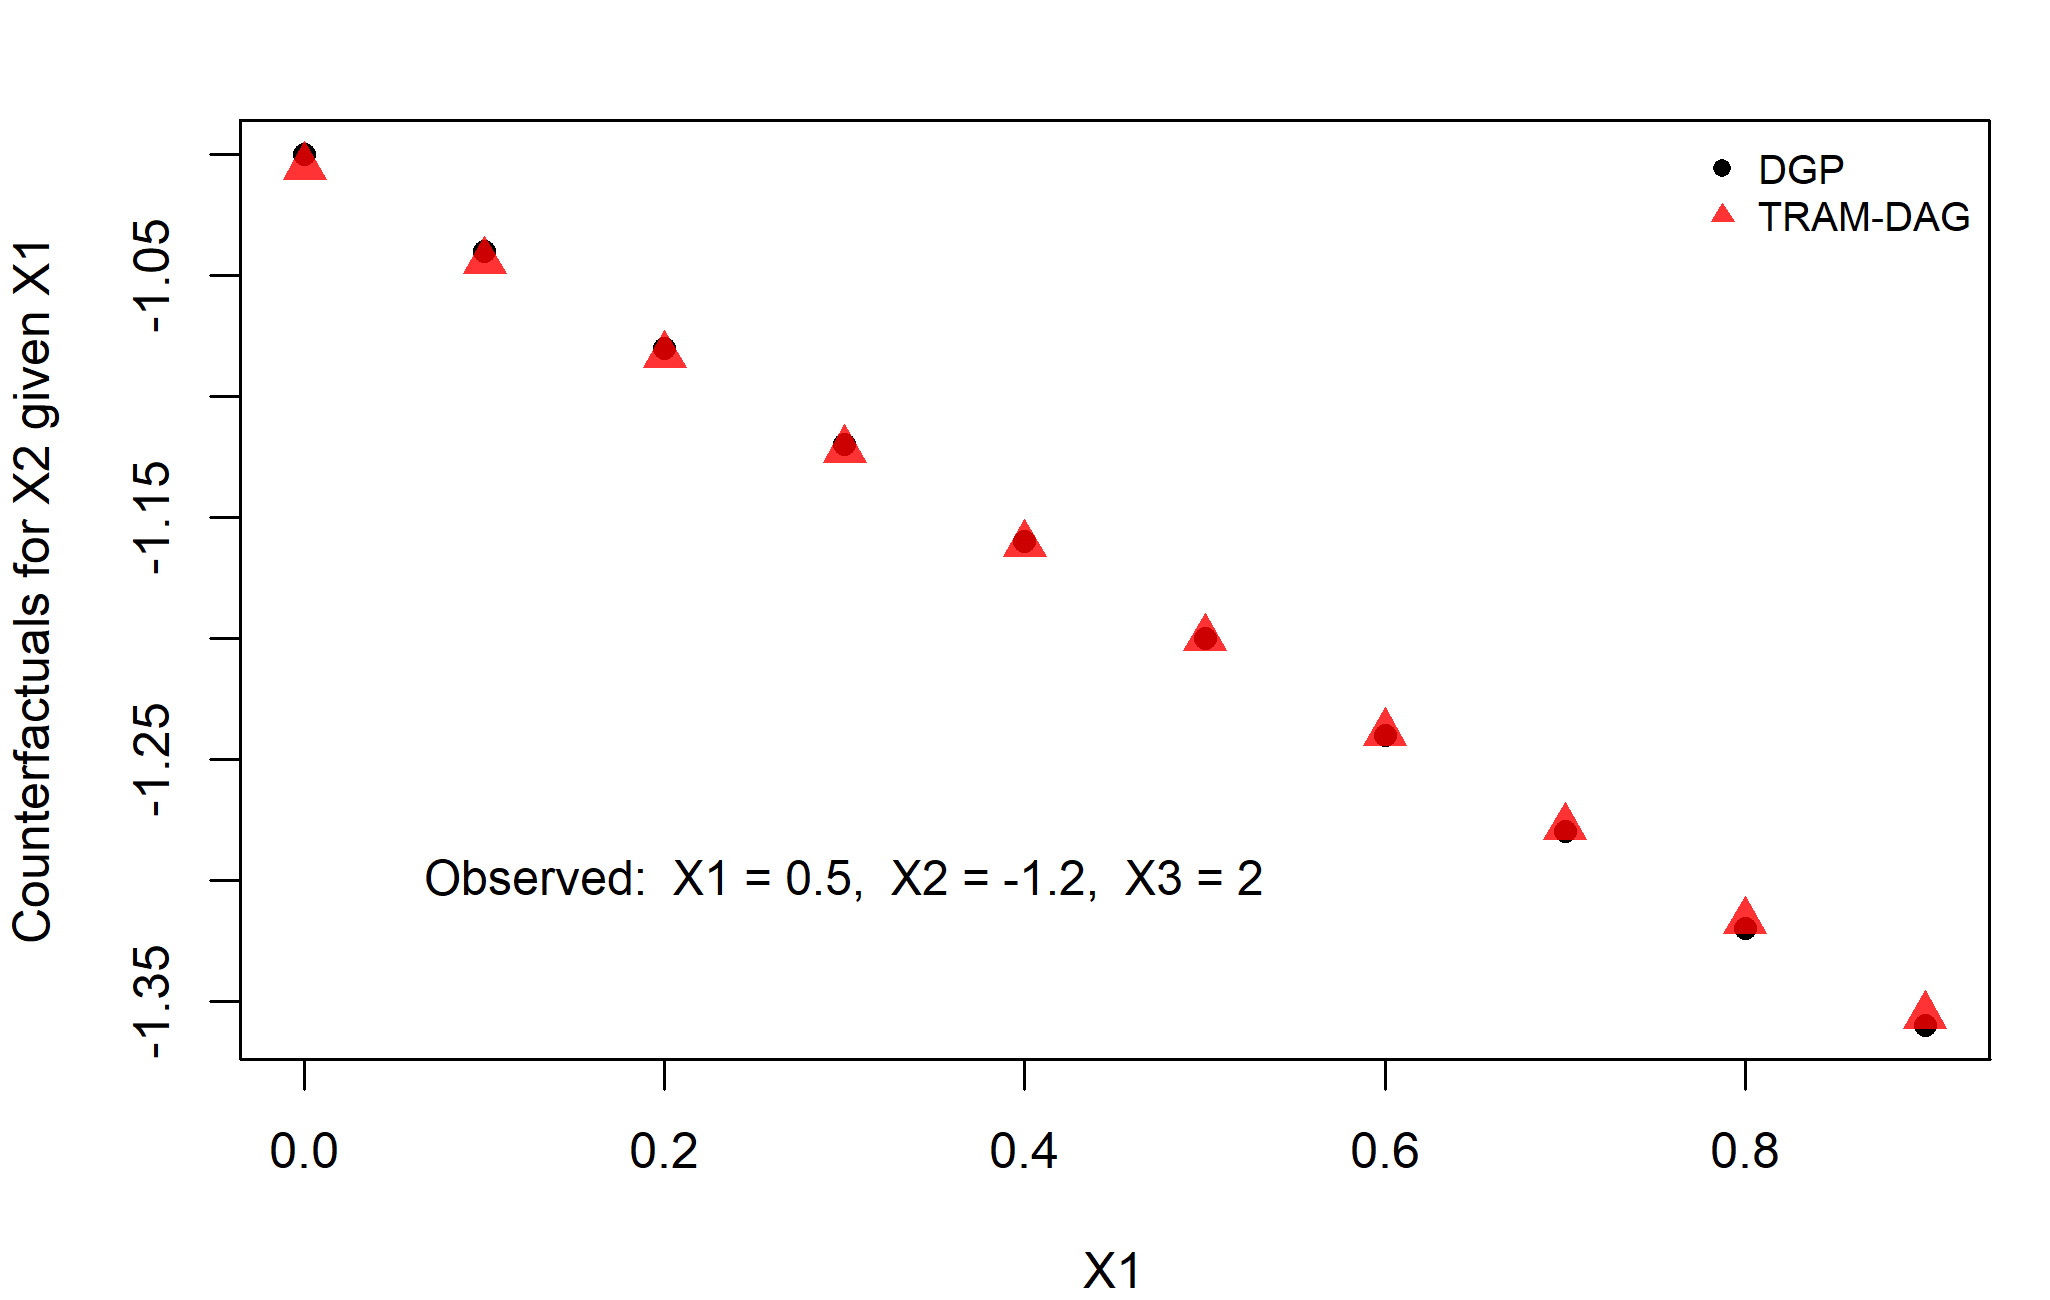
\includegraphics[width=0.9\textwidth]{img/exp1_counterfactuals.png}

\caption{Counterfactuals for $X_2$ estimated with the TRAM-DAG for varying values of $X_1$. We assumed the observed values $X_1 = 0.5$, $X_2 = -1.2$, and $X_3 = 2$, and determined the counterfactual values of $X_2$ had $X_1$ taken different values instead of the actually observed one. This illustrates how the model estimates alternative outcomes under hypothetical interventions on $X_1$.}
\label{fig:exp1_counterfactuals}
\end{figure}


\clearpage


\section{Experiment 2: ITE on International Stroke Trial (IST)} \label{sec:results_experiment2}


In this section, we present the results of the ITE estimation on the International Stroke Trial (IST) dataset. The observed treatment effect (ATE), defined as $\text{P}(Y=1|T=1) - \text{P}(Y=1|T=0)$, was -2.4\% absolute risk reduction on the training set, with a 95\% confidence interval from -4.1\% to -0.6\%. On the test set, the observed treatment effect was -0.1\%, with a 95\% confidence interval from -2.6\% to 2.3\%. The ITEs were estimated using three different models: T-learner logistic regression, T-learner tuned random forest, and S-learner TRAM-DAG. The estimated average treatment effect on the test set, calculated as $\text{ATE}_\text{pred}=\text{mean}(\text{ITE}_\text{pred})$, was -2.5\% for the T-learner logistic regression, -2.2\% for the T-learner tuned random forest, and -3.1\% for the S-learner TRAM-DAG. The density of predicted ITEs and the ITE-ATE plots for risk difference per estimated ITE subgroup, including 95\% confidence intervals, are presented in Figures \ref{fig:IST_density_ITE_ATE_glm_tlearner} - \ref{fig:IST_density_ITE_ATE_TRAM_DAG}. Calibration plots are provided in Appendix \ref{sec:calibrations_experiment2}, Figures \ref{fig:calibration_IST_glm} - \ref{fig:calibration_IST_TRAM_DAG}. 




\begin{figure}[htbp]
\centering
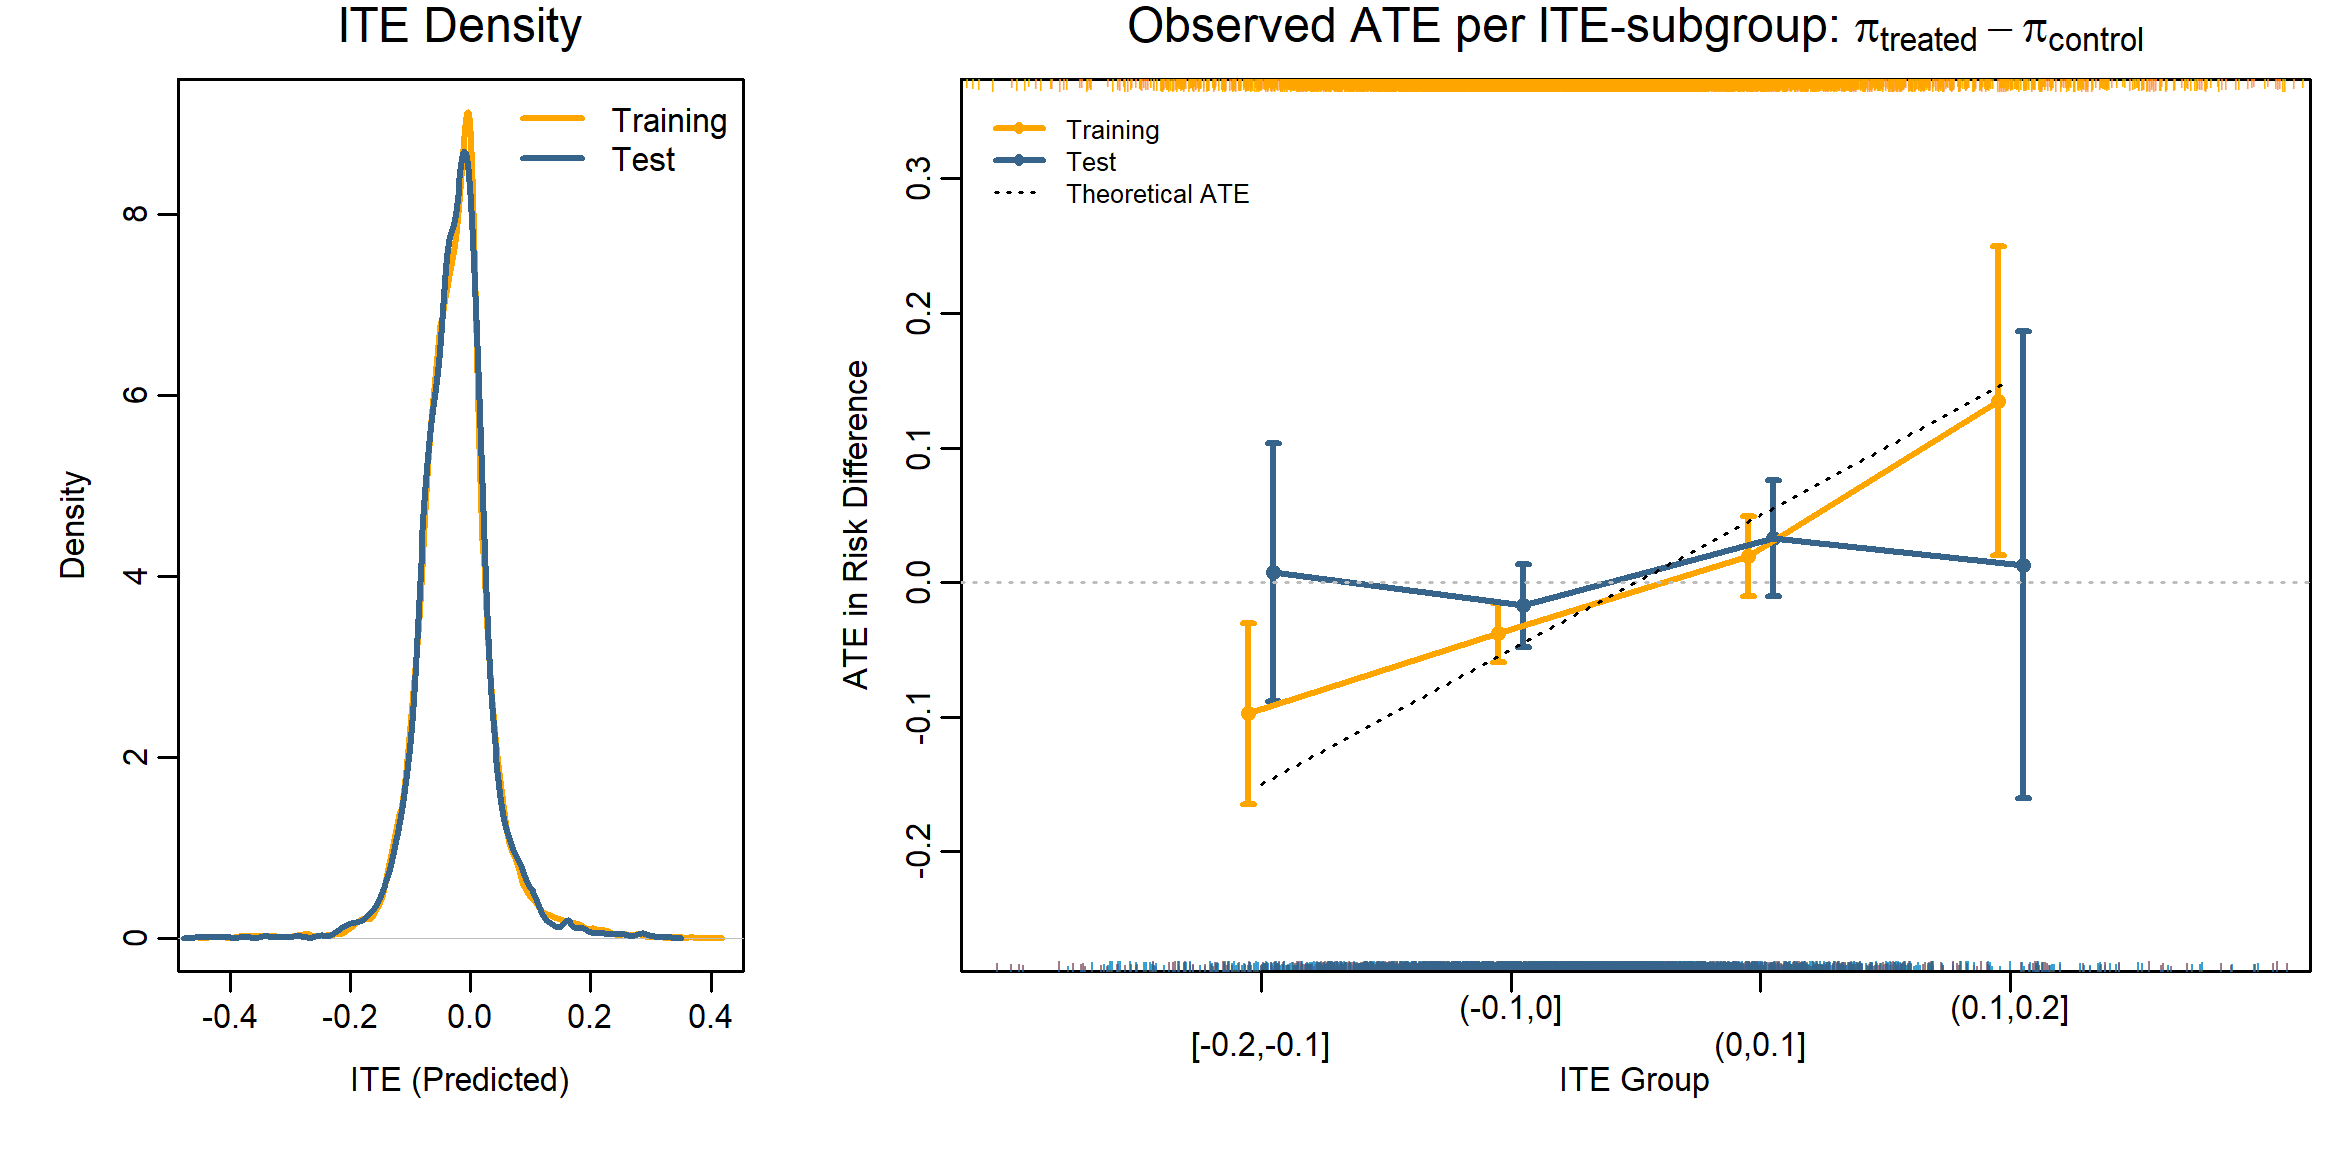
\includegraphics[width=0.9\textwidth]{img/results_IST/glm_tlearner_density_ITE_ATE.png}
\caption{Results for the International Stroke Trial (IST) using the T-learner logistic regression. Left: density of predicted ITEs in the training and test sets; Right: observed ATE in terms of risk difference per estimated ITE subgroup.}
\label{fig:IST_density_ITE_ATE_glm_tlearner}
\end{figure}



\begin{figure}[htbp]
\centering
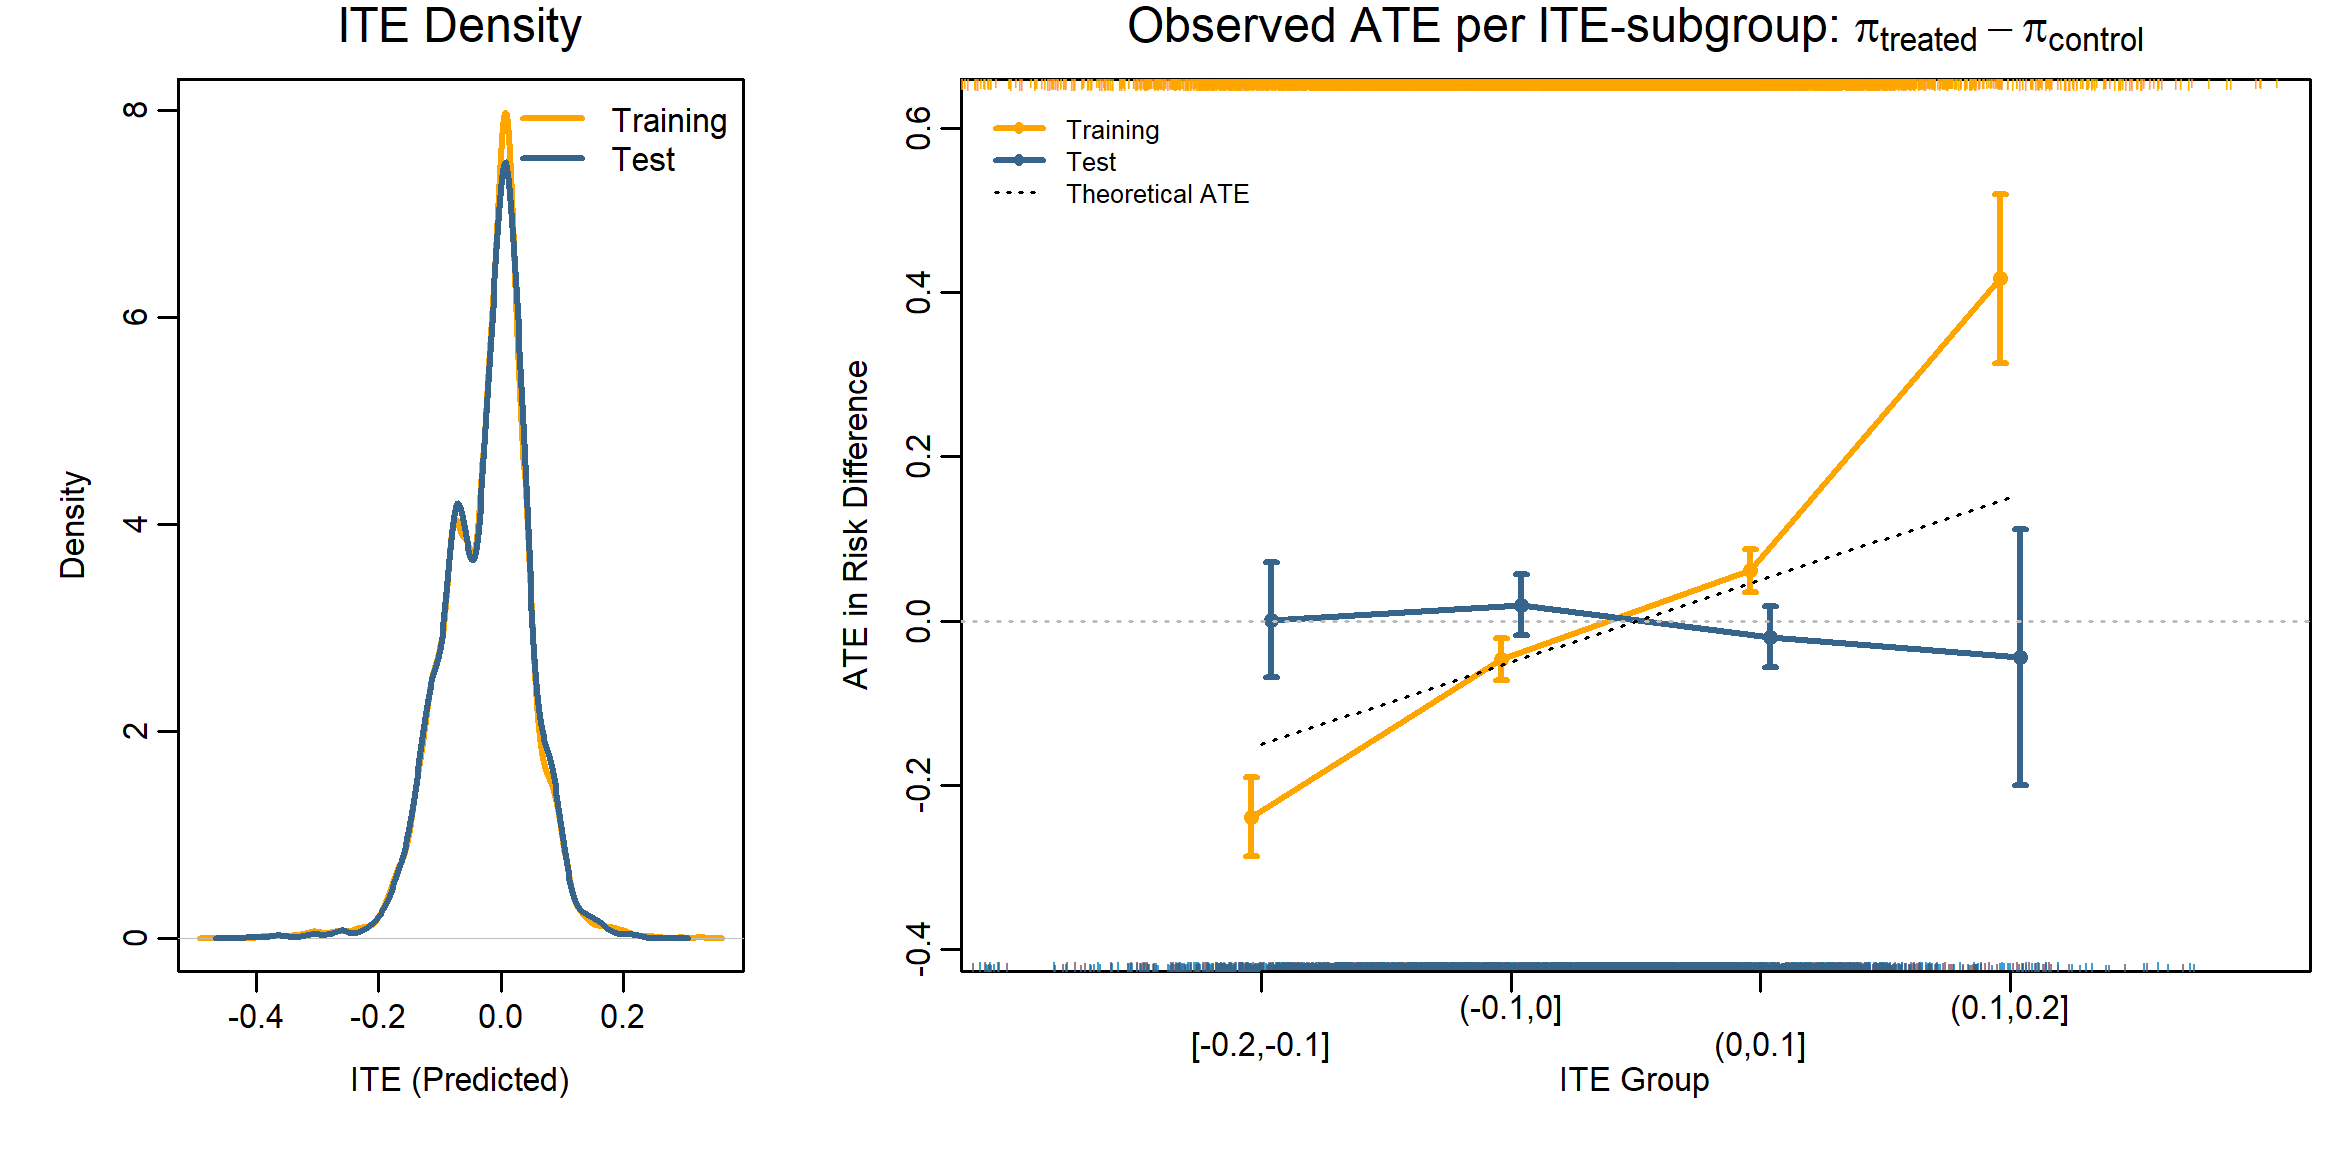
\includegraphics[width=0.9\textwidth]{img/results_IST/IST_tuned_rf_tlearner_density_ITE_ATE.png}
\caption{Results for the International Stroke Trial (IST) using the T-learner tuned random forest. Left: density of predicted ITEs in the training and test sets; Right: observed ATE in terms of risk difference per estimated ITE subgroup.}
\label{fig:IST_density_ITE_ATE_tuned_rf}
\end{figure}


\begin{figure}[htbp]
\centering
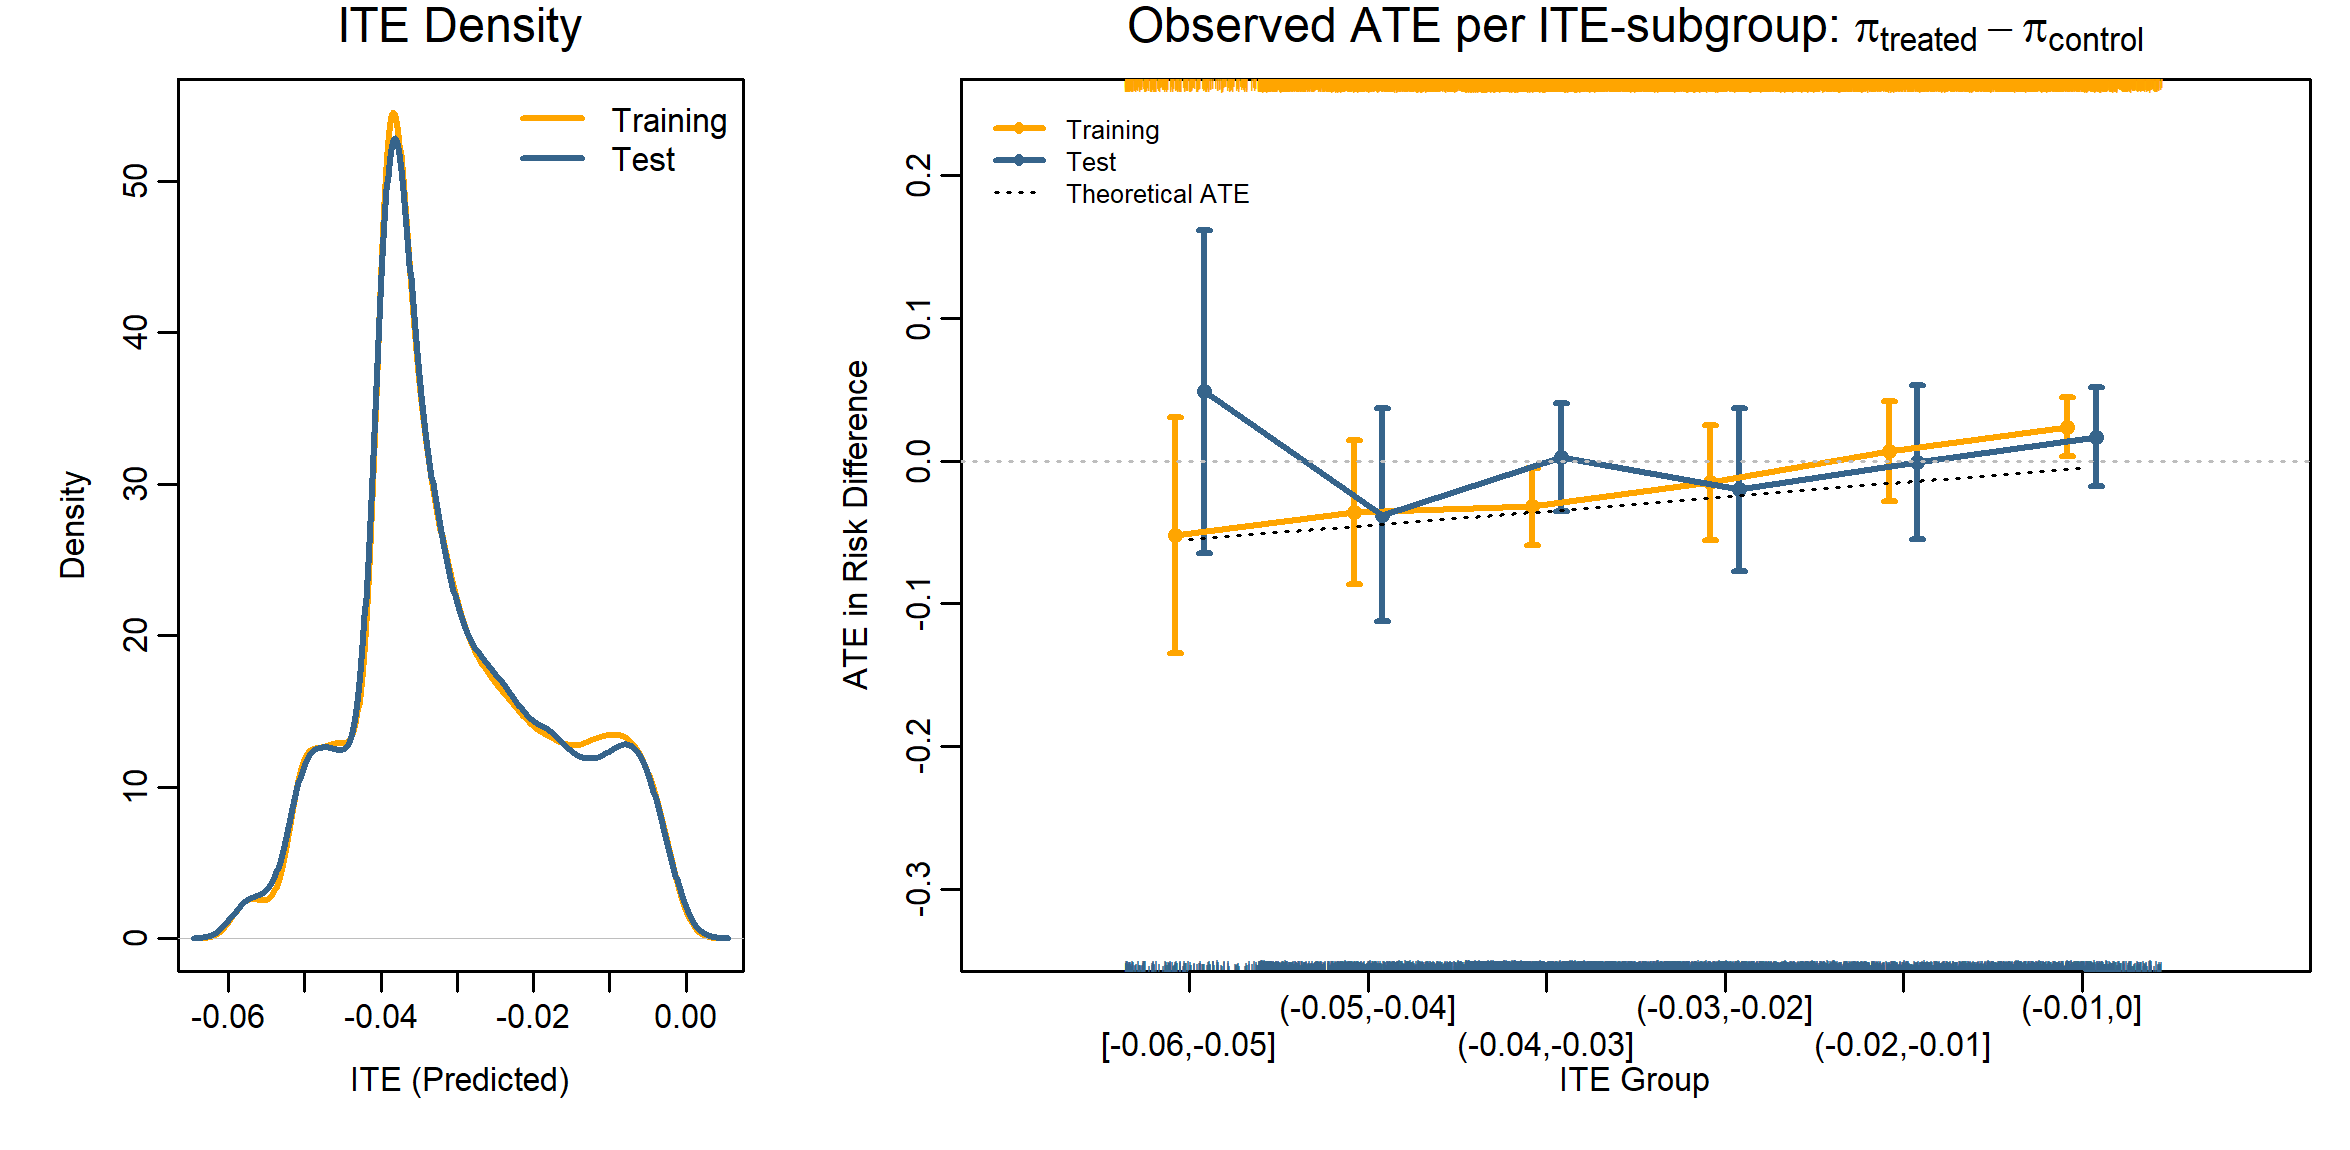
\includegraphics[width=0.9\textwidth]{img/results_IST/IST_TRAM_DAG_slearner_density_ITE_ATE.png}
\caption{Results for the International Stroke Trial (IST) using the S-learner TRAM-DAG. Left: density of predicted ITEs in the training and test sets; Right: observed ATE in terms of risk difference per estimated ITE subgroup.}
\label{fig:IST_density_ITE_ATE_TRAM_DAG}
\end{figure}



\clearpage

 

\section{Experiment 3: ITE model robustness in RCTs (simulation)} \label{sec:results_experiment3}

In this section, we present the performance of two causal ML models for estimating the ITE under different simulated scenarios. Scenario 1 represents the ideal case where all variables are observed and treatment effects and heterogeneity are large. Scenario 2 uses the same DGP as in Scenario 1 but removes the covariate $X_1$, which has a strong interaction effect with the treatment, from the dataset and treats it as unobserved. Finally, in Scenario 3, the coefficients for the direct and interaction treatment effects are reduced, resulting in low heterogeneity. All variables are observed again in this last scenario. 

In each scenario, we applied the T-learner logistic regression and the T-learner tuned random forest. The results of the models for the three scenarios are presented in Figures~\ref{fig:fully_observed_glm_tlearner} to~\ref{fig:small_interaction_tuned_rf_tlearner}.


\subsection{Scenario (1): Fully observed, large effects}



\begin{figure}[htbp]
\centering
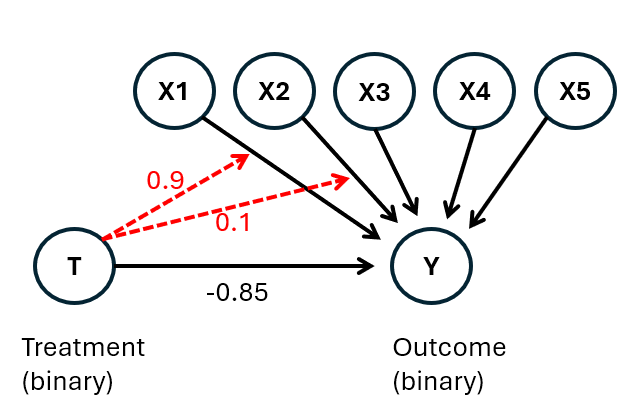
\includegraphics[width=0.35\textwidth]{img/results_ITE_simulation/simulation_observed.png}
\caption{DAG for Scenario~(1), where all variables are observed and both treatment and interaction effects are strong. The numbers indicate the coefficients on the log-odds scale. Red arrows represent interaction effects between treatment ($T$) and covariates ($X_1$ and $X_2$) on the outcome ($Y$).}
\label{fig:fully_observed_dag}
\end{figure}


\begin{figure}[htbp]
\centering
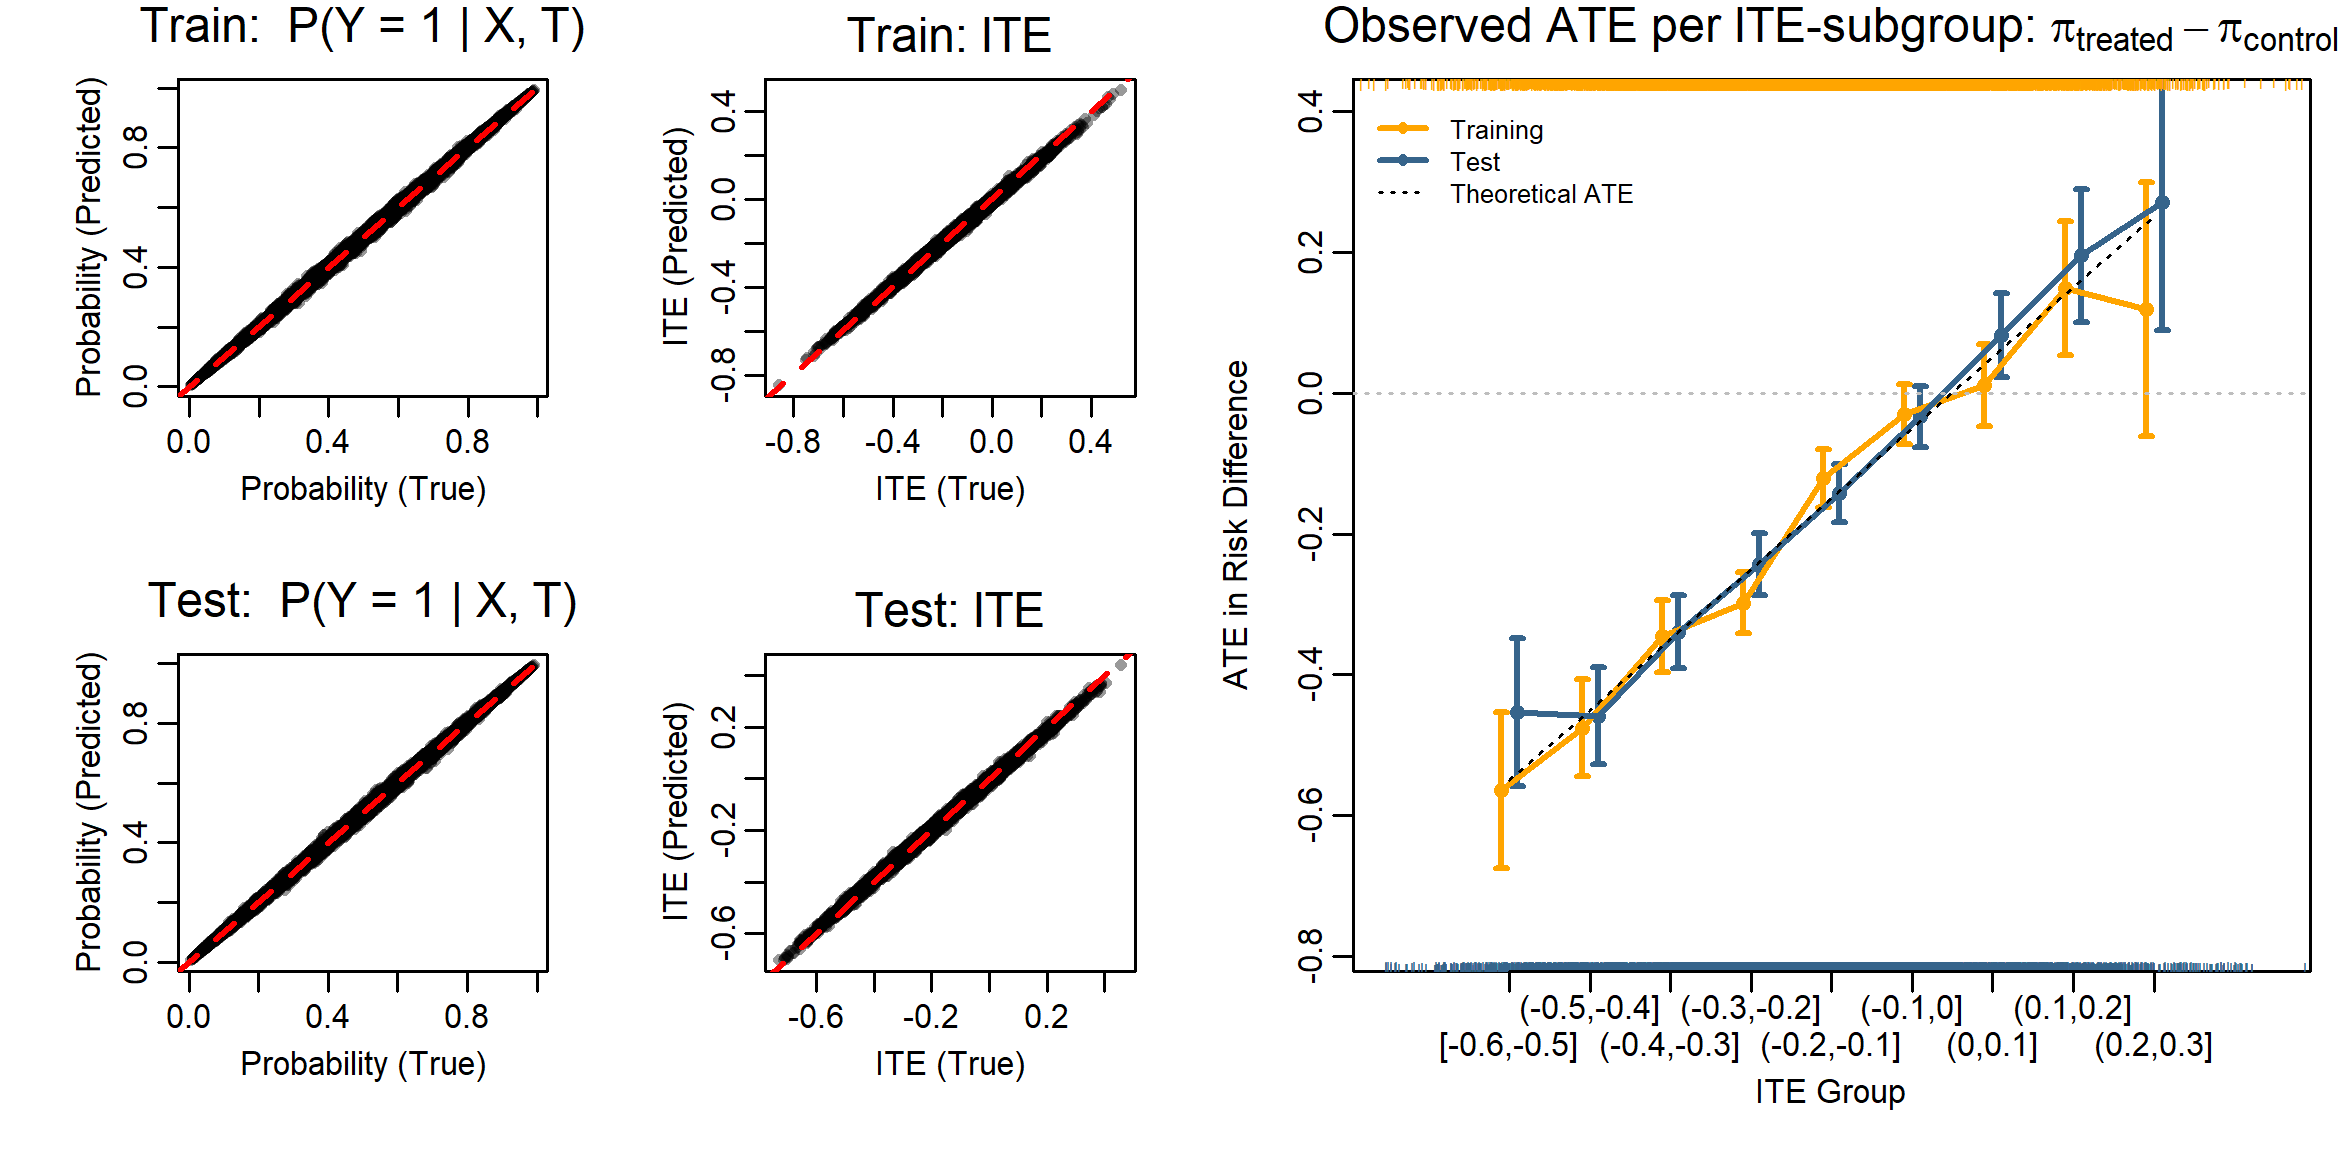
\includegraphics[width=0.9\textwidth]{img/results_ITE_simulation/fully_observed_glm_tlearner.png}
\caption{Results of the T-learner logistic regression in Scenario~(1), where the DAG is fully observed and both treatment and interaction effects are strong. Left: true vs. predicted probabilities for $\text{P}(Y = 1 \mid X, T)$; Middle: true vs. predicted ITEs; Right: observed ATE in terms of risk difference per estimated ITE subgroup.}
\label{fig:fully_observed_glm_tlearner}
\end{figure}


\begin{figure}[htbp]
\centering
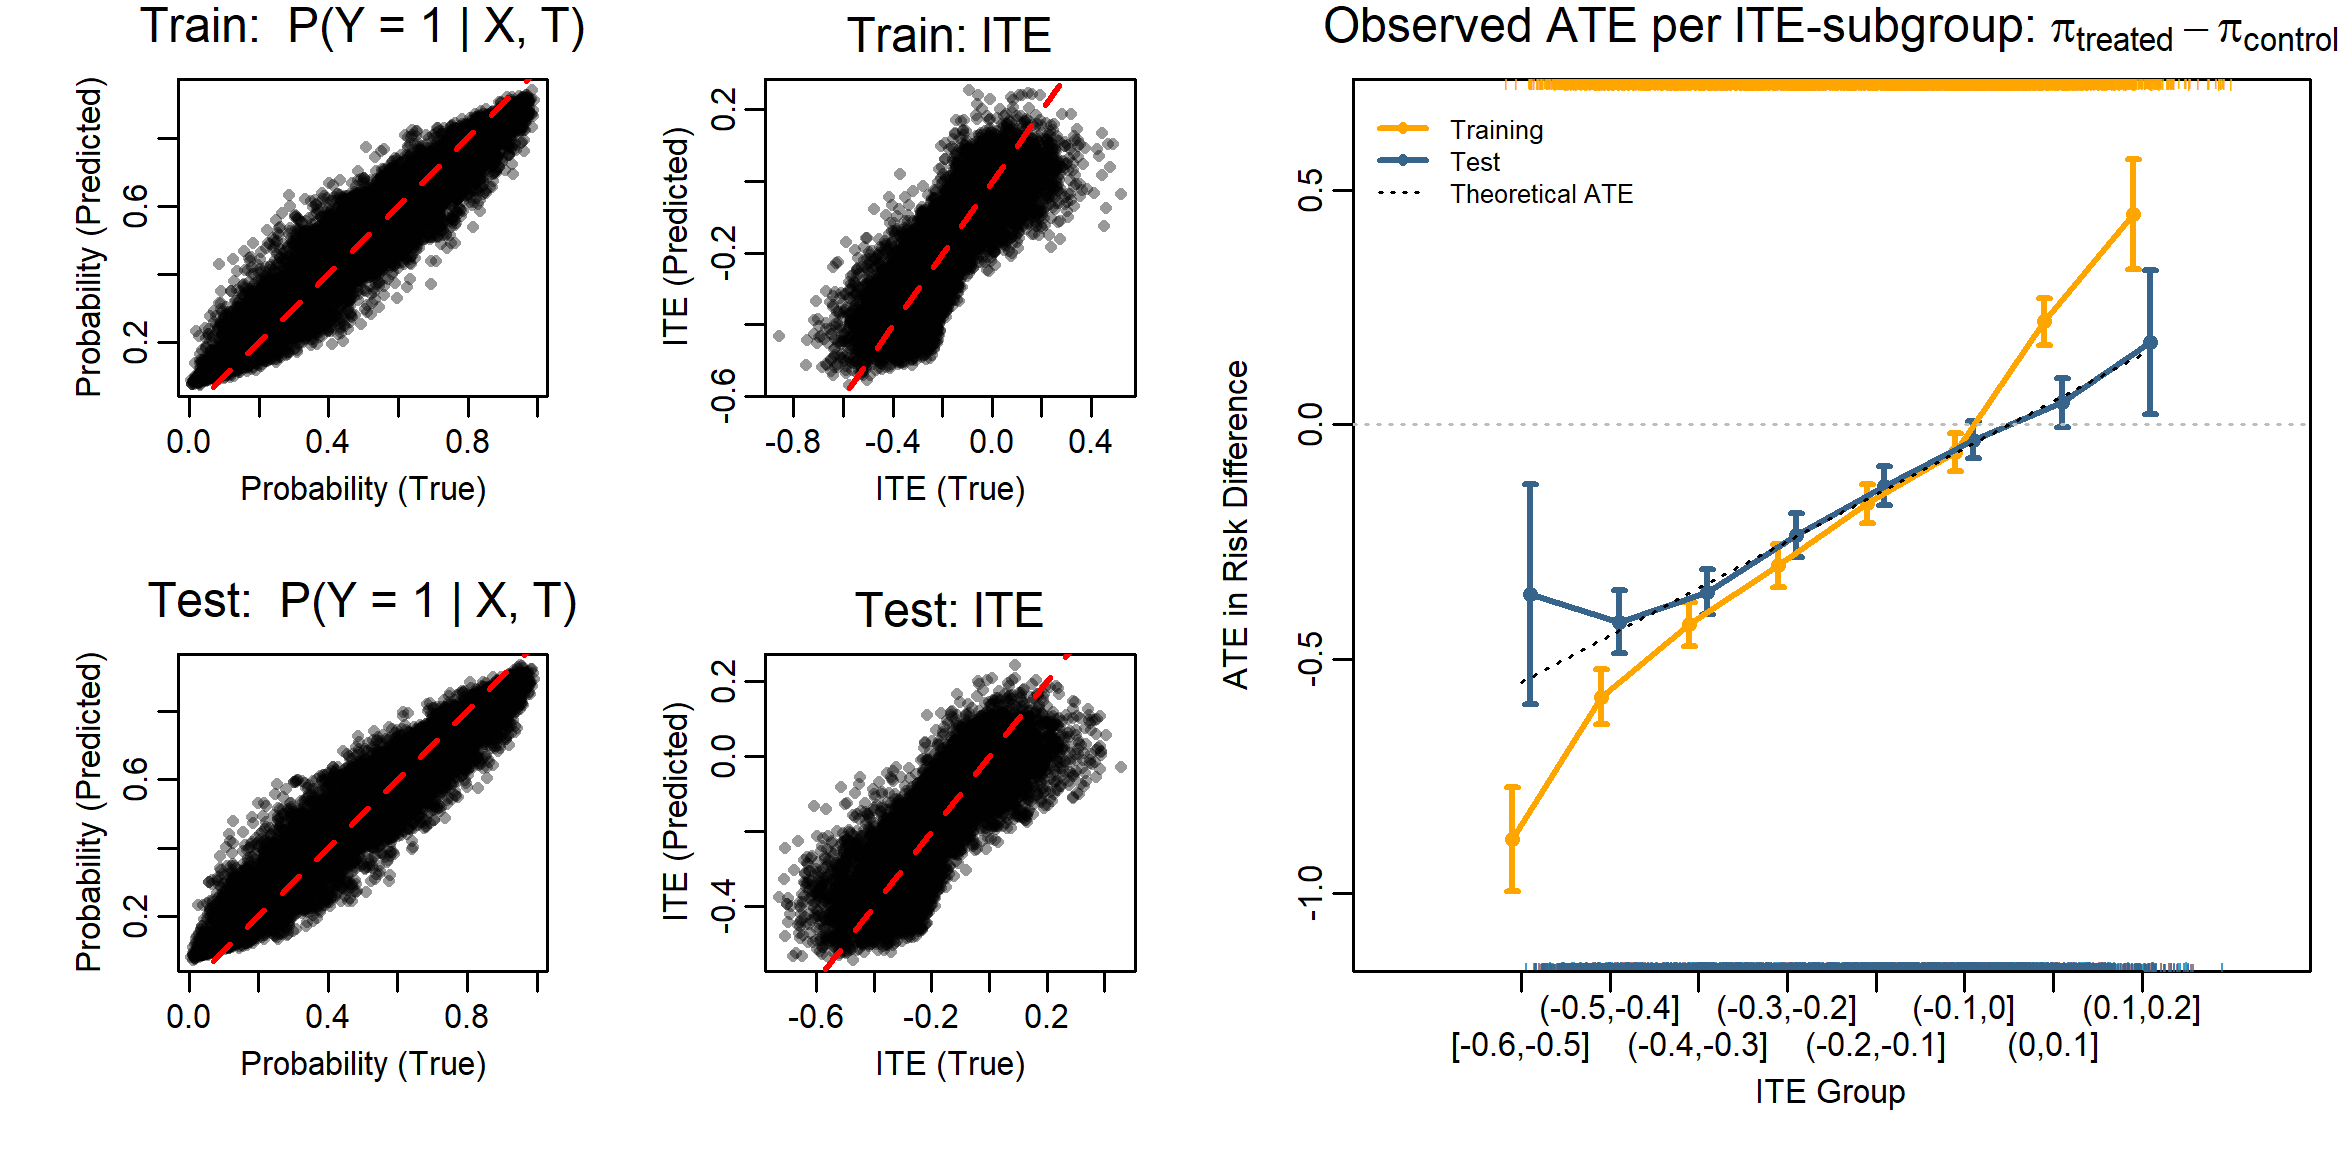
\includegraphics[width=0.9\textwidth]{img/results_ITE_simulation/fully_observed_tuned_rf_tlearner.png}
\caption{Results of the T-learner tuned random forest in Scenario~(1), where the DAG is fully observed and both treatment and interaction effects are strong. Left: true vs. predicted probabilities for $\text{P}(Y = 1 \mid X, T)$; Middle: true vs. predicted ITEs; Right: observed ATE in terms of risk difference per estimated ITE subgroup.}
\label{fig:fully_tuned_rf_tlearner}
\end{figure}


\clearpage



\subsection{Scenario (2): Unobserved interaction}

\begin{figure}[htbp]
\centering
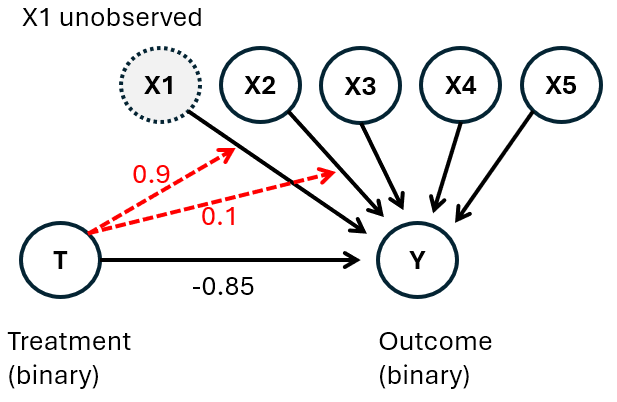
\includegraphics[width=0.35\textwidth]{img/results_ITE_simulation/simulation_unobserved.png}
\caption{DAG for Scenario~(2), where there are strong treatment and interaction effects, but variable $X_1$ is not observed. The numbers indicate the coefficients on the log-odds scale. Red arrows represent interaction effects between treatment ($T$) and covariates ($X_1$ and $X_2$) on the outcome ($Y$).}
\label{fig:unobserved_interaction_dag}
\end{figure}



\begin{figure}[htbp]
\centering
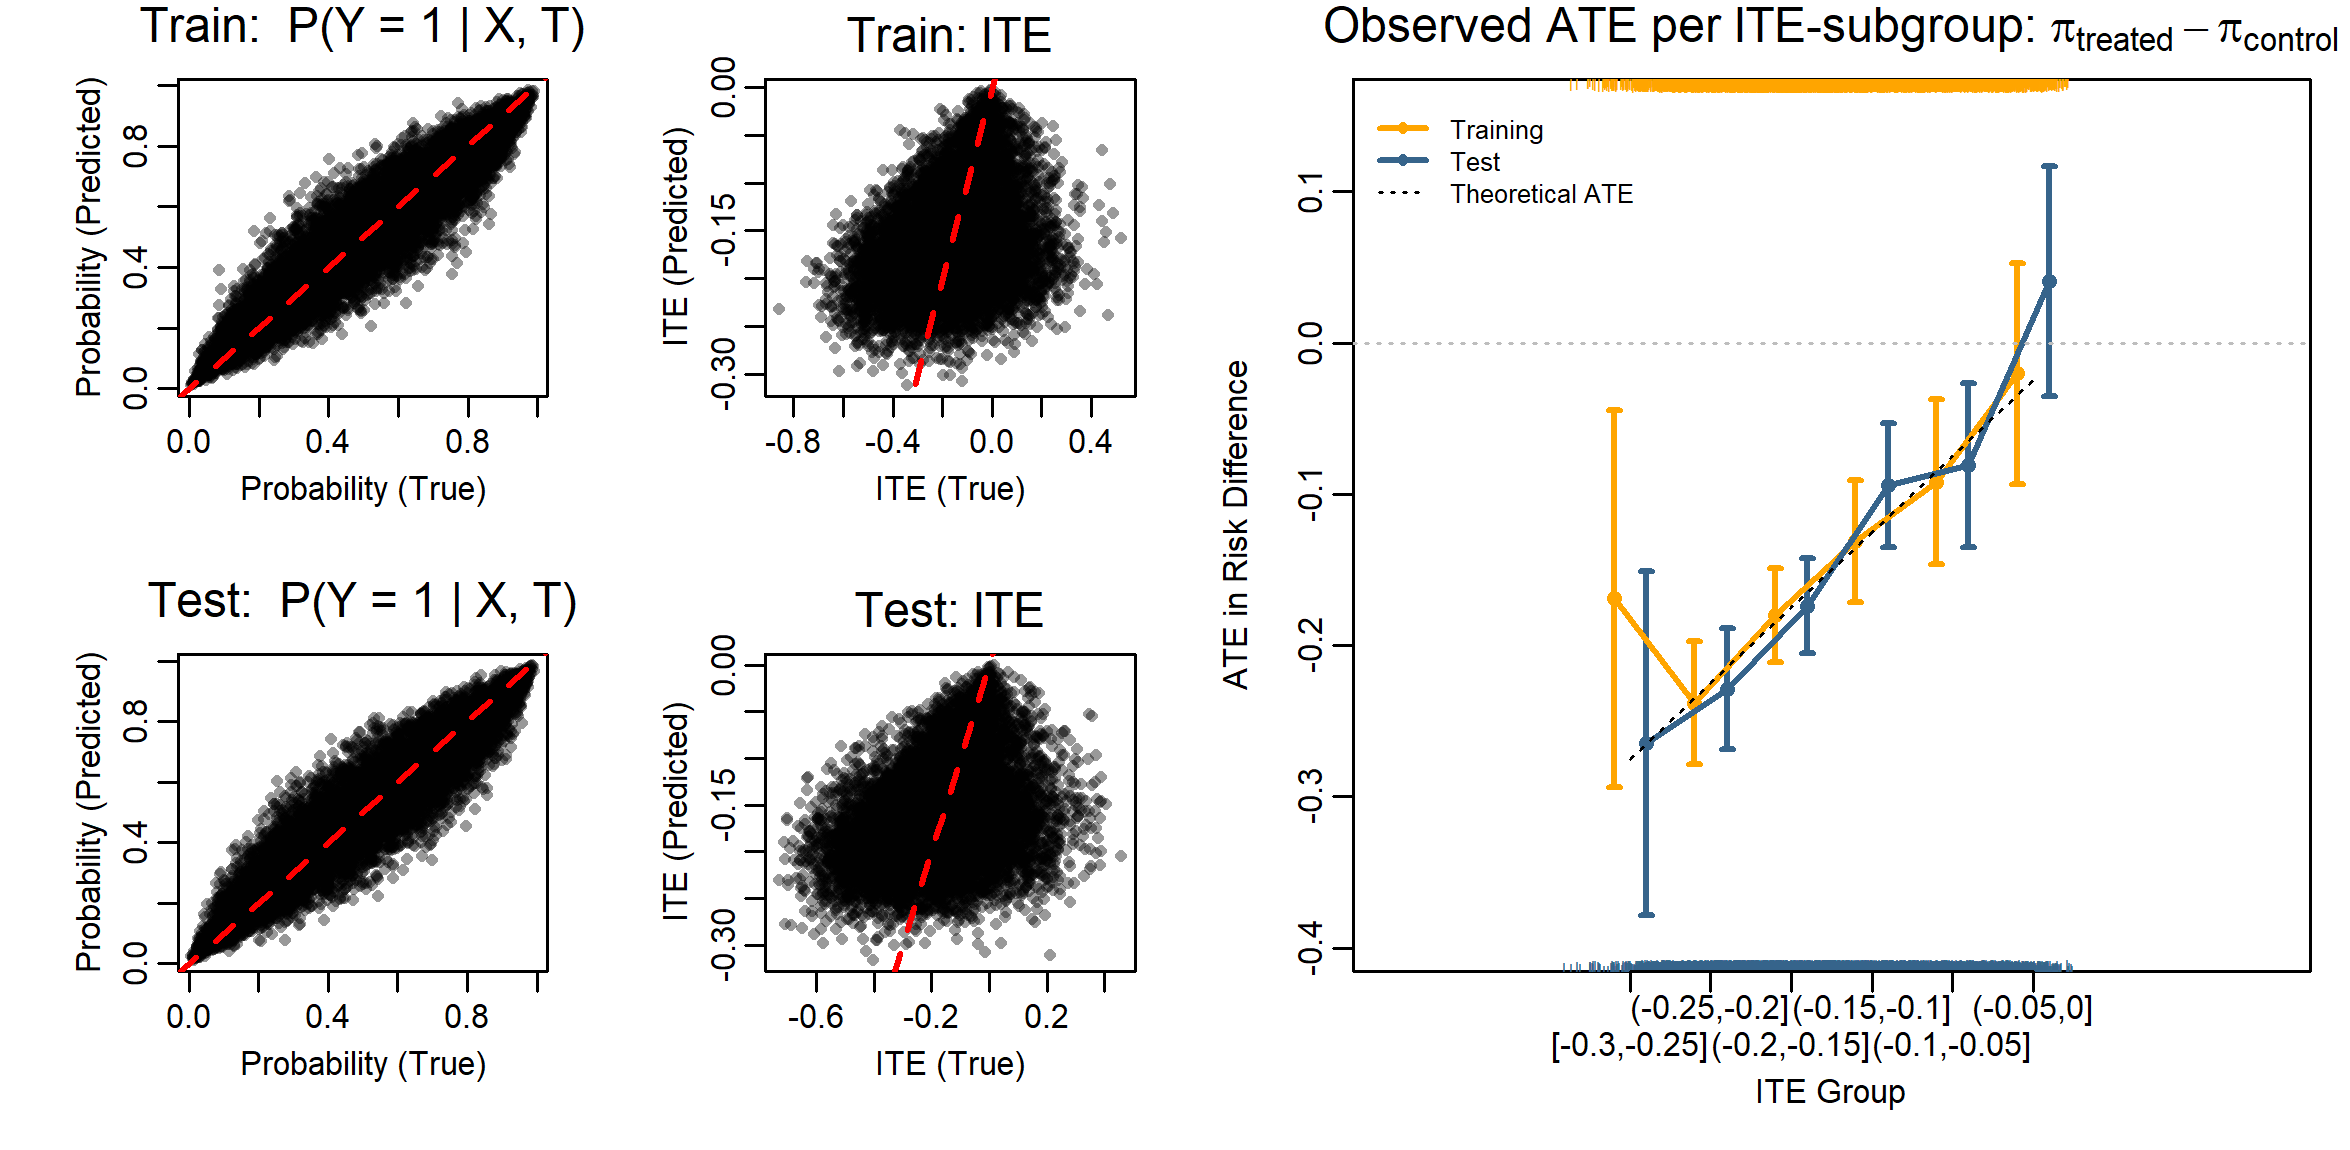
\includegraphics[width=0.9\textwidth]{img/results_ITE_simulation/unobserved_interaction_glm_tlearner.png}
\caption{Results of the T-learner logistic regression in Scenario~(2), where there are strong treatment and interaction effects, but variable $X_1$ is not observed. Left: true vs. predicted probabilities for $\text{P}(Y = 1 \mid X, T)$; Middle: true vs. predicted ITEs; Right: observed ATE in terms of risk difference per estimated ITE subgroup.}
\label{fig:unobserved_interaction_glm_tlearner}
\end{figure}



\begin{figure}[htbp]
\centering
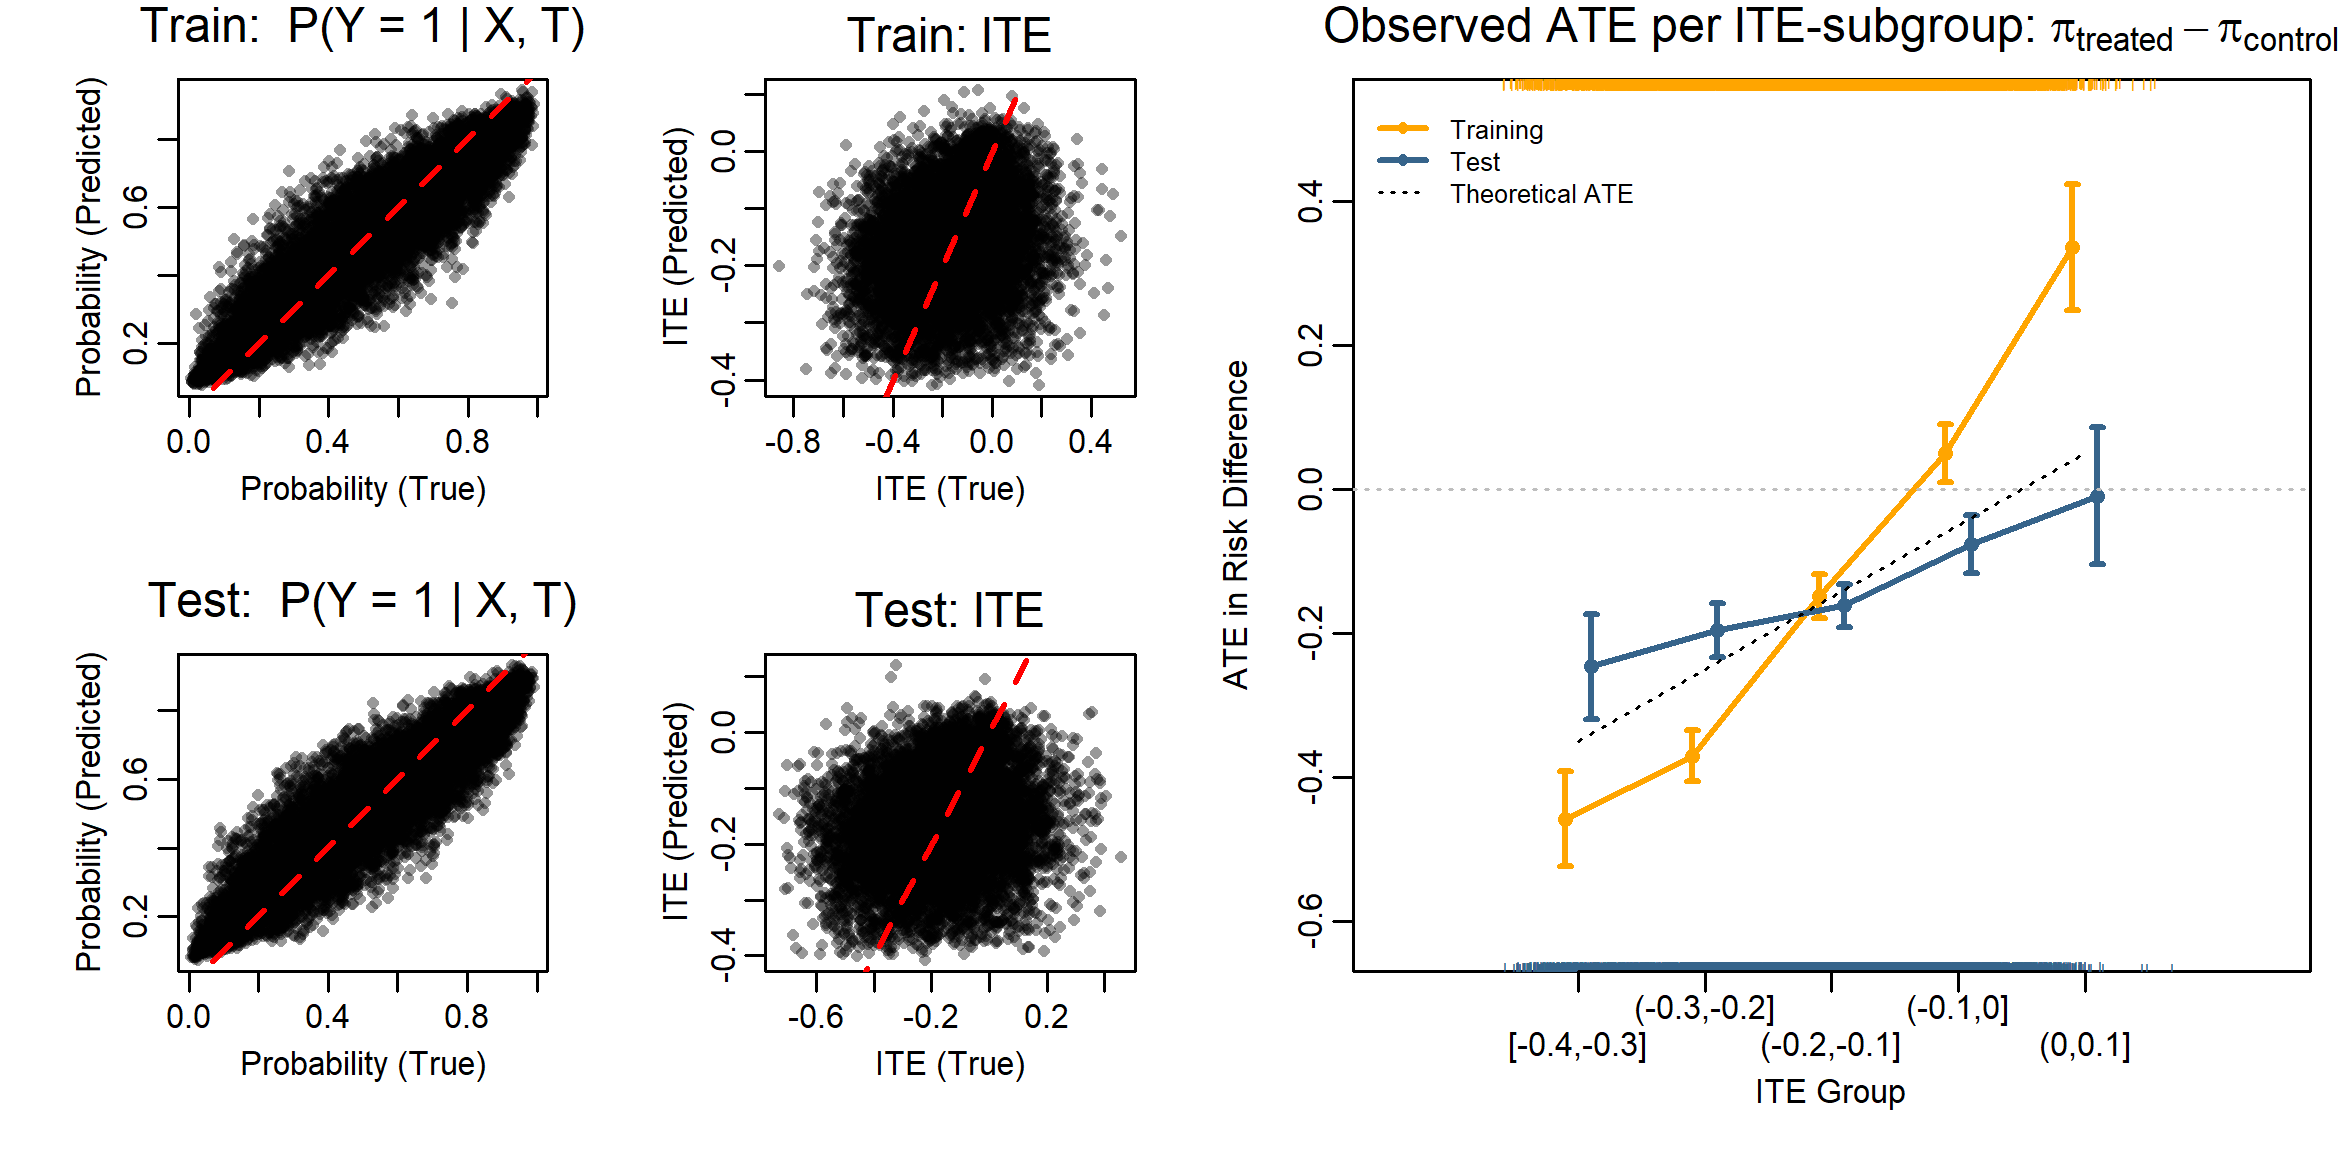
\includegraphics[width=0.9\textwidth]{img/results_ITE_simulation/unobserved_interaction_tuned_rf_tlearner.png}
\caption{Results of the T-learner tuned random forest in Scenario~(2), where there are strong treatment and interaction effects, but variable $X_1$ is not observed. Left: true vs. predicted probabilities for $\text{P}(Y = 1 \mid X, T)$; Middle: true vs. predicted ITEs; Right: observed ATE in terms of risk difference per estimated ITE subgroup.}
\label{fig:unobserved_interaction_tuned_rf_tlearner}
\end{figure}


\clearpage

\subsection{Scenario (3): Fully observed, small effects}

\begin{figure}[htbp]
\centering
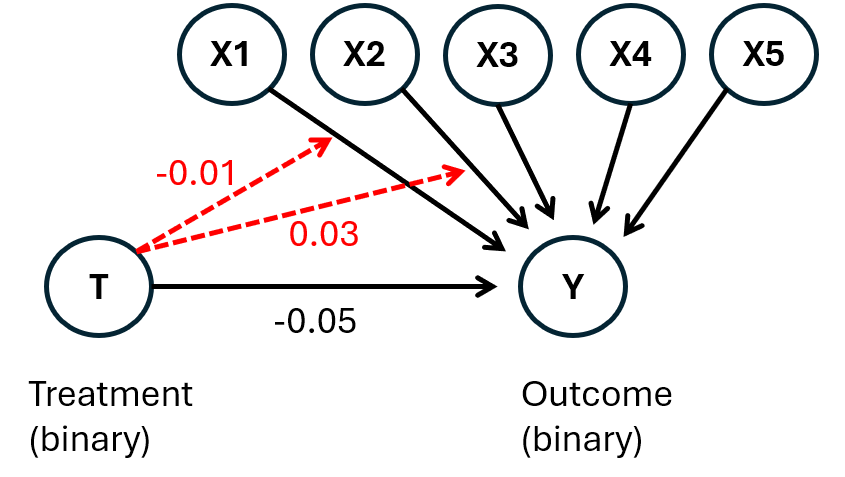
\includegraphics[width=0.35\textwidth]{img/results_ITE_simulation/simulation_small_effects.png}
\caption{DAG for Scenario~(3), where all variables are observed and both treatment and interaction effects are weak. The numbers indicate the coefficients on the log-odds scale. Red arrows represent interaction effects between treatment ($T$) and covariates ($X_1$ and $X_2$) on the outcome ($Y$).}
\label{fig:small_interaction_dag}
\end{figure}




\begin{figure}[htbp]
\centering
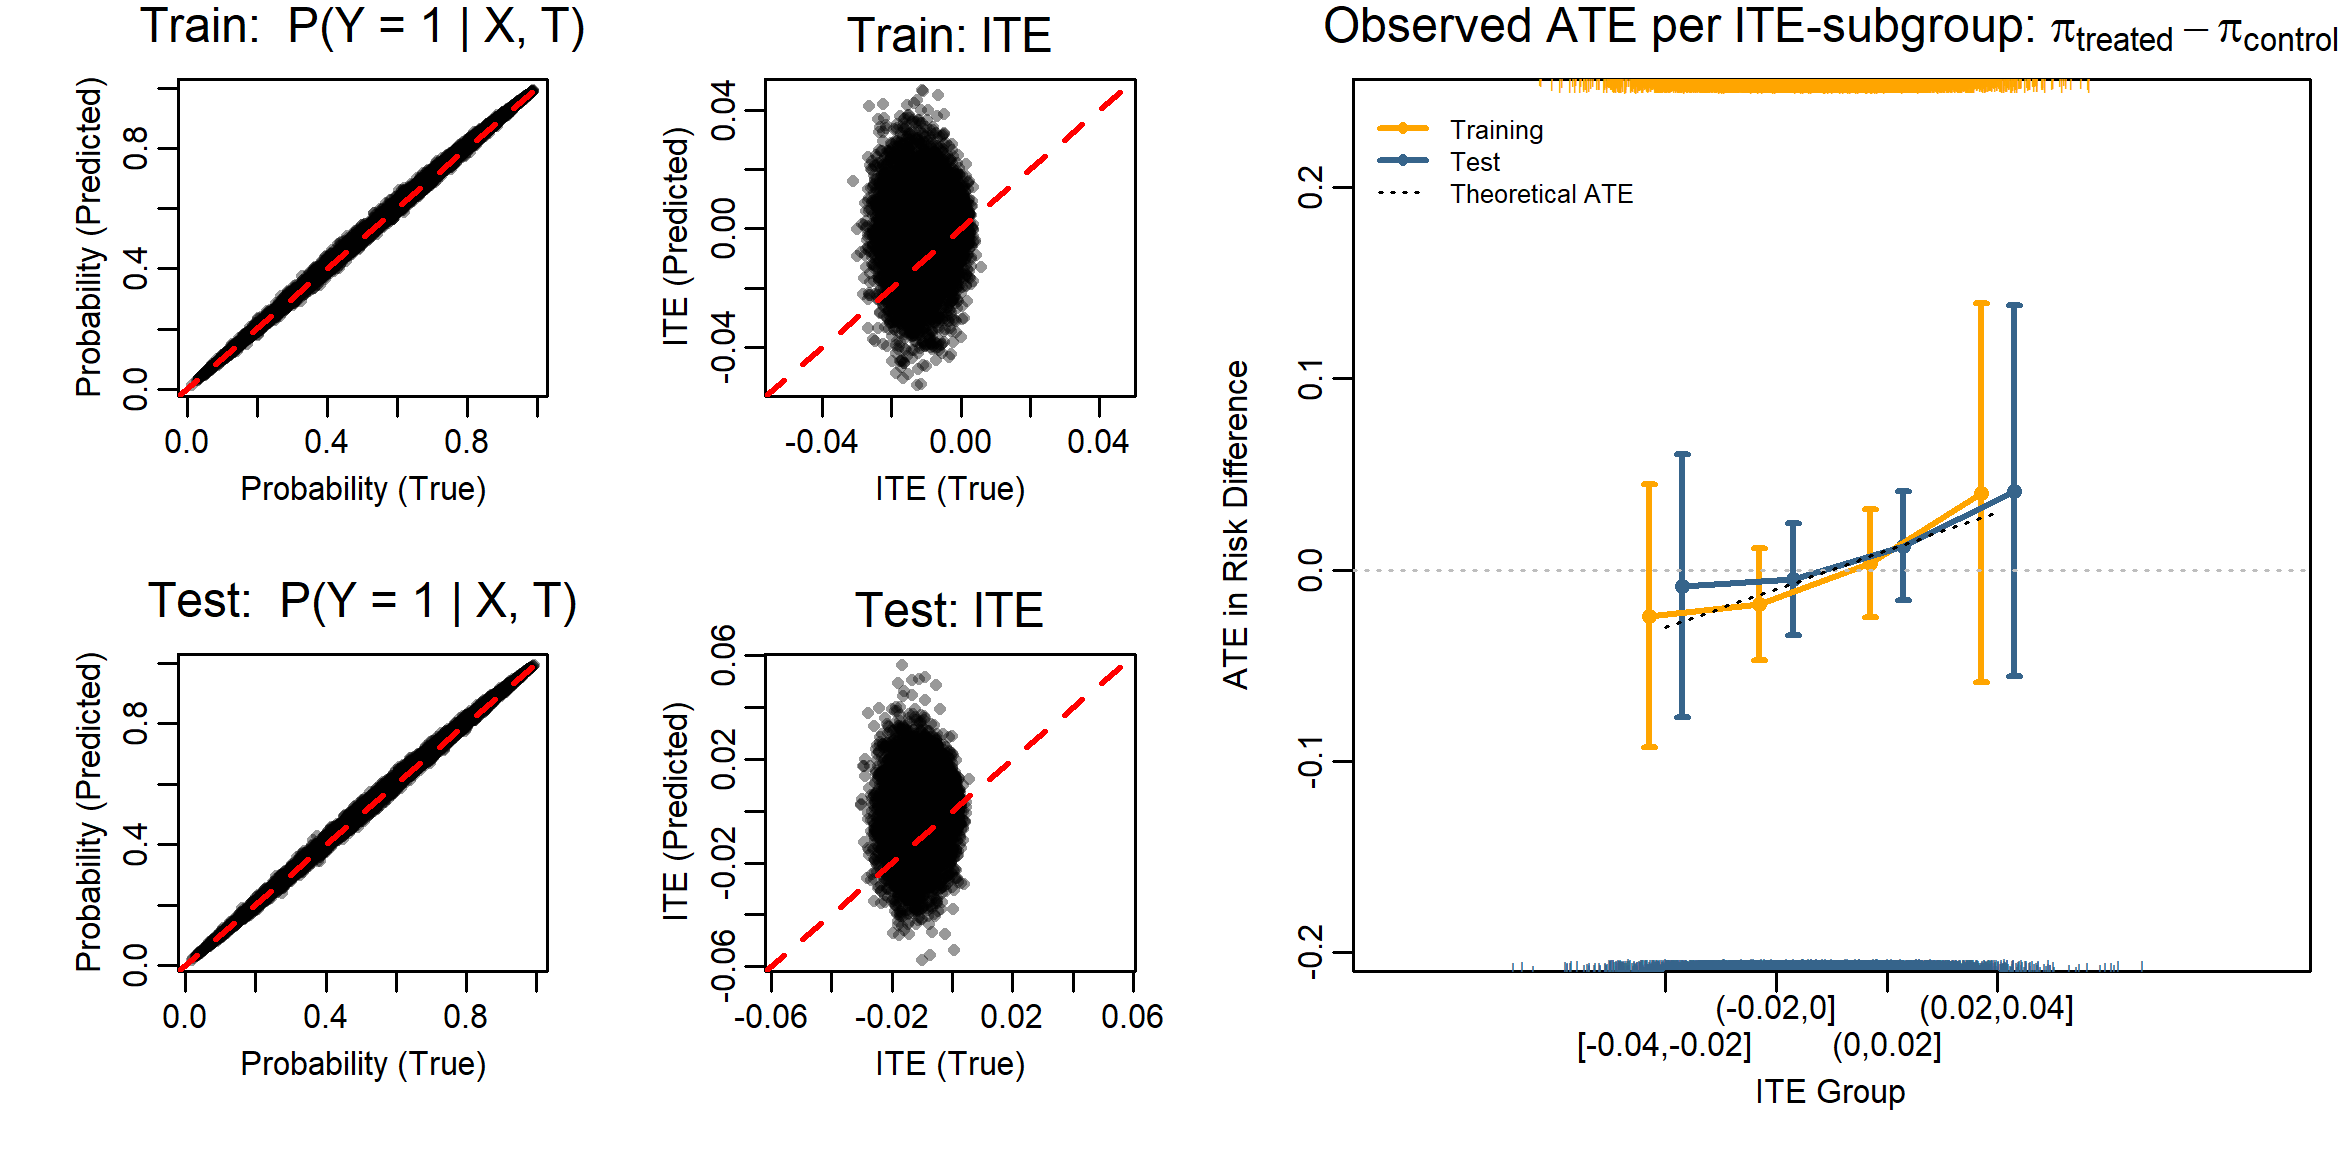
\includegraphics[width=0.9\textwidth]{img/results_ITE_simulation/small_interaction_glm_tlearner.png}
\caption{Results of the T-learner logistic regression in Scenario~(3), where the DAG is fully observed and both treatment and interaction effects are weak. Left: true vs. predicted probabilities for $\text{P}(Y = 1 \mid X, T)$; Middle: true vs. predicted ITEs; Right: observed ATE in terms of risk difference per estimated ITE subgroup.}
\label{fig:small_interaction_glm_tlearner}
\end{figure}




\begin{figure}[htbp]
\centering
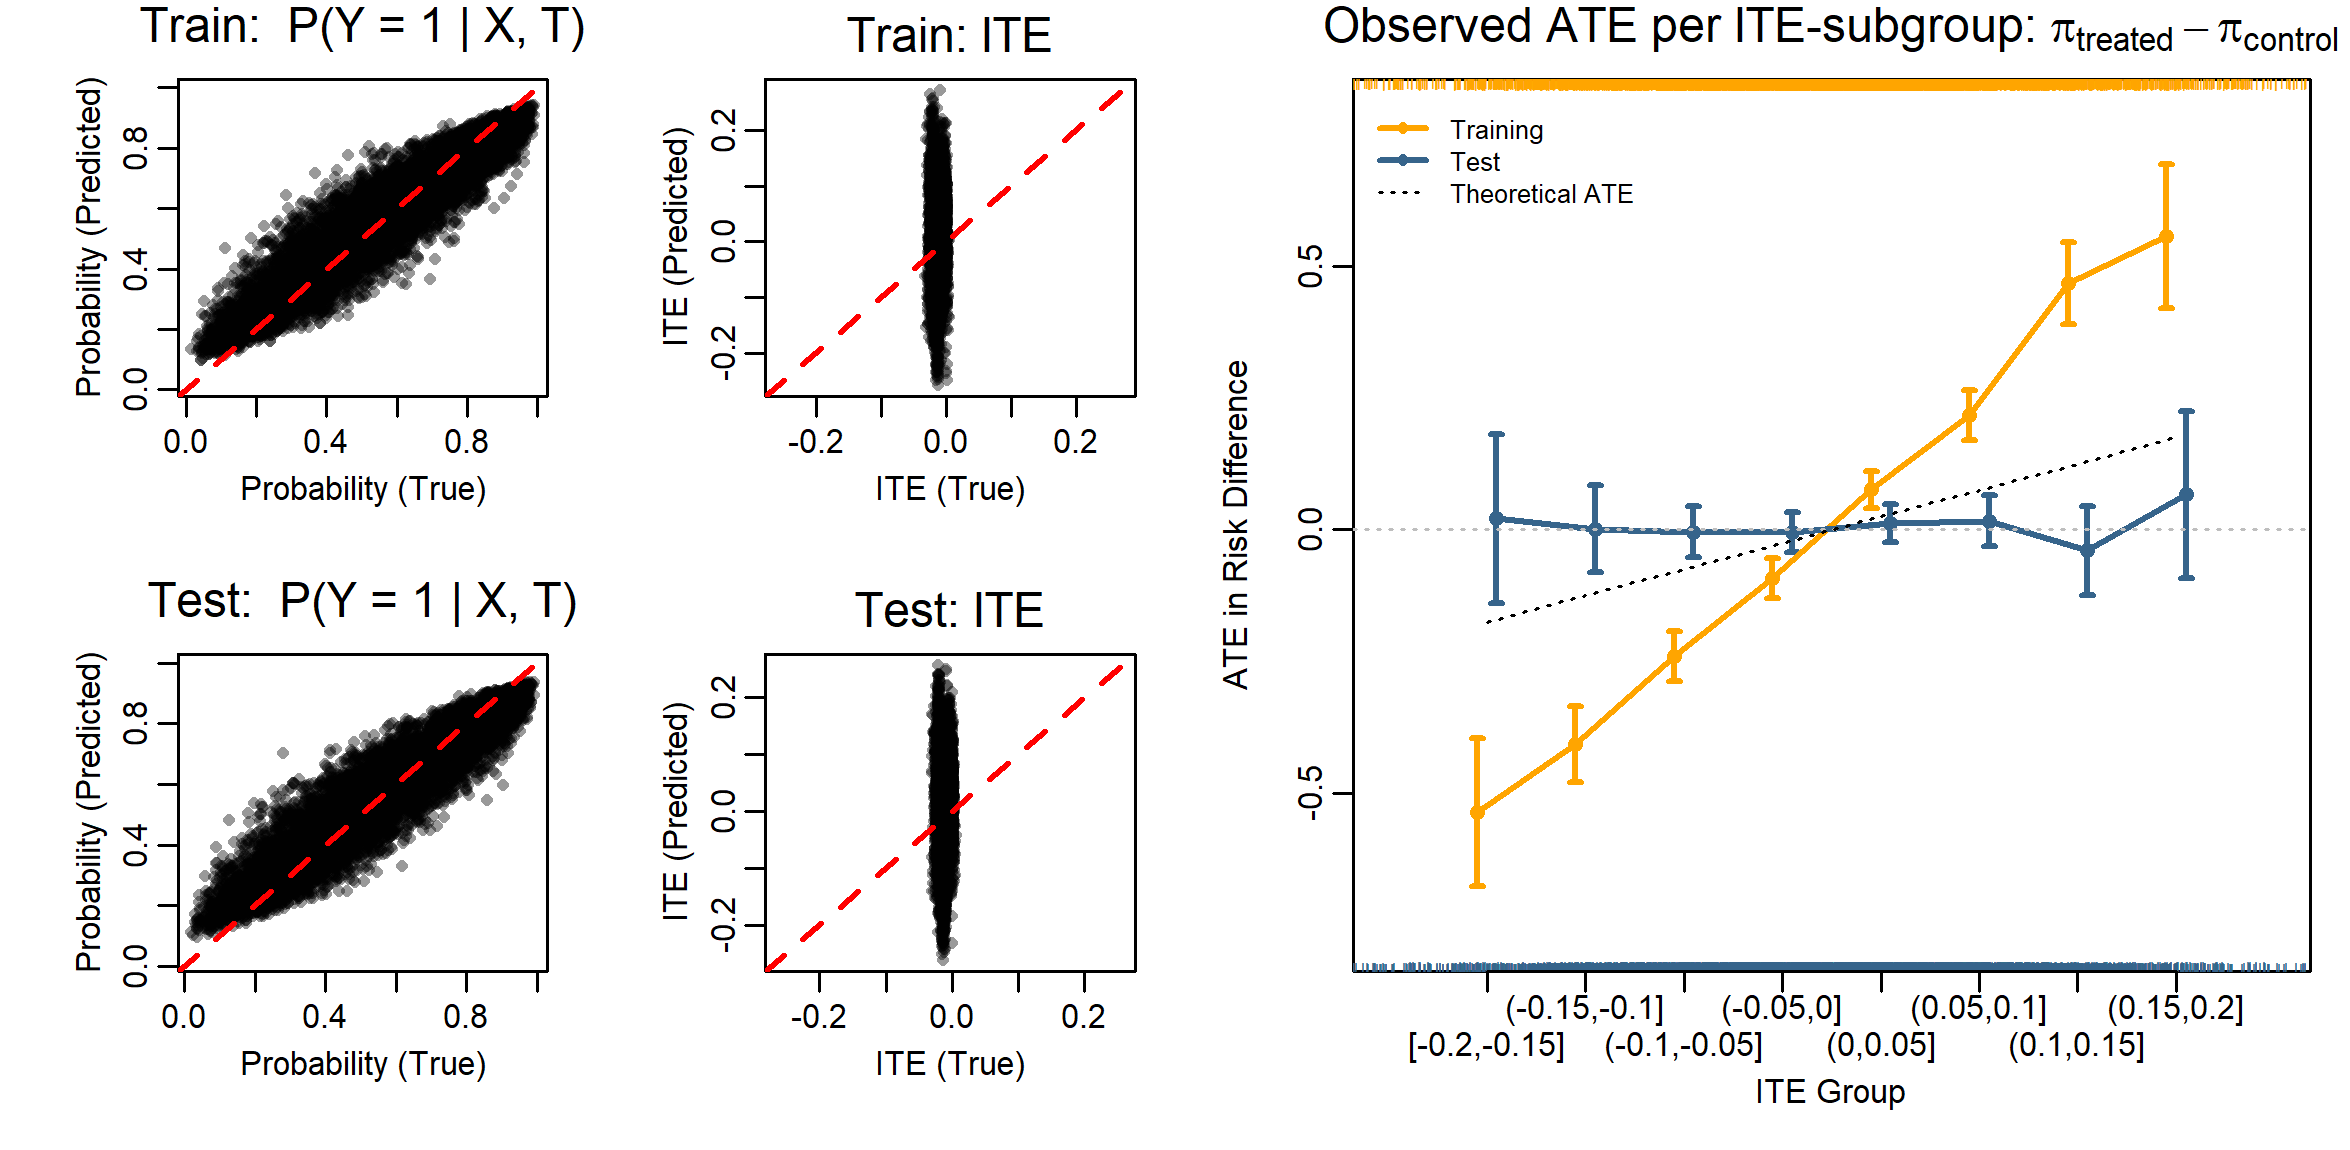
\includegraphics[width=0.9\textwidth]{img/results_ITE_simulation/small_interaction_tuned_rf_tlearner.png}
\caption{Results of the T-learner tuned random forest in Scenario~(3), where the DAG is fully observed and both treatment and interaction effects are weak. Left: true vs. predicted probabilities for $\text{P}(Y = 1 \mid X, T)$; Middle: true vs. predicted ITEs; Right: observed ATE in terms of risk difference per estimated ITE subgroup.}
\label{fig:small_interaction_tuned_rf_tlearner}
\end{figure}


\clearpage


\section{Experiment 4: ITE estimation with TRAM-DAGs (simulation)}

First, we present the results for Scenario (1), which includes both direct and interaction effects  of treatment. Then, we show the results for Scenario (2), which has a direct effect but no interaction effects, and finally Scenario (3), which includes interaction effects but no direct treatment effect. For each scenario, we compare the results in an observational setting with confounded treatment allocation and in a randomized controlled trial (RCT) setting without confounding. We also compare the average treatment effect (ATE), which can be directly calculated in the RCT setting on observed outcomes, with the ATE derived from the estimated ITEs. All ITEs presented in this section are technically quantile treatment effects (QTEs) based on the 0.5-quantile of the potential outcomes. For simplicity, we will refer to them as ITEs. The aim is to investigate how the TRAM-DAG performs in the presence or absence of direct and interaction effects of the treatment, both in confounded and in randomized settings, for the purpose of ITE estimation.

\subsection{Scenario (1): Direct and interaction effects} 


\begin{figure}[H]
\centering
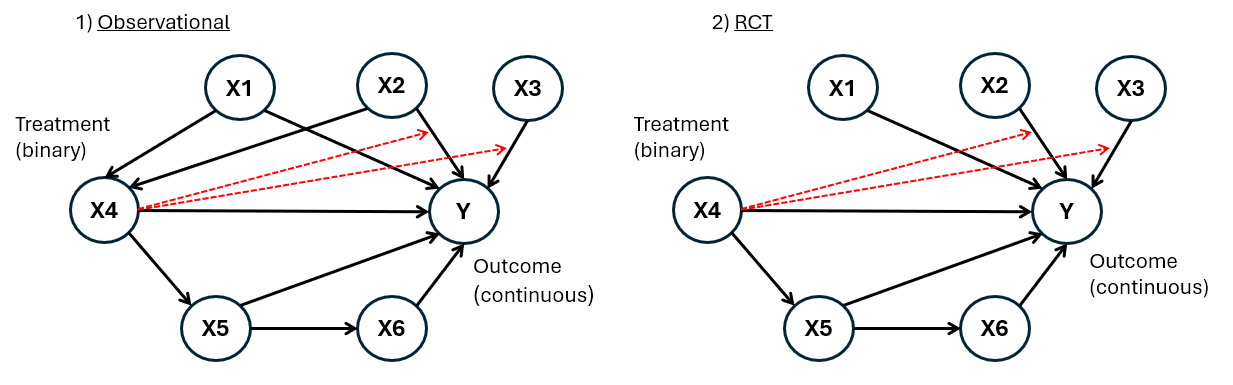
\includegraphics[width=0.85\textwidth]{img/exp4_dags.png}
\caption{DAGs for Scenario~(1), which includes a direct effect of the treatment on the outcome and additional interaction effects with covariates $X_2$ and $X_3$. Left: observational setting; Right: RCT setting.}
\label{fig:ite_dag_observational_1}
\end{figure}

Scenario~(1) includes a direct effect of the treatment on the outcome, and interaction effects with $X_2$ and $X_3$, as shown in Figure~\ref{fig:ite_dag_observational_1}. Train and test sets with 20,000 samples each were generated.

In the observational setting, treatment was confounded by $X_1$ and $X_2$. In the train set, $38.6$\% of individuals were in the control group and $61.4$\% in the treatment group. The test set had a similar distribution.

In the RCT setting, treatment was randomly assigned. In the train set, $49.8$\% were in control and $50.2$\% in treatment; in the test set, the shares were $50.2$\% and $49.8$\%, respectively.

Figure~\ref{fig:scenario1_ite_distribution_dgp} shows the true ITE distribution from the DGP, which displays some heterogeneity due to interaction effects. Figure~\ref{fig:scenario1_sampling_distributions_vertical} shows the marginal distributions of all variables in the DGP and as estimated by the TRAM-DAG. The distribution of the outcome $Y$ under $\text{do}(X_4 = 0)$ and $\text{do}(X_4 = 1)$ is shown in Figure~\ref{fig:scenario1_outcome_distributions}. The ITEs were estimated as the difference in medians of the potential outcomes. Figure~\ref{fig:scenario1_ite_densities_train_test} compares the densities of the estimated and true ITEs. In both observational and RCT settings, the estimated ITEs are close to the true ones in both train and test sets. Figure~\ref{fig:scenario1_ite_scatter_train_test} shows the scatterplots of estimated vs. true ITEs. Figures~\ref{fig:observ_scenario1_ite_ATE} and \ref{fig:rct_scenario1_ite_ATE} show the ITE-ATE plots, where the ATE is calculated as the median difference in observed outcomes within ITE subgroups. The trends are similar across train and test sets.



The ATEs calculated based on different measures in both the training and test sets are shown in Table~\ref{tab:scenario1_ate_comparison}. In the RCT setting (training set), the difference in means of the outcomes between the two treatment groups was 
$-0.563$, with a confidence interval of 
$-0.582$ to 
$-0.543$. 



% 
% Scenario (1) included a direct effect of the treatment on the outcome and an additional interaction effect of the treatment with the covariates X2 and X3, as presented in Figure~\ref{fig:ite_dag_observational_1}. A train and test set were generated with 20,000 observations each. 
% In the observational setting, the treatment allocation was confounded by the covariates X1 and X2.  In the train set, $round(observ_scenario1$dev_treatment_allocation[1]*100, 1)$\% of patients were in the control group and $round(observ_scenario1$dev_treatment_allocation[2]*100, 1)$\% were in the treatment group. This ratio was similar in the test set. 
% In the RCT setting treatment allocation was randomized. In the train set $round(rct_scenario1$dev_treatment_allocation[1]*100, 1)$\% individuals were in the control group and $round(rct_scenario1$dev_treatment_allocation[2]*100, 1)$\% in the treatment group. In the test set $round(rct_scenario1$val_treatment_allocation[1]*100, 1)$\% were in the control group and $round(rct_scenario1$val_treatment_allocation[2]*100, 1)$\% in the treatment group. 
% Figure \ref{fig:scenario1_ite_distribution_dgp} illustrates the true ITE distribution that resulted from the DGP. Due to the interaction effects, there is some heterogeneity in the ITE distribution. Figure \ref{fig:scenario1_sampling_distributions_vertical} shows the marginal distributions of all variables according to the DGP and the estimates by the fitted TRAM-DAG. Figure \ref{fig:scenario1_outcome_distributions} shows the distribution of the outcome ($Y$) under the do(Tr=0) and do(Tr=1) interventions. The fitted model was applied to estimate the ITEs in terms of the difference in medians of the potential outcomes. The resulting density of the estimated ITEs compared to the true ITEs according to the DGP is shown in Figure \ref{fig:scenario1_ite_densities_train_test}. Across both settings, the densities of the estimated ITEs are close to the true densities in both the training and test datasets. Figure \ref{fig:scenario1_ite_scatter_train_test} shows the scatterplots of true against estimated ITEs. Finally, Figure \ref{fig:scenario1_ite_cATE} displays the ITE-ATE plot where the ATE is computed as the difference in medians of the observed outcome under the treatments within the respective ITE-subgroups. The trends observed in the training and test sets are consistent.


% The average treatment effect (ATE) is presented in Table \ref{tab:scenario1_ate_comparison}. In the RCT setting in the training set, the difference in means of the outcomes in the two treatment groups was $round(rct_scenario1$dev_ATE_observed_Y_mean_diff, 3)$ with a confidence interval of $round(rct_scenario1$dev_ATE_observed_Y_mean_diff_CI[1], 3)$ to $round(rct_scenario1$dev_ATE_observed_Y_mean_diff_CI[2], 3)$. The ATEs calculated based on different measuress in the training and test dataset, are shown in Table \ref{tab:scenario1_ate_comparison}.


% The ATE in terms of the difference in medians of the observed outcomes was $round(rct_scenario1$dev_ATE_observed_Y_median_diff, 3)$. Also in the training set, the ATE in terms of the mean of the true ITEs was $round(rct_scenario1$dev_ITE_median_average, 3)$ and the ATE in terms of the mean of the estimated ITEs was $round(rct_scenario1$dev_ITE_median_pred_average, 3)$. 


\begin{table}[htbp]
\centering
\small
\caption{Scenario (1), including direct and interaction effects: Comparison of ATE measures across train and test sets for the observational and RCT setting. $\text{Y}_\text{observed}^{(\text{Tr})}$ denotes the observed outcome under the treatment ($\text{Tr}$) actually received. The estimated ATE from $\text{mean}(\text{ITE}_\text{estimated})$ can be directly compared to the true $\text{mean}(\text{ITE}_\text{true})$, whereas comparisons to the empirical ATEs based on outcome differences should be interpreted with caution.}
\label{tab:scenario1_ate_comparison}
\begin{tabular}{l c c c c}
\toprule
\textbf{Measure} & \multicolumn{2}{c}{\textbf{Observational}} & \multicolumn{2}{c}{\textbf{RCT}} \\
\cmidrule(lr){2-3} \cmidrule(lr){4-5}
 & \textbf{Train} & \textbf{Test} & \textbf{Train} & \textbf{Test} \\
\midrule
ATE as $\text{mean}(\text{Y}_\text{observed}^{(1)}) - \text{mean}(\text{Y}_\text{observed}^{(0)})$ 
& NA & NA 
& -0.563 
& -0.563 \\

ATE as $\text{median}(\text{Y}_\text{observed}^{(1)}) - \text{median}(\text{Y}_\text{observed}^{(0)})$  
& NA & NA 
& -0.626 
& -0.638 \\

ATE as mean(ITE$_\text{true}$)  
& -0.620 
& -0.622 
& -0.620 
& -0.622 \\

ATE as mean(ITE$_\text{estimated}$) 
& -0.617 
& -0.620 
& -0.619 
& -0.622 \\
\bottomrule
\end{tabular}
\end{table}

% 
% \begin{table}[htbp]
% \centering
% \small
% \caption{Scenario (1), including direct and interaction effects: Comparison of ATE measures across train and test sets for the observational and RCT setting.}
% \label{tab:scenario1_ate_comparison_old}
% \begin{tabular}{l c c c c}
% \toprule
% \textbf{Measure} & \multicolumn{2}{c}{\textbf{Observational}} & \multicolumn{2}{c}{\textbf{RCT}} \\
% \cmidrule(lr){2-3} \cmidrule(lr){4-5}
%  & \textbf{Train} & \textbf{Test} & \textbf{Train} & \textbf{Test} \\
% \midrule
% ATE as $\text{mean}(\text{Y}_\text{observed}^{(1)}) - \text{mean}(\text{Y}_\text{observed}^{(0)})$ & NA & NA & round(rct_scenario1$dev_ATE_observed_Y_mean_diff, 3) & round(rct_scenario1$val_ATE_observed_Y_mean_diff, 3) \\
% ATE as $\text{median}(\text{Y}_\text{observed}^{(1)}) - \text{median}(\text{Y}_\text{observed}^{(0)})$  & NA & NA & round(rct_scenario1$dev_ATE_observed_Y_median_diff, 3) & round(rct_scenario1$val_ATE_observed_Y_median_diff, 3) \\
% ATE as mean(ITE$_\text{true}$)  & round(observ_scenario1$dev_ITE_median_average, 3) & round(observ_scenario1$val_ITE_median_average, 3) & round(rct_scenario1$dev_ITE_median_average, 3) & round(rct_scenario1$val_ITE_median_average, 3) \\
% ATE as mean(ITE$_\text{estimated}$) & round(observ_scenario1$dev_ITE_median_pred_average, 3) & round(observ_scenario1$val_ITE_median_pred_average, 3) & round(rct_scenario1$dev_ITE_median_pred_average, 3) & round(rct_scenario1$val_ITE_median_pred_average, 3) \\
% \bottomrule
% \end{tabular}
% \end{table}




\begin{figure}[htbp]
\centering
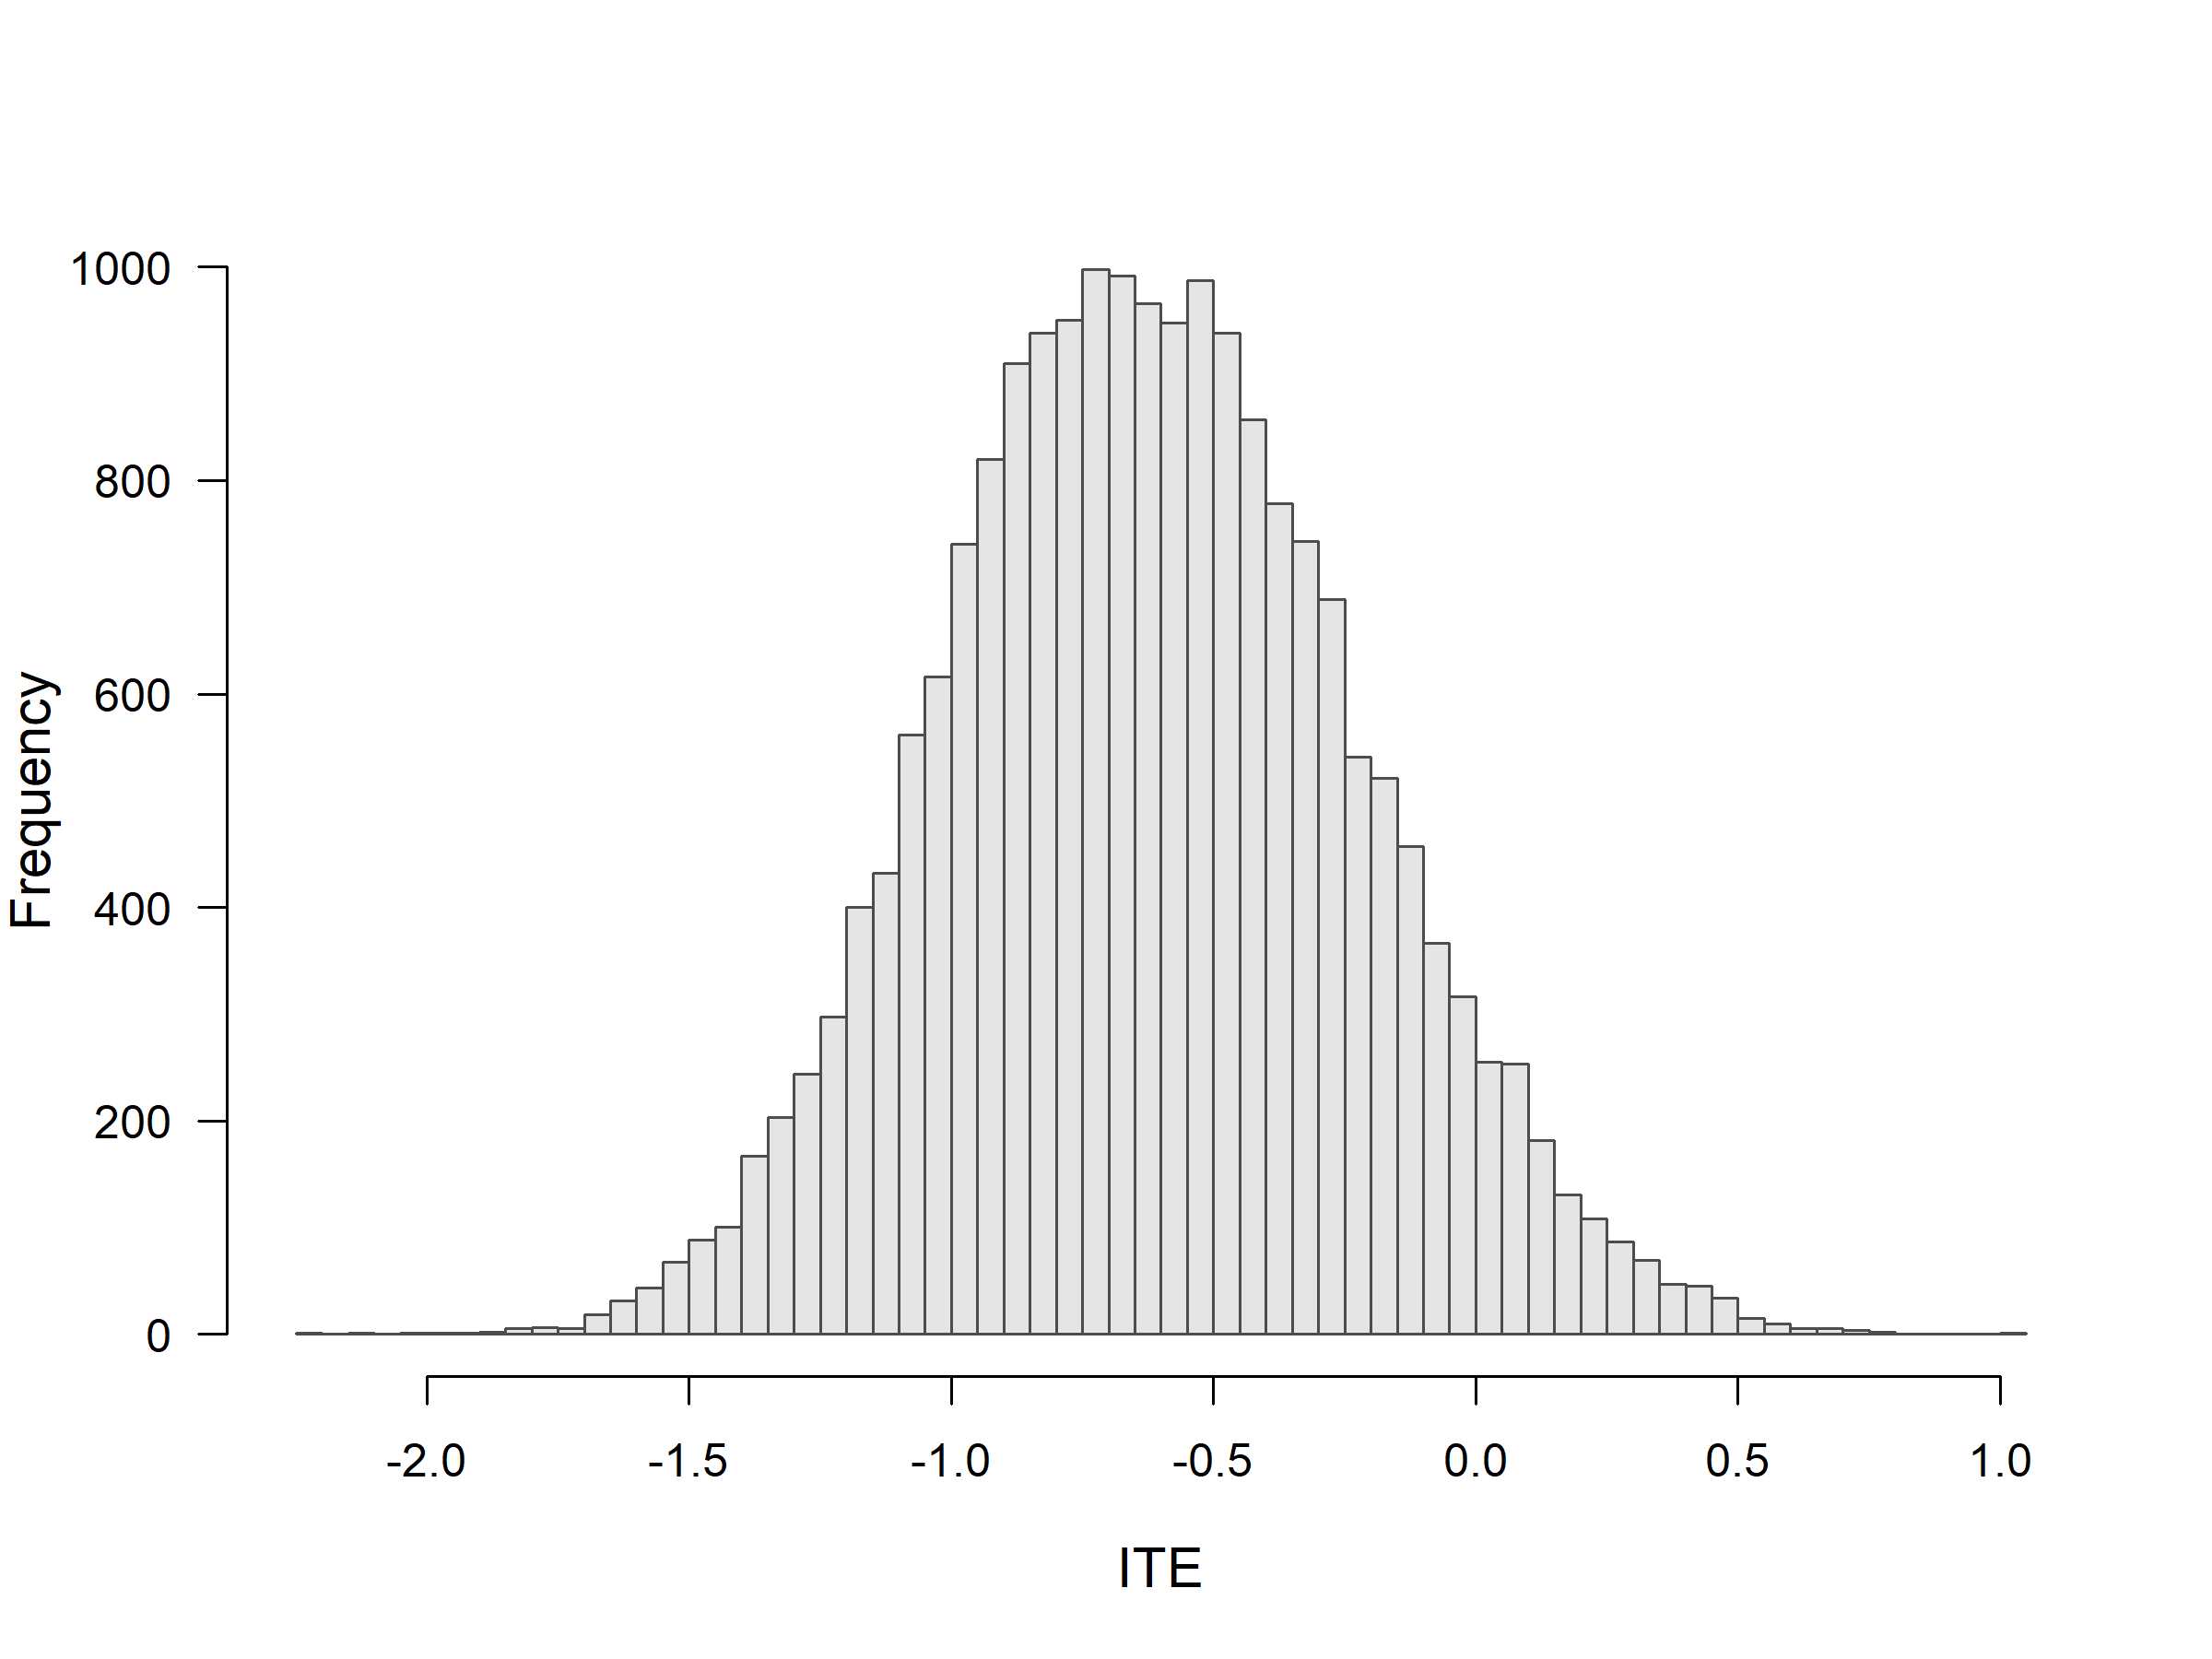
\includegraphics[width=0.7\textwidth]{img/results/observ_scenario1_ite_distribution_dgp.png}
\caption{True ITE distribution resulting from the DGP for Scenario (1), which includes both direct and interaction effects. The true ITEs are identical for each individual in the observational and RCT settings, as they are based on the potential outcomes under both treatment conditions.}
\label{fig:scenario1_ite_distribution_dgp}
\end{figure}



\begin{figure}[htbp]
\centering
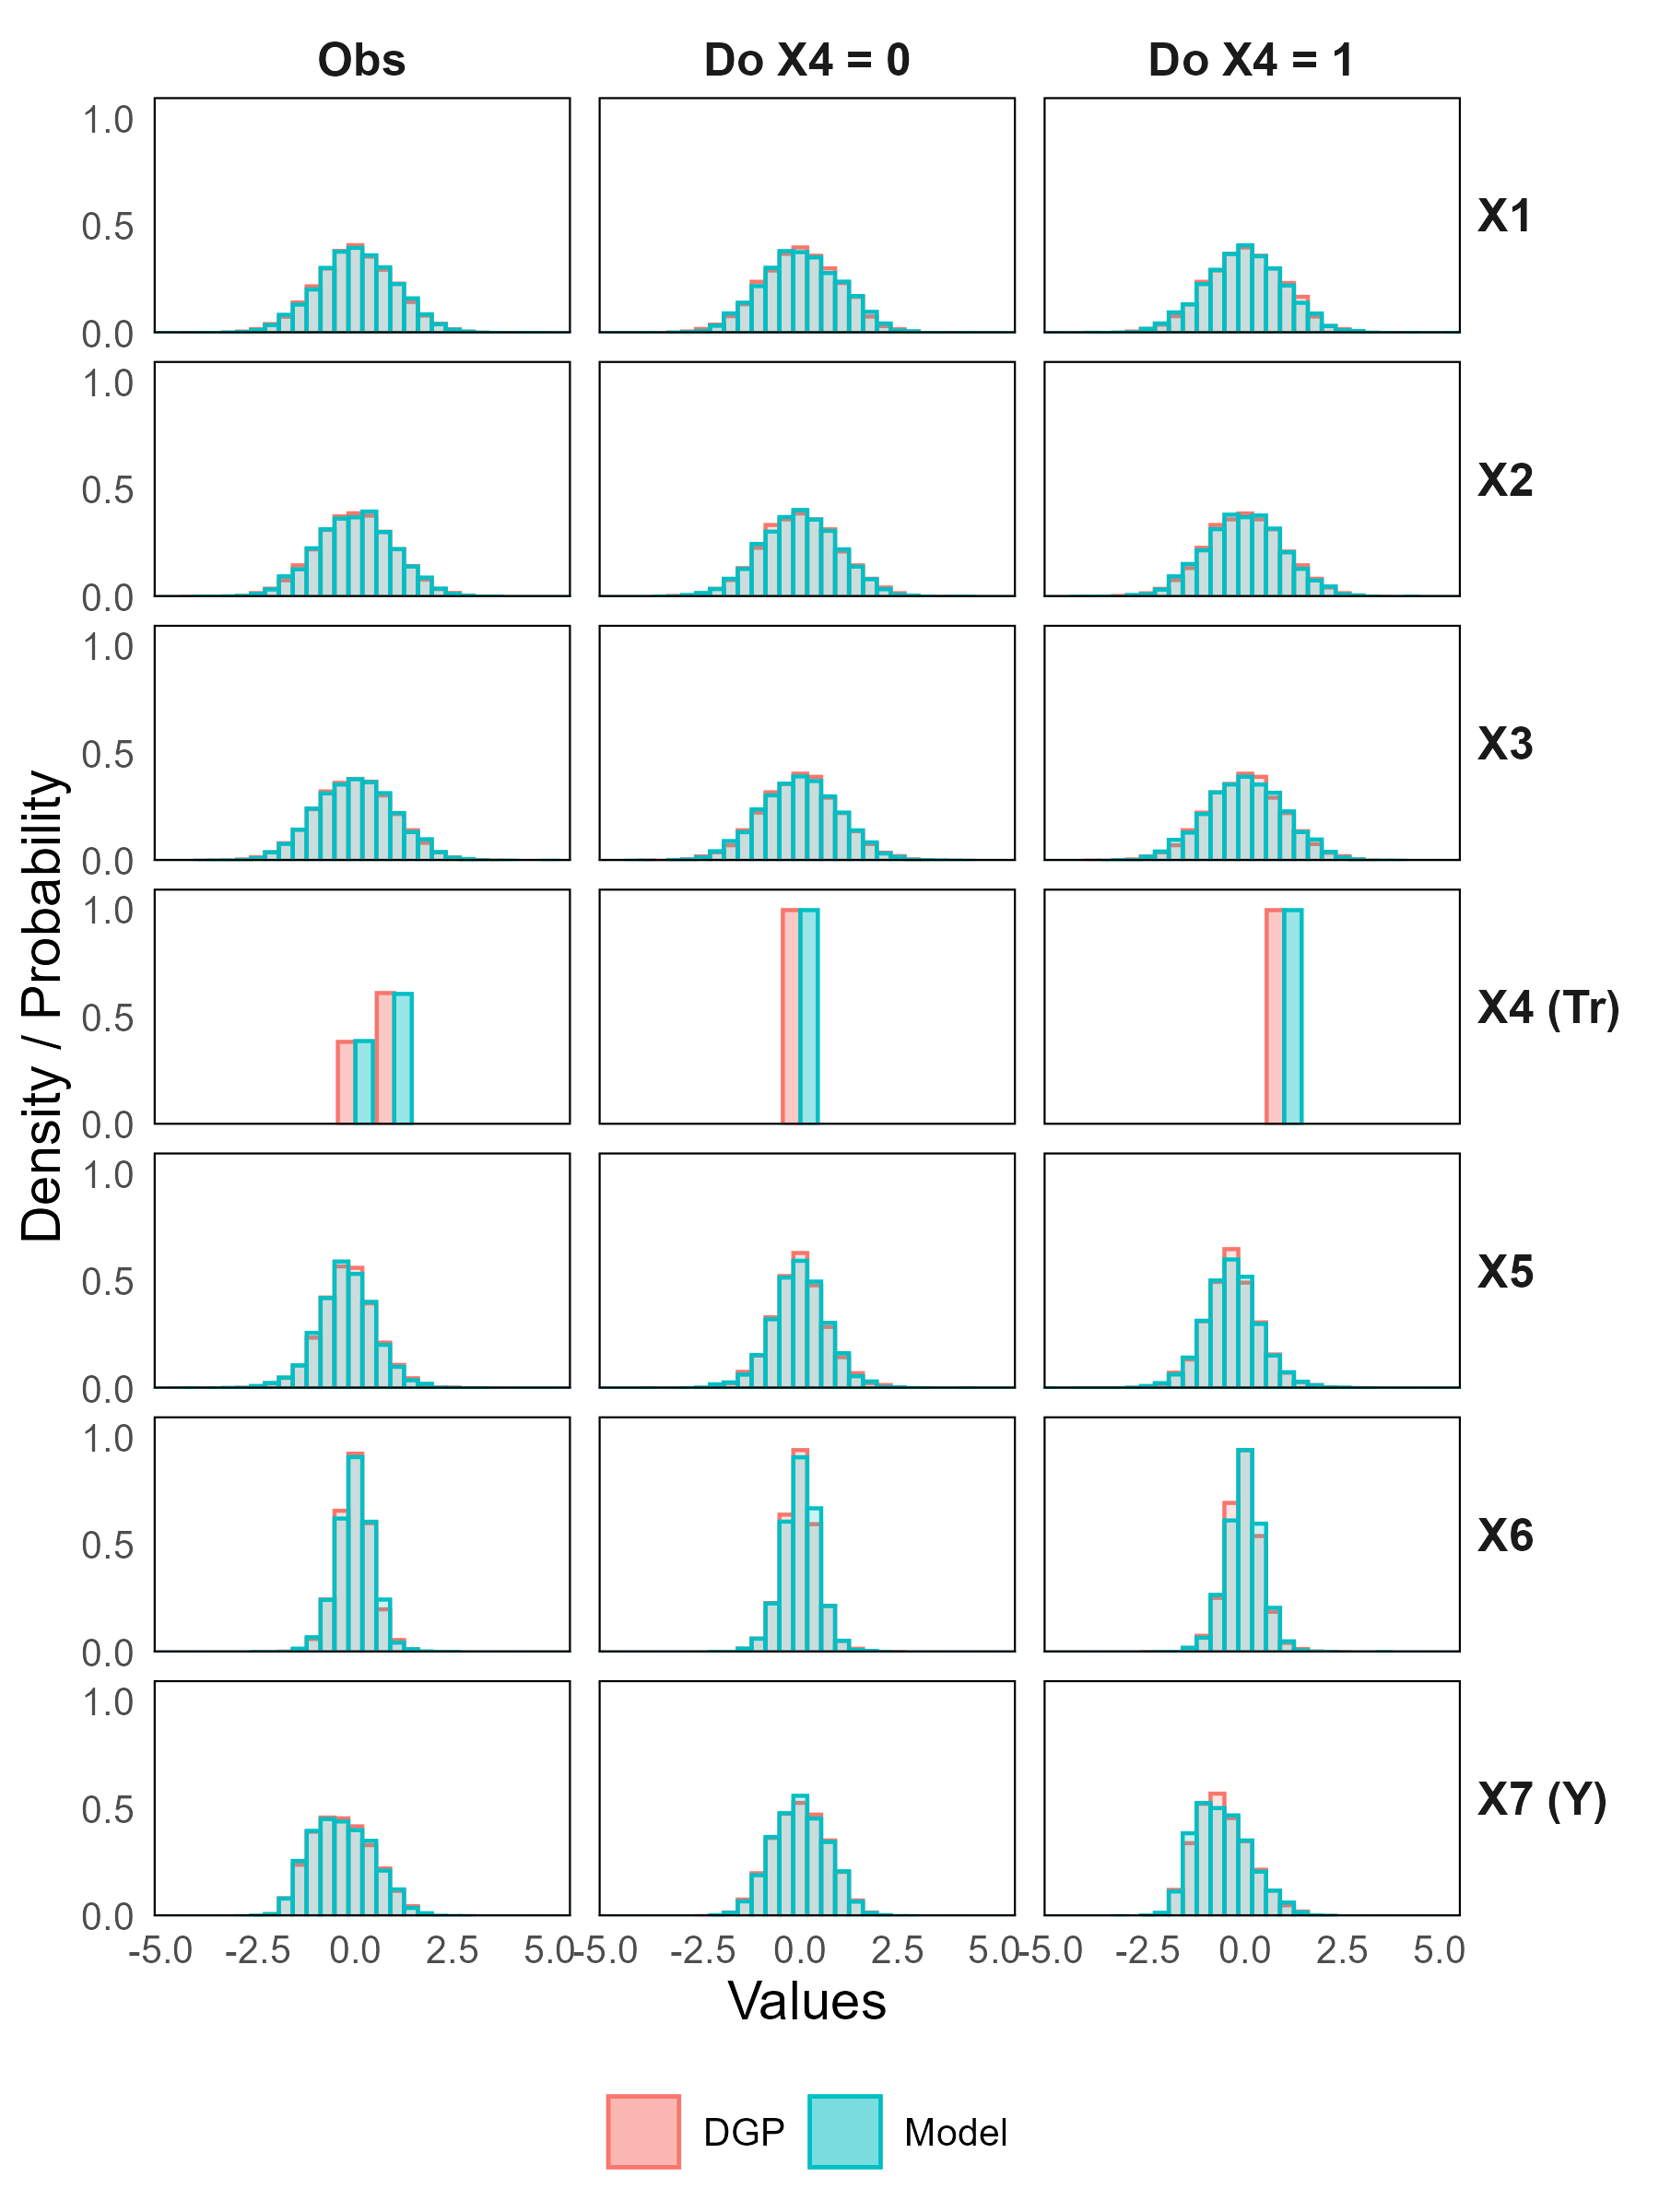
\includegraphics[width=0.45\textwidth]{img/results/observ_scenario1_sampling_distributions_vertical.png}
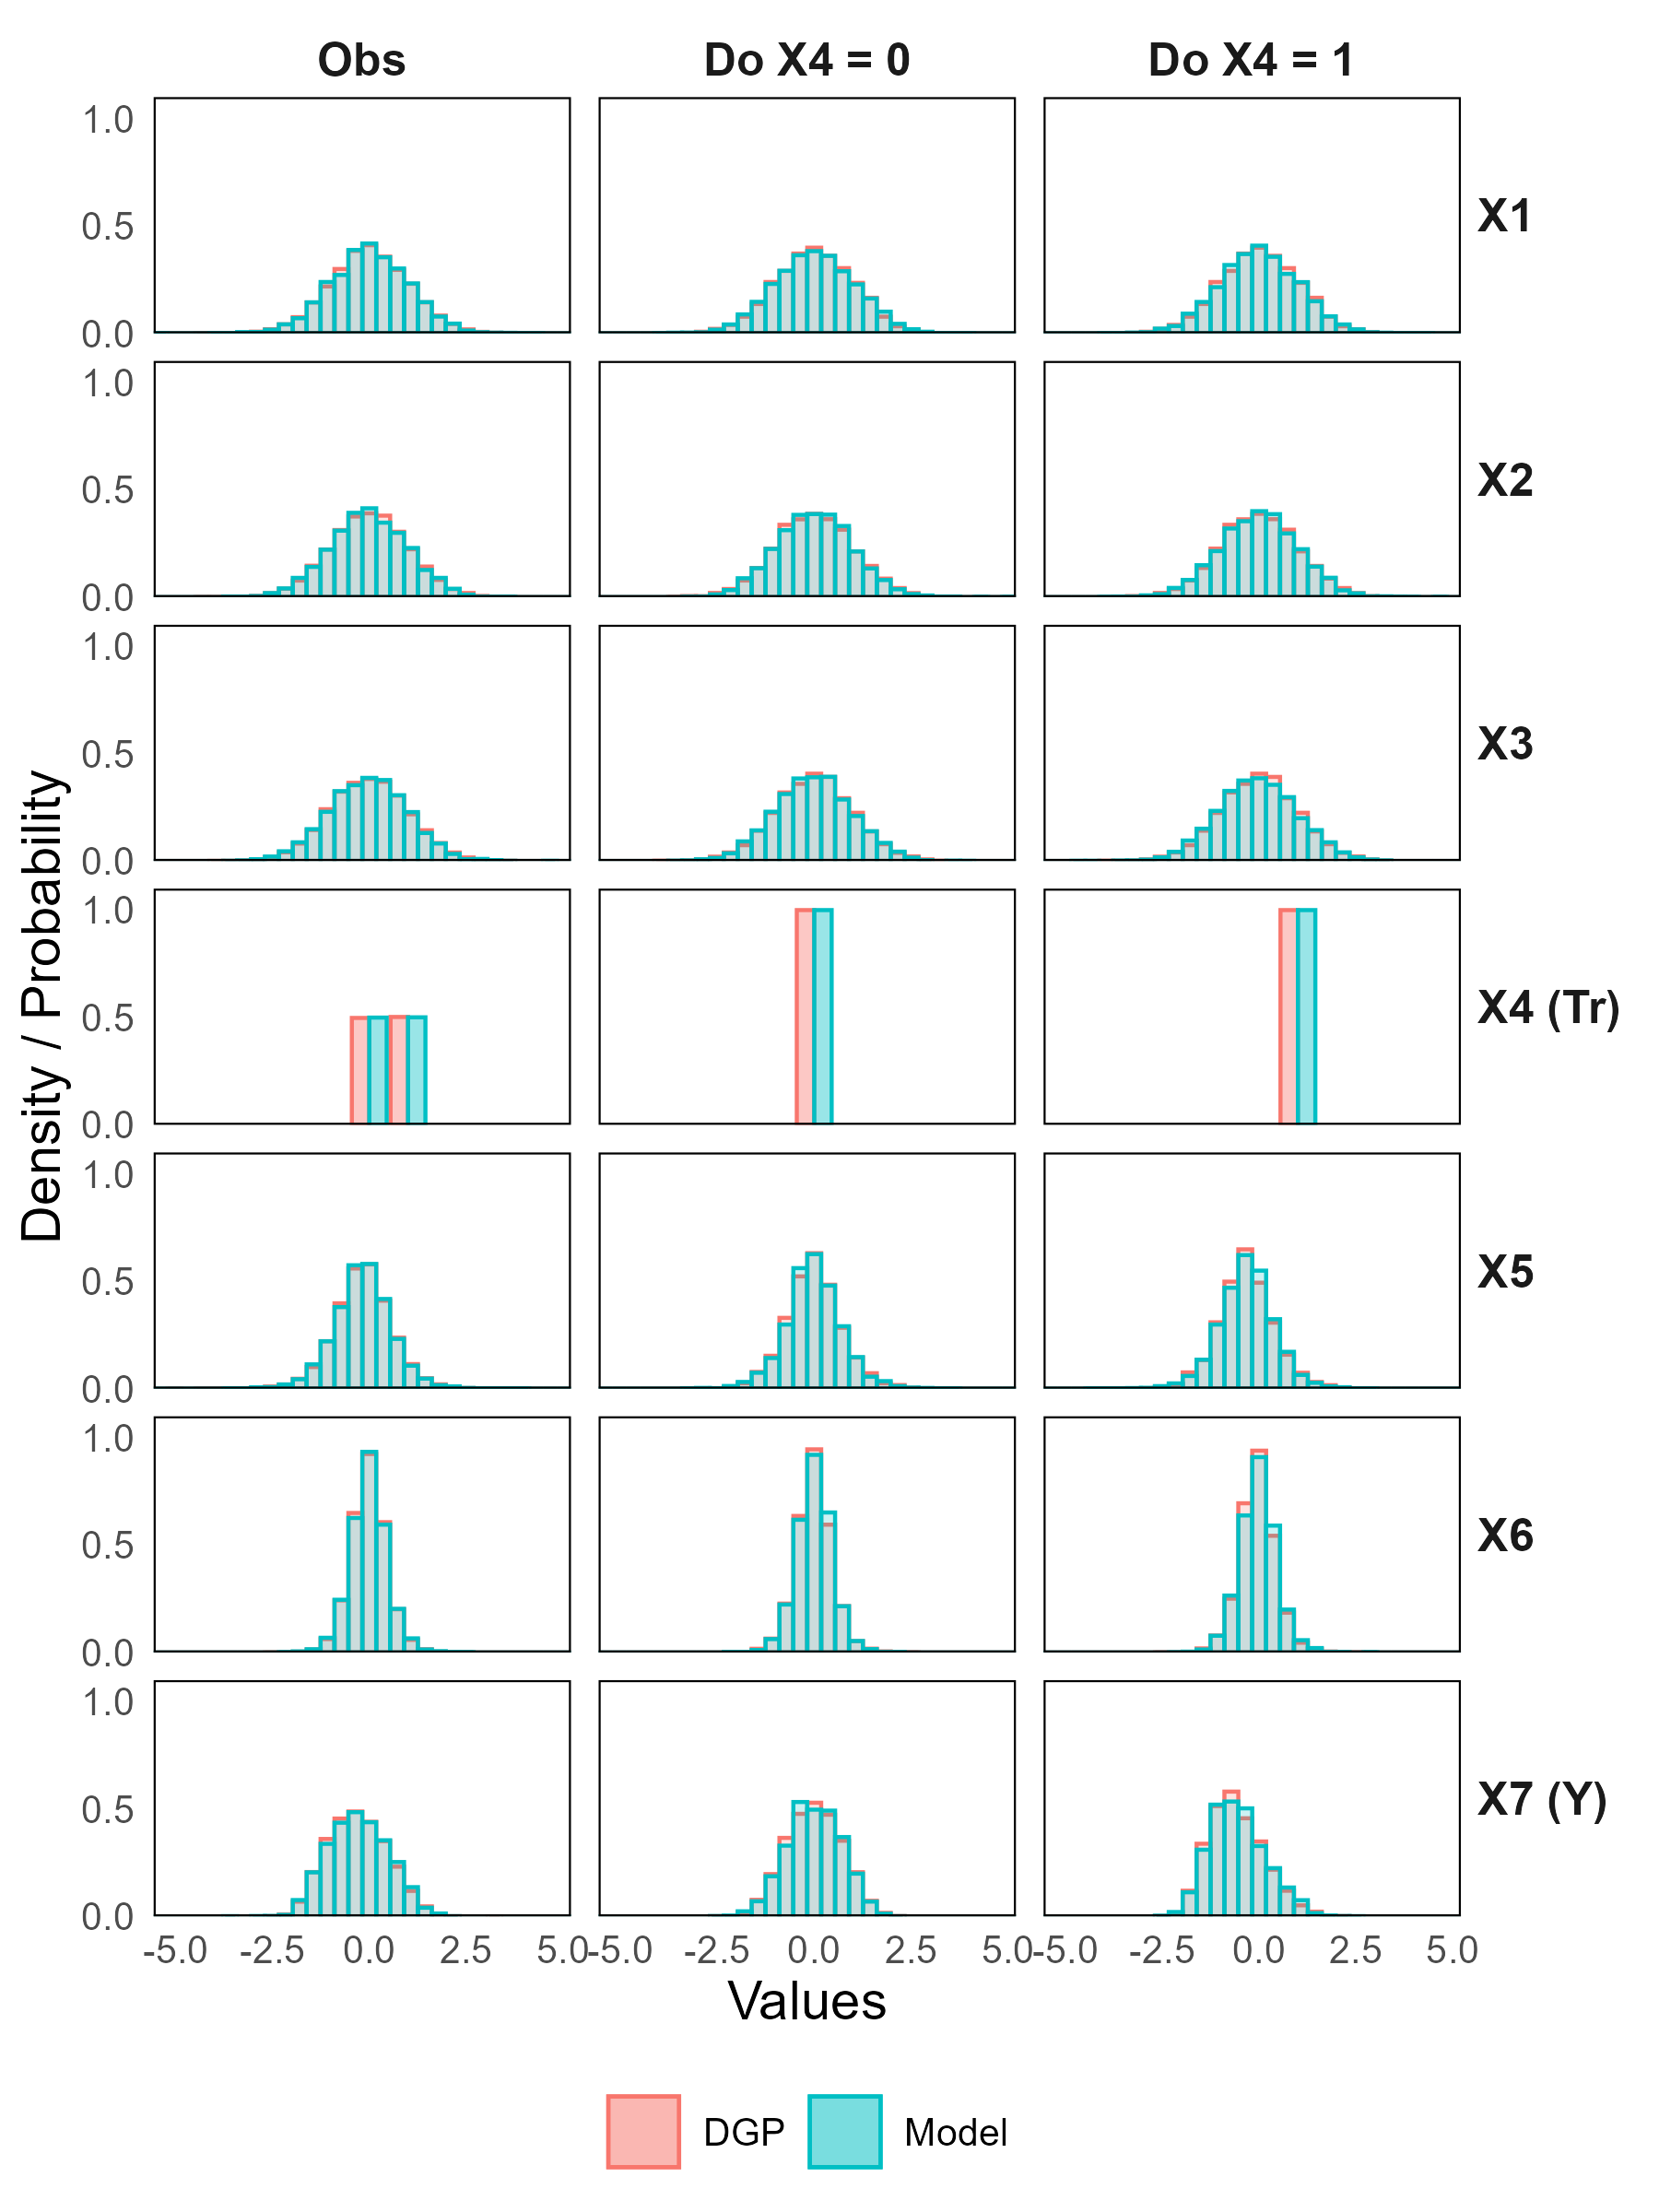
\includegraphics[width=0.45\textwidth]{img/results/rct_scenario1_sampling_distributions_vertical.png}
\caption{Marginal distributions of variables from the DGP and from samples generated by the fitted TRAM-DAG for Scenario (1) with direct and interaction effects. Distributions are shown as observed (Obs), under the control intervention (do($X_4 = 0$)), and under the treatment intervention (do($X_4 = 1$)). Left: Observational; Right: RCT setting.}
\label{fig:scenario1_sampling_distributions_vertical}
\end{figure}


\begin{figure}[htbp]
\centering
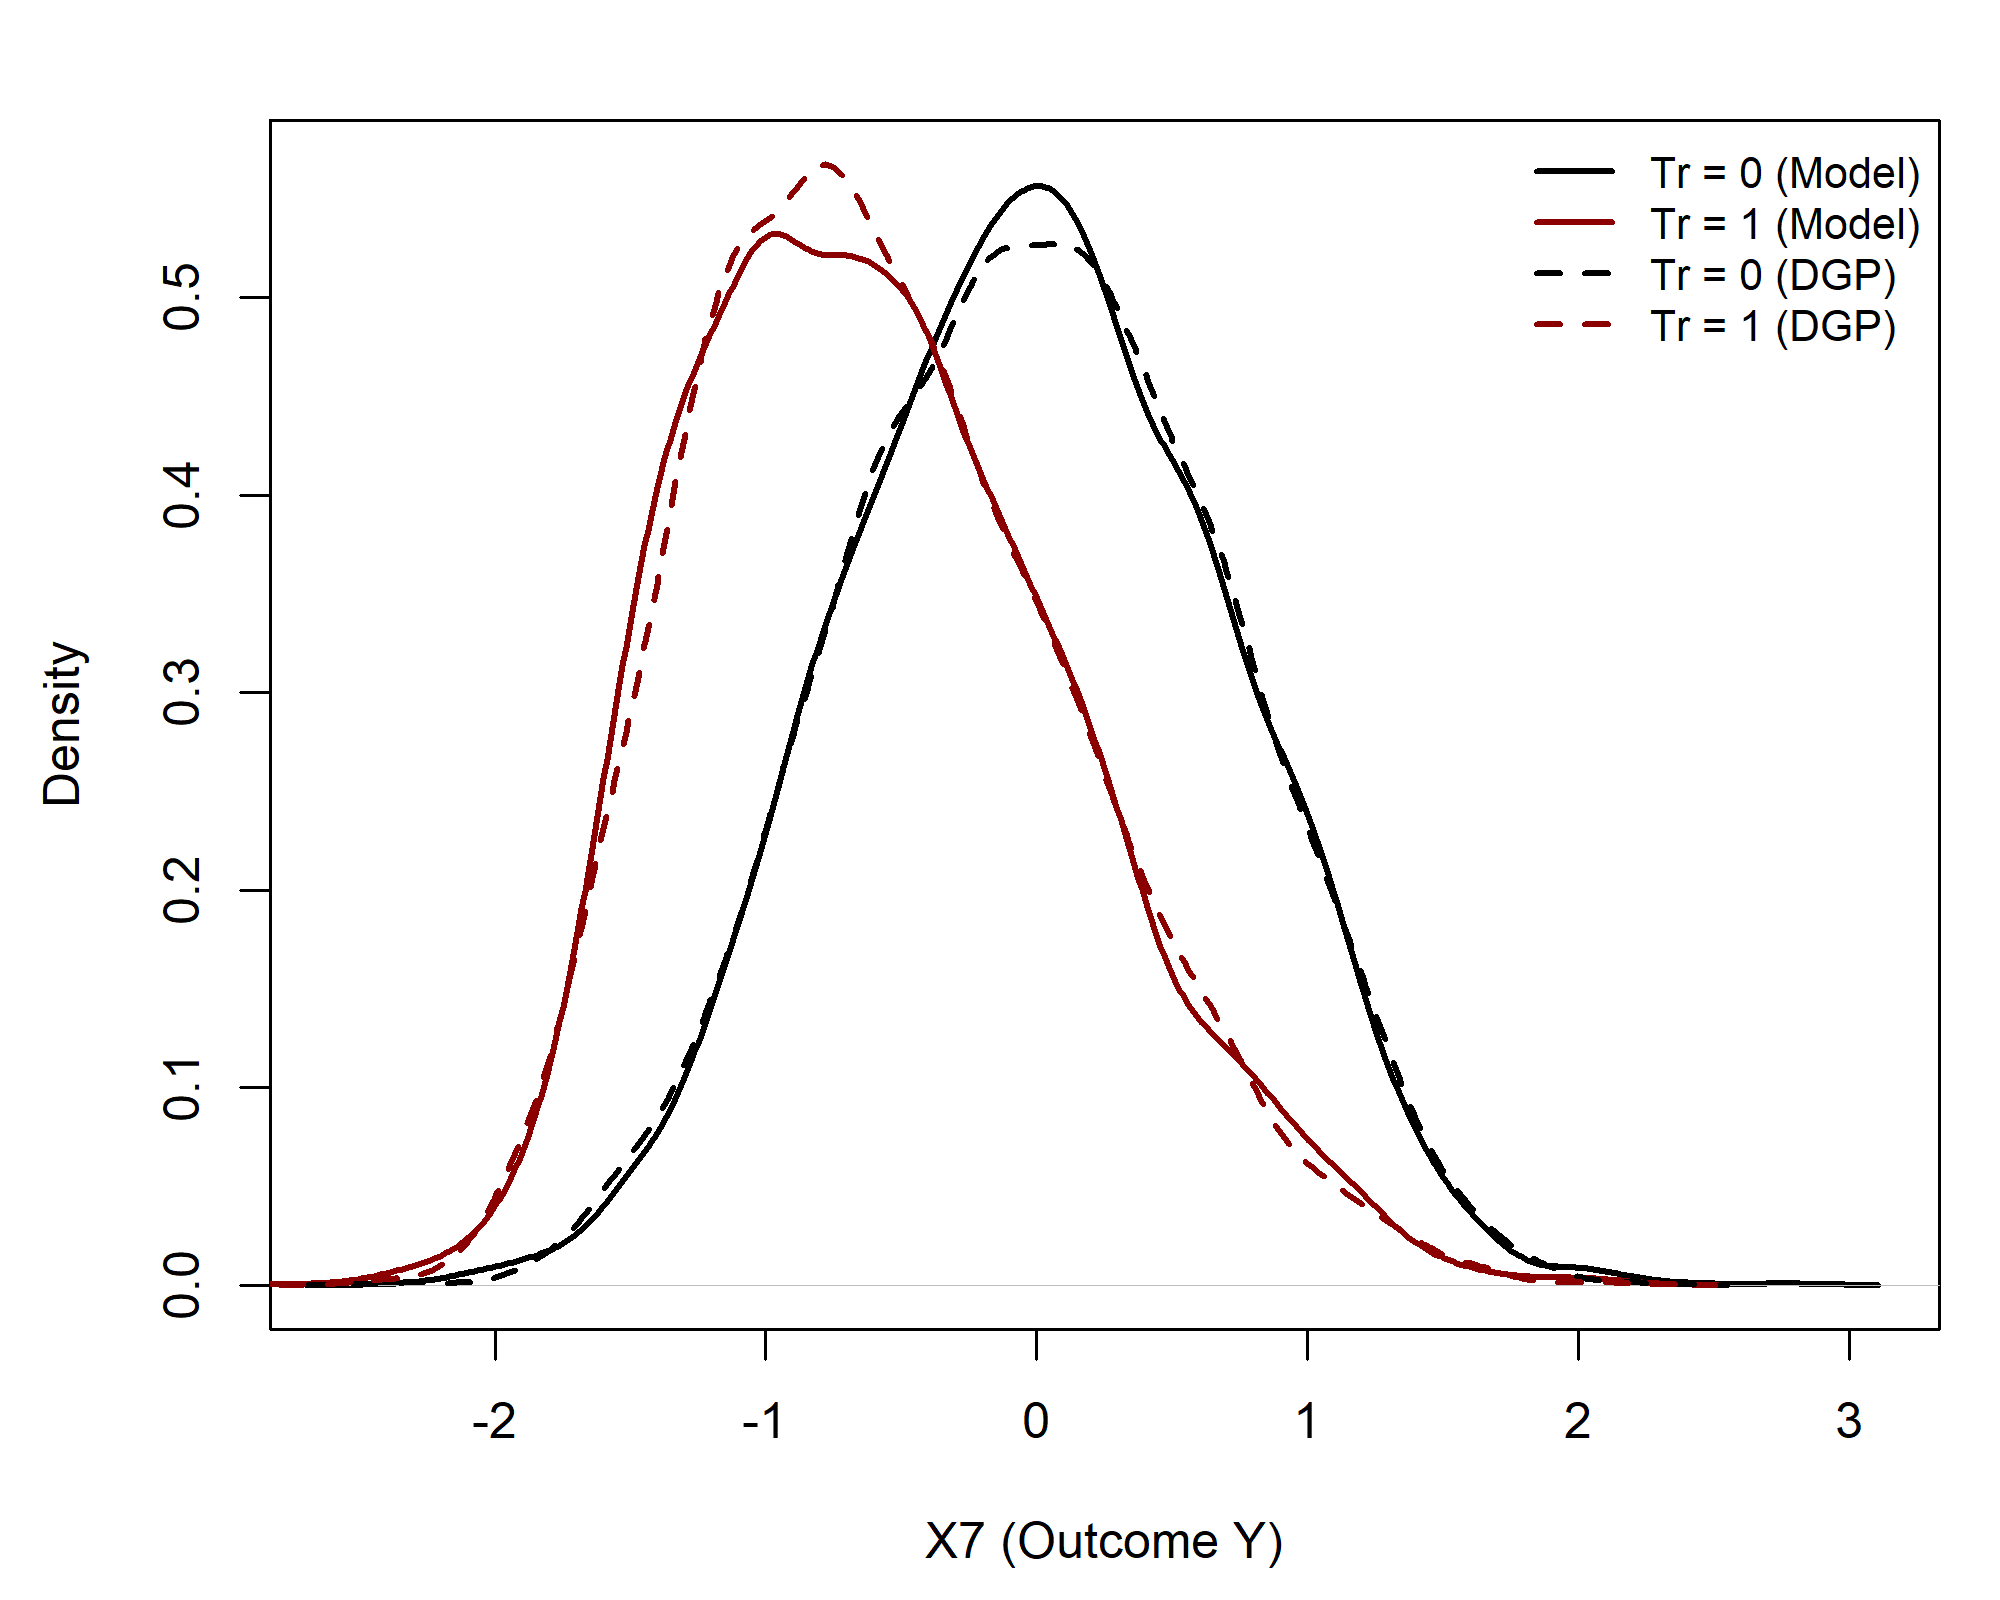
\includegraphics[width=0.45\textwidth]{img/results/observ_scenario1_X7_treatment_densities.png}
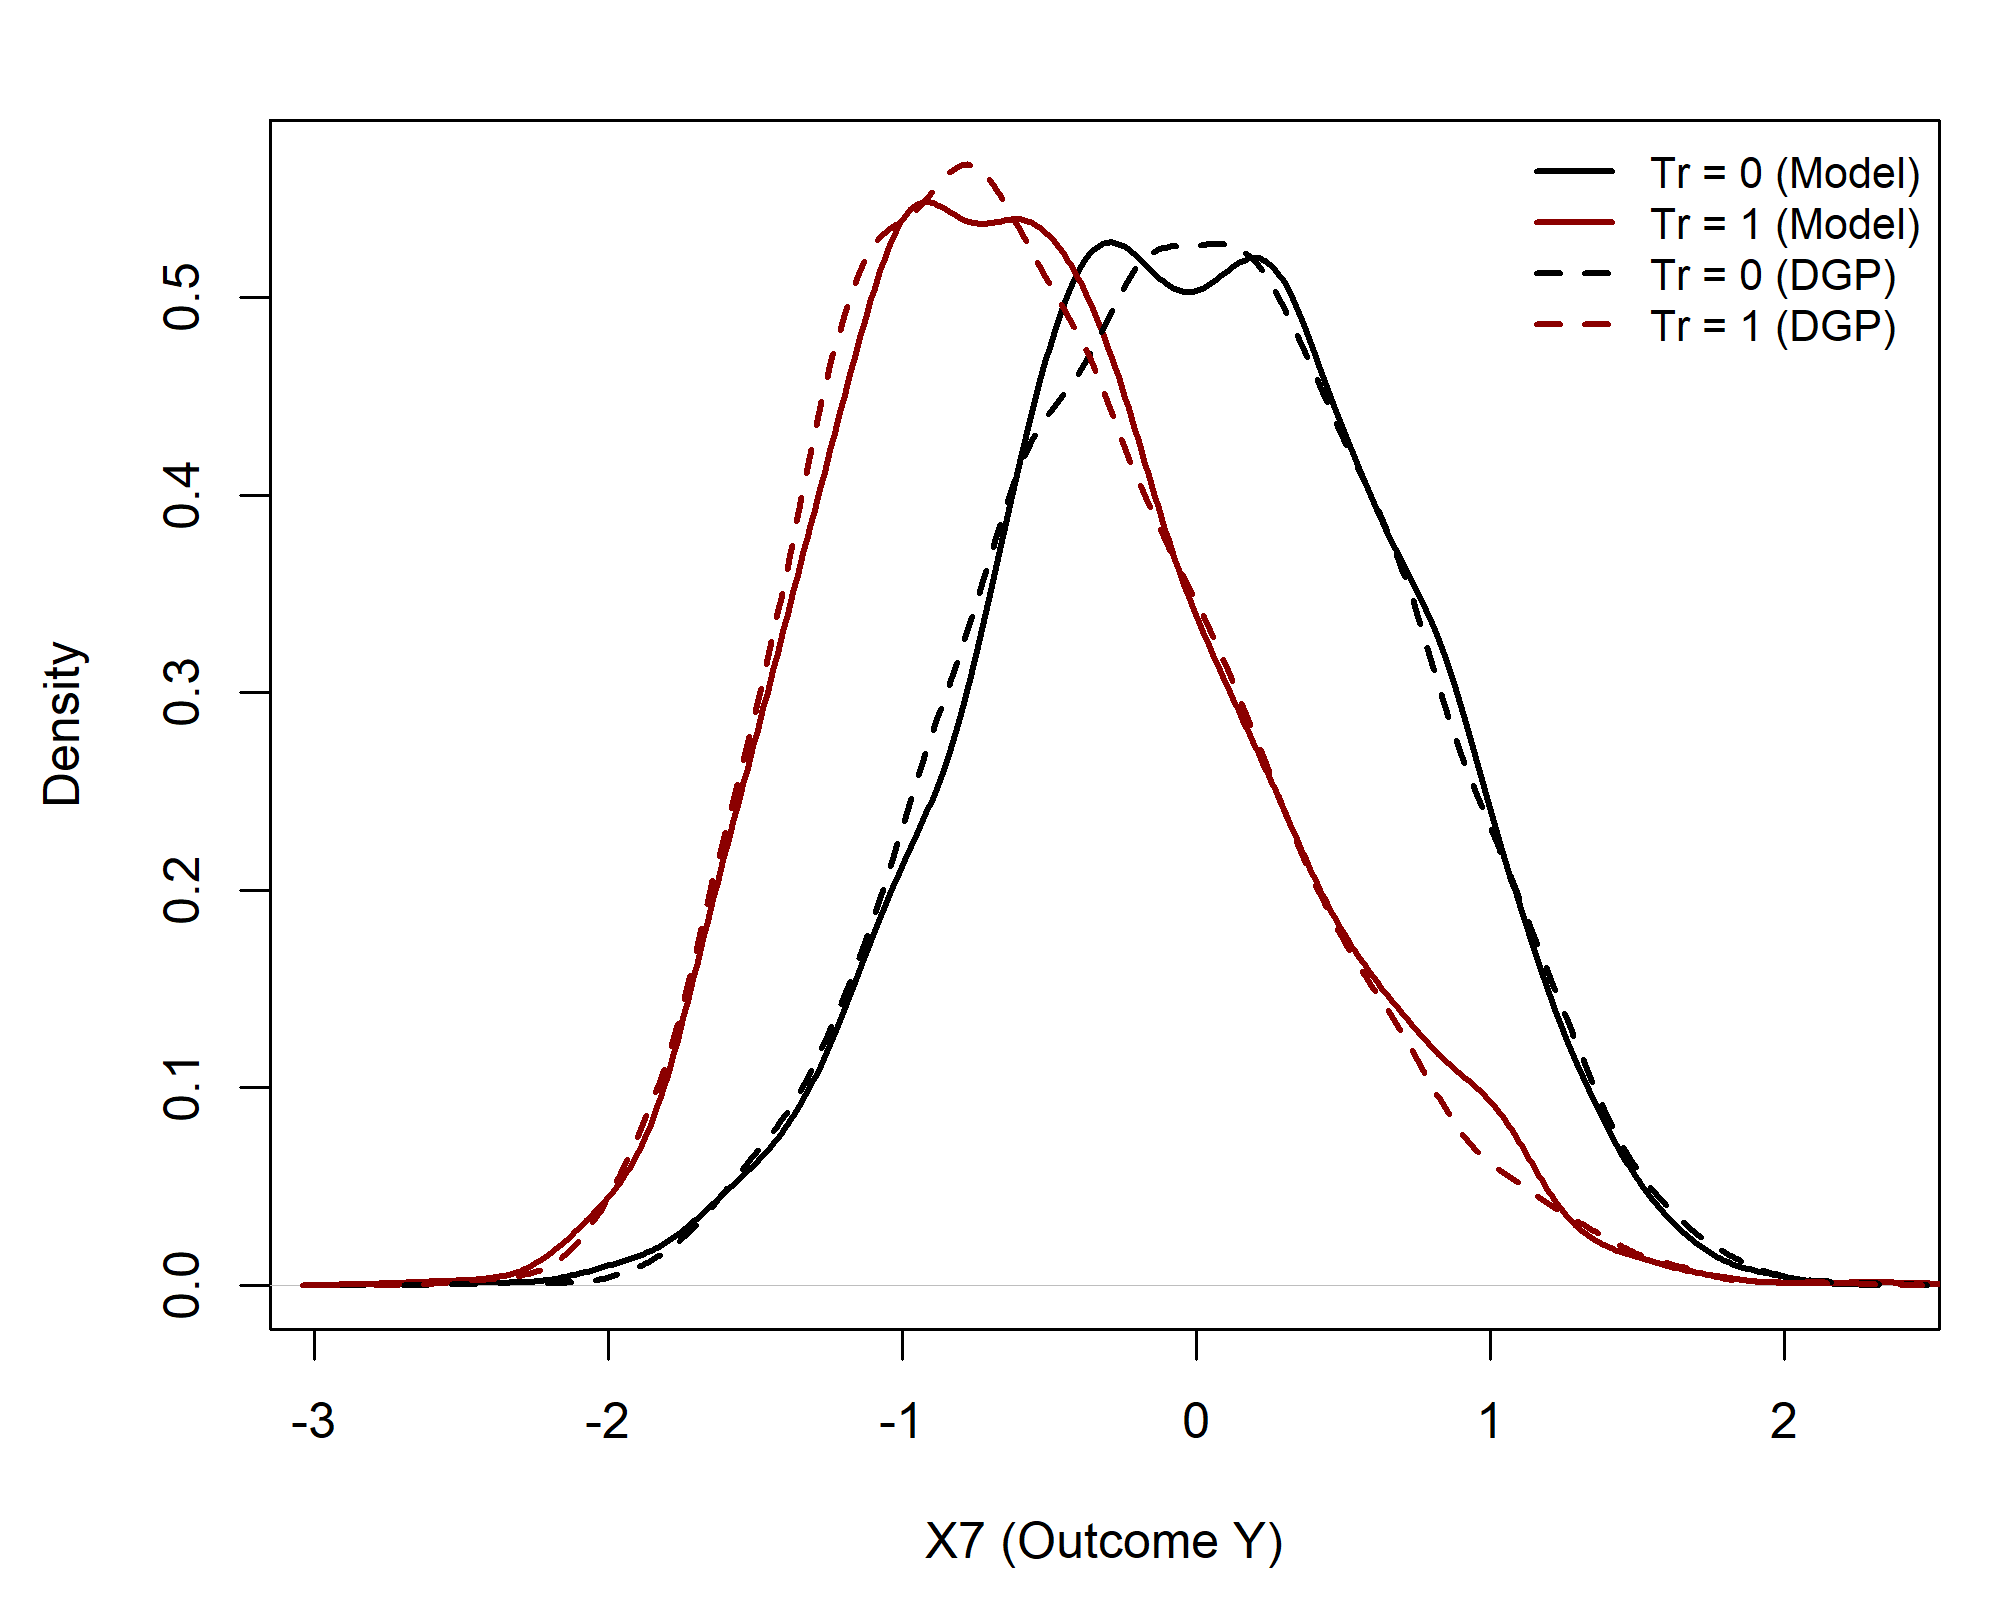
\includegraphics[width=0.45\textwidth]{img/results/rct_scenario1_X7_treatment_densities.png}
\caption{Distributions of the outcome variable ($X_7$) under control and treatment interventions for Scenario (1), which includes both direct and interaction effects. This plot provides a more detailed view of the $X_7$ panels shown under do($X_4=0$) and do($X_4=1$) in Figure~\ref{fig:scenario1_sampling_distributions_vertical}. Left: Observational; Right: RCT setting.}
\label{fig:scenario1_outcome_distributions}
\end{figure}




\begin{figure}[htbp]
\centering
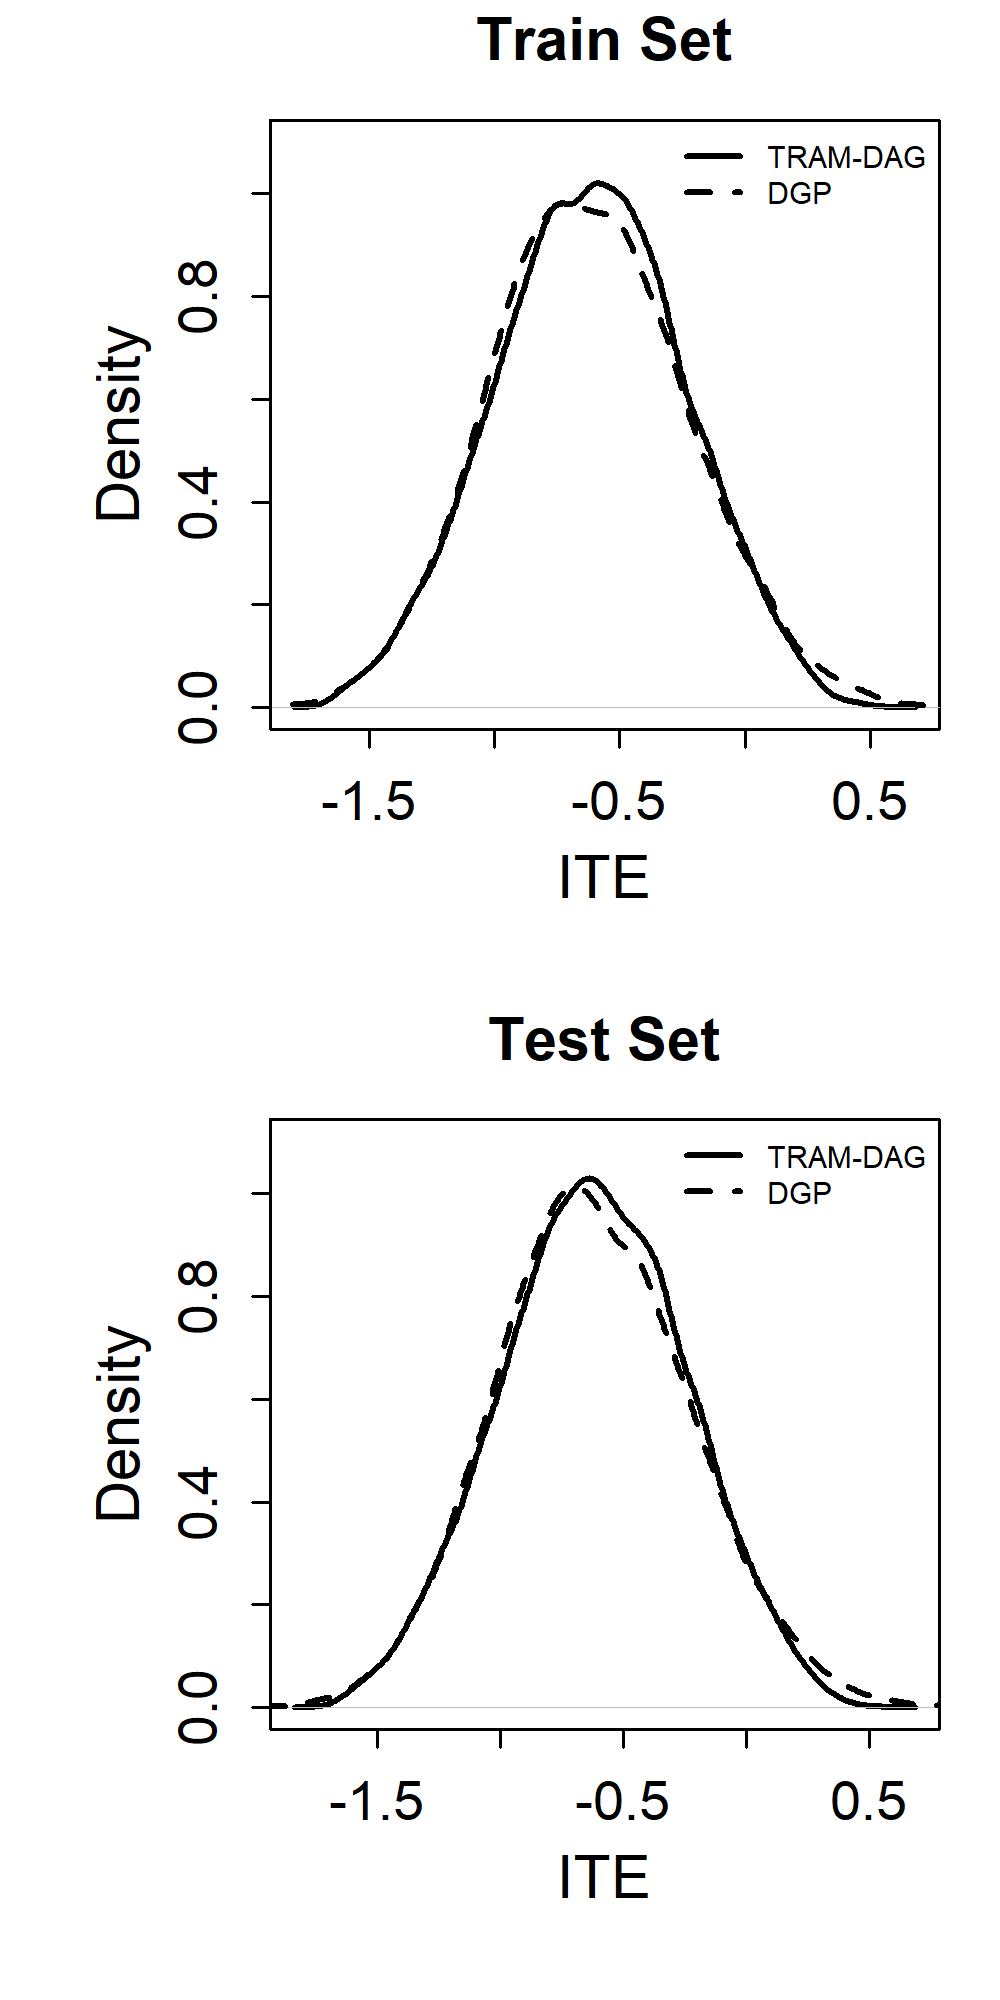
\includegraphics[width=0.33\textwidth]{img/results/observ_scenario1_ITE_densities_train_test.png} 
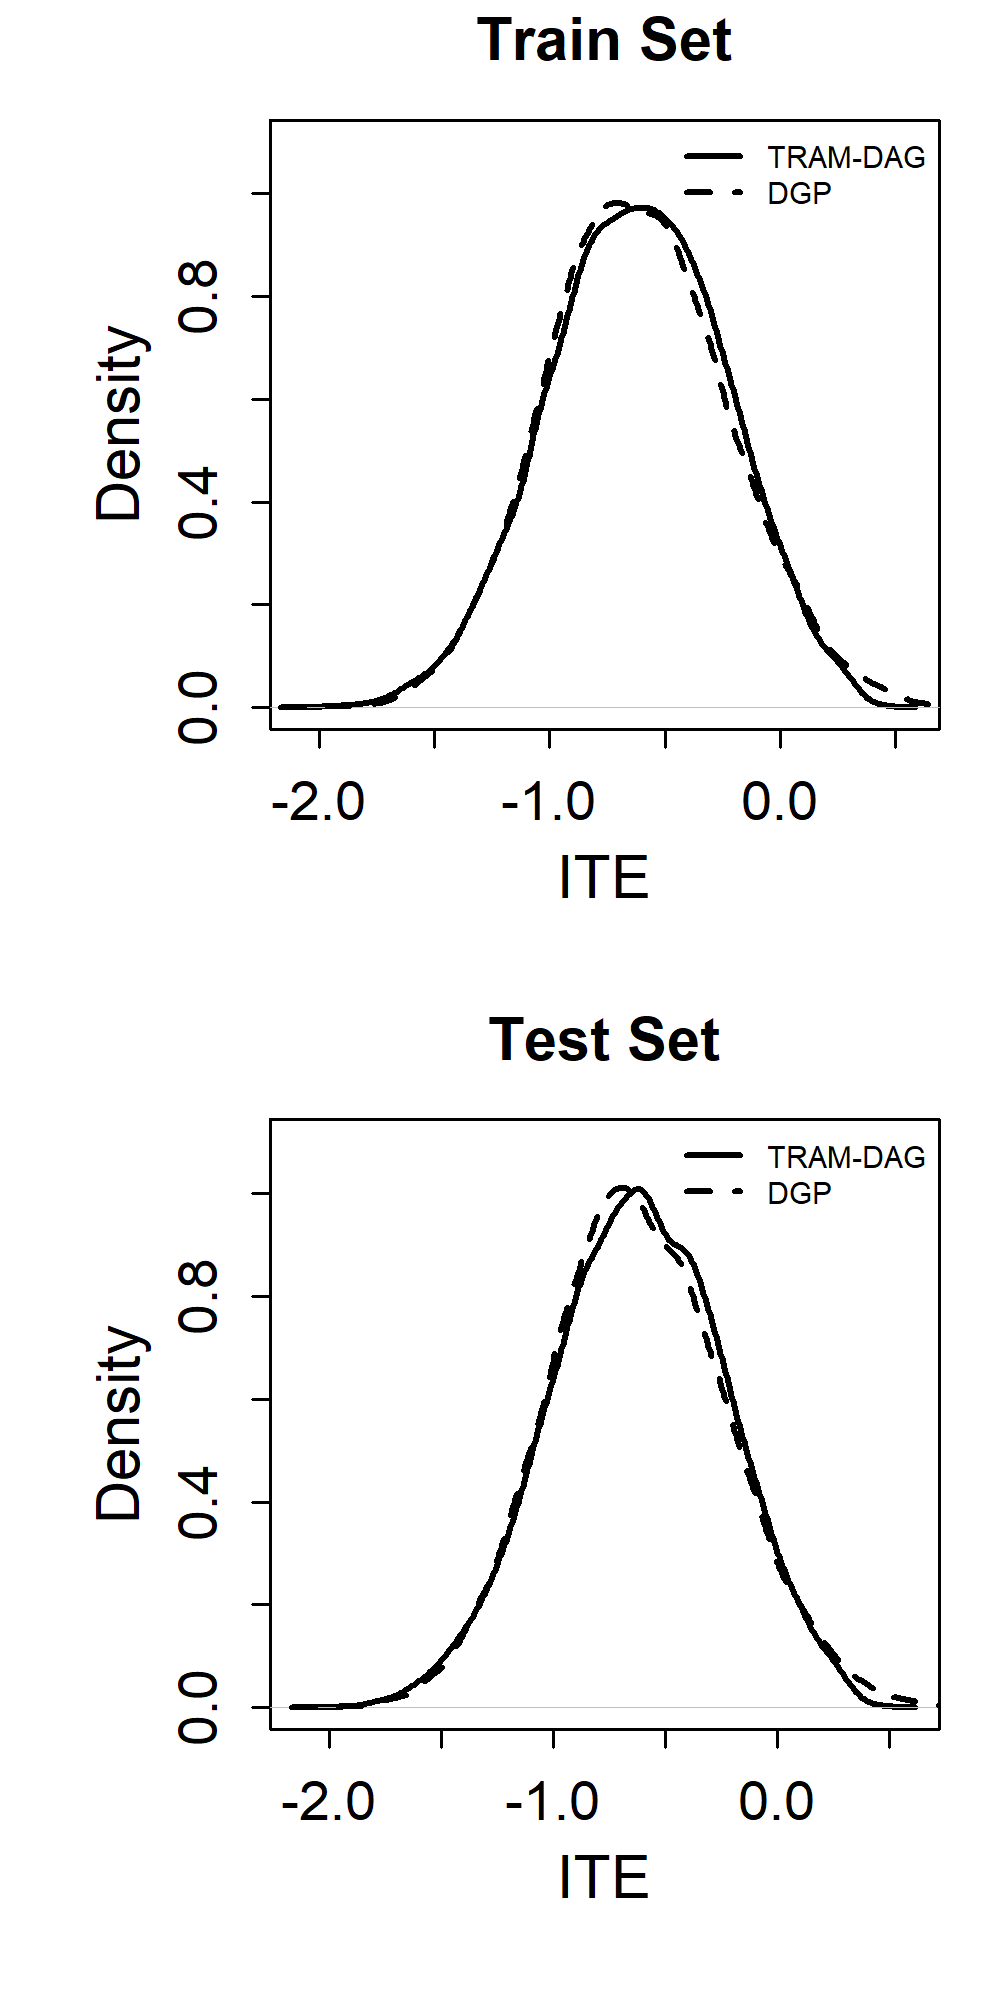
\includegraphics[width=0.33\textwidth]{img/results/rct_scenario1_ITE_densities_train_test.png}
\vspace{-17pt}
\caption{Densities of the estimated ITEs compared to the true ITEs in the training and test datasets for Scenario (1), which includes direct and interaction effects. Left: Observational; Right: RCT setting.}
\label{fig:scenario1_ite_densities_train_test}
\end{figure}






\begin{figure}[htbp]
\centering
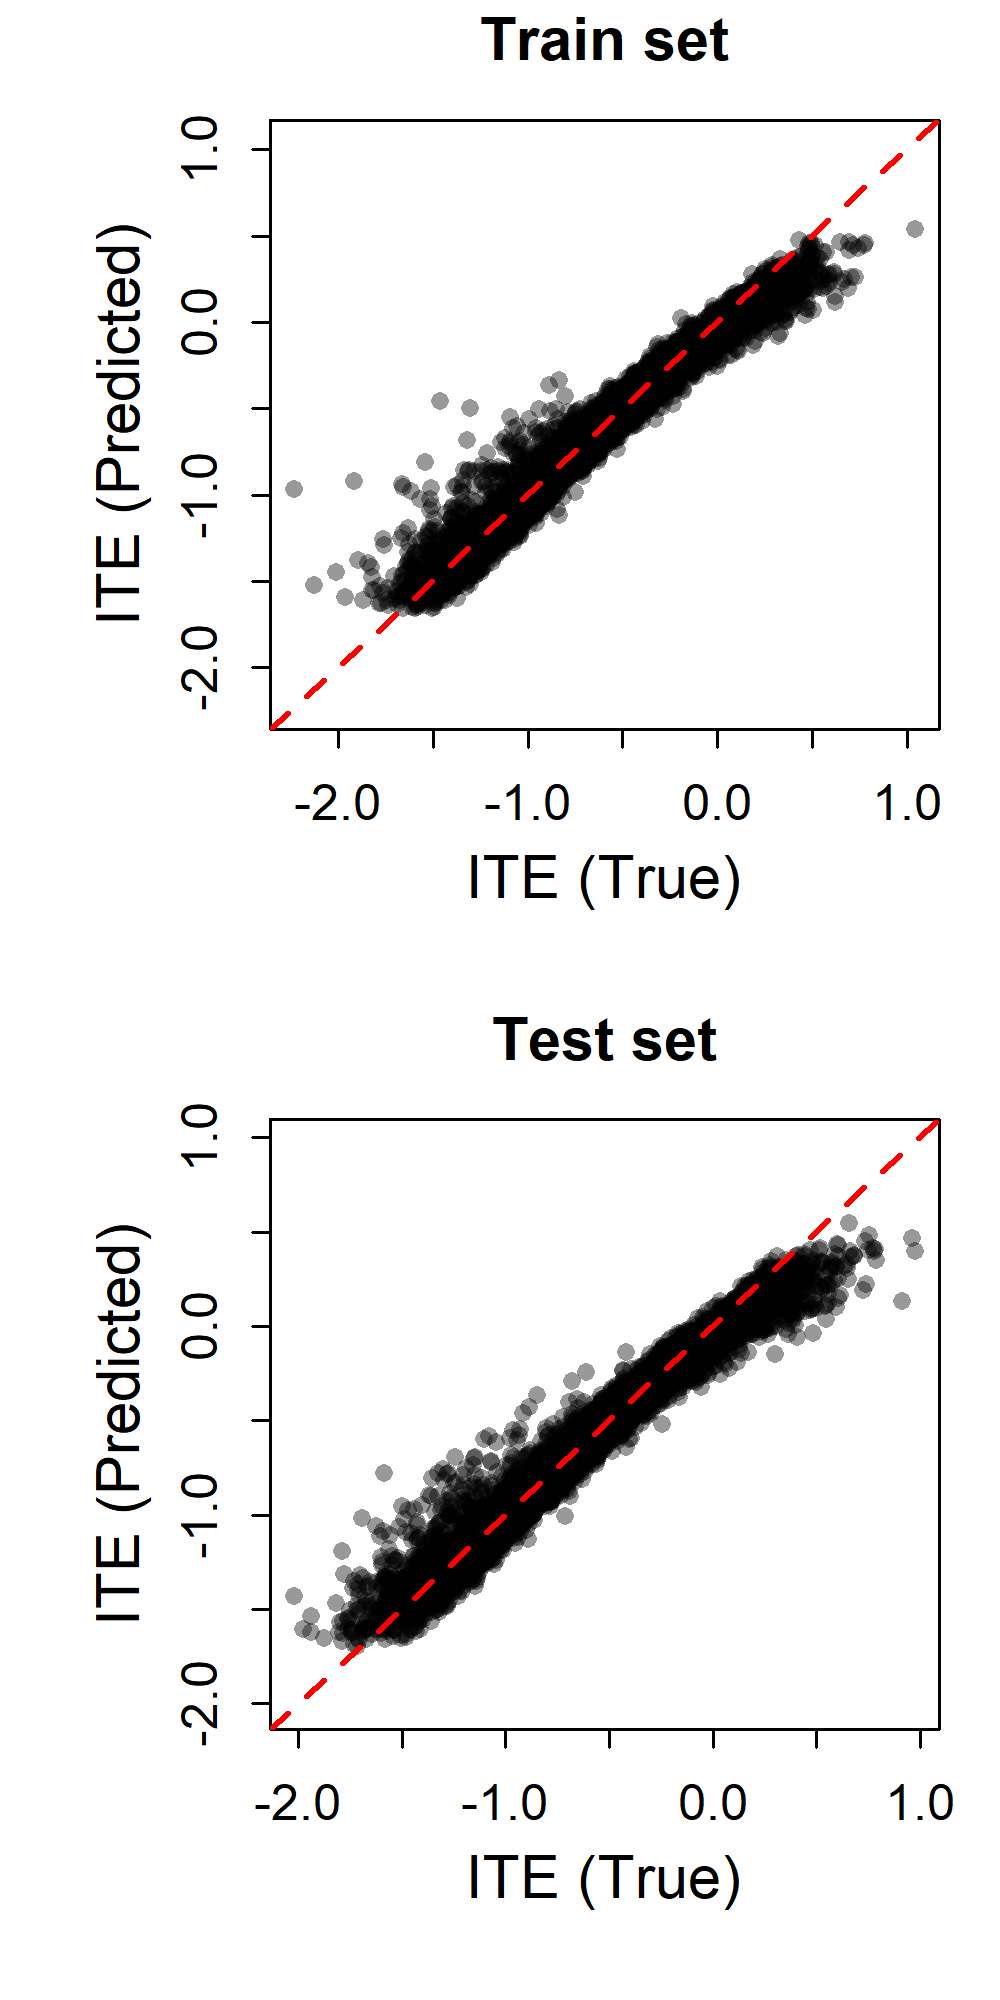
\includegraphics[width=0.33\textwidth]{img/results/observ_scenario1_ITE_scatter_train_test.png} 
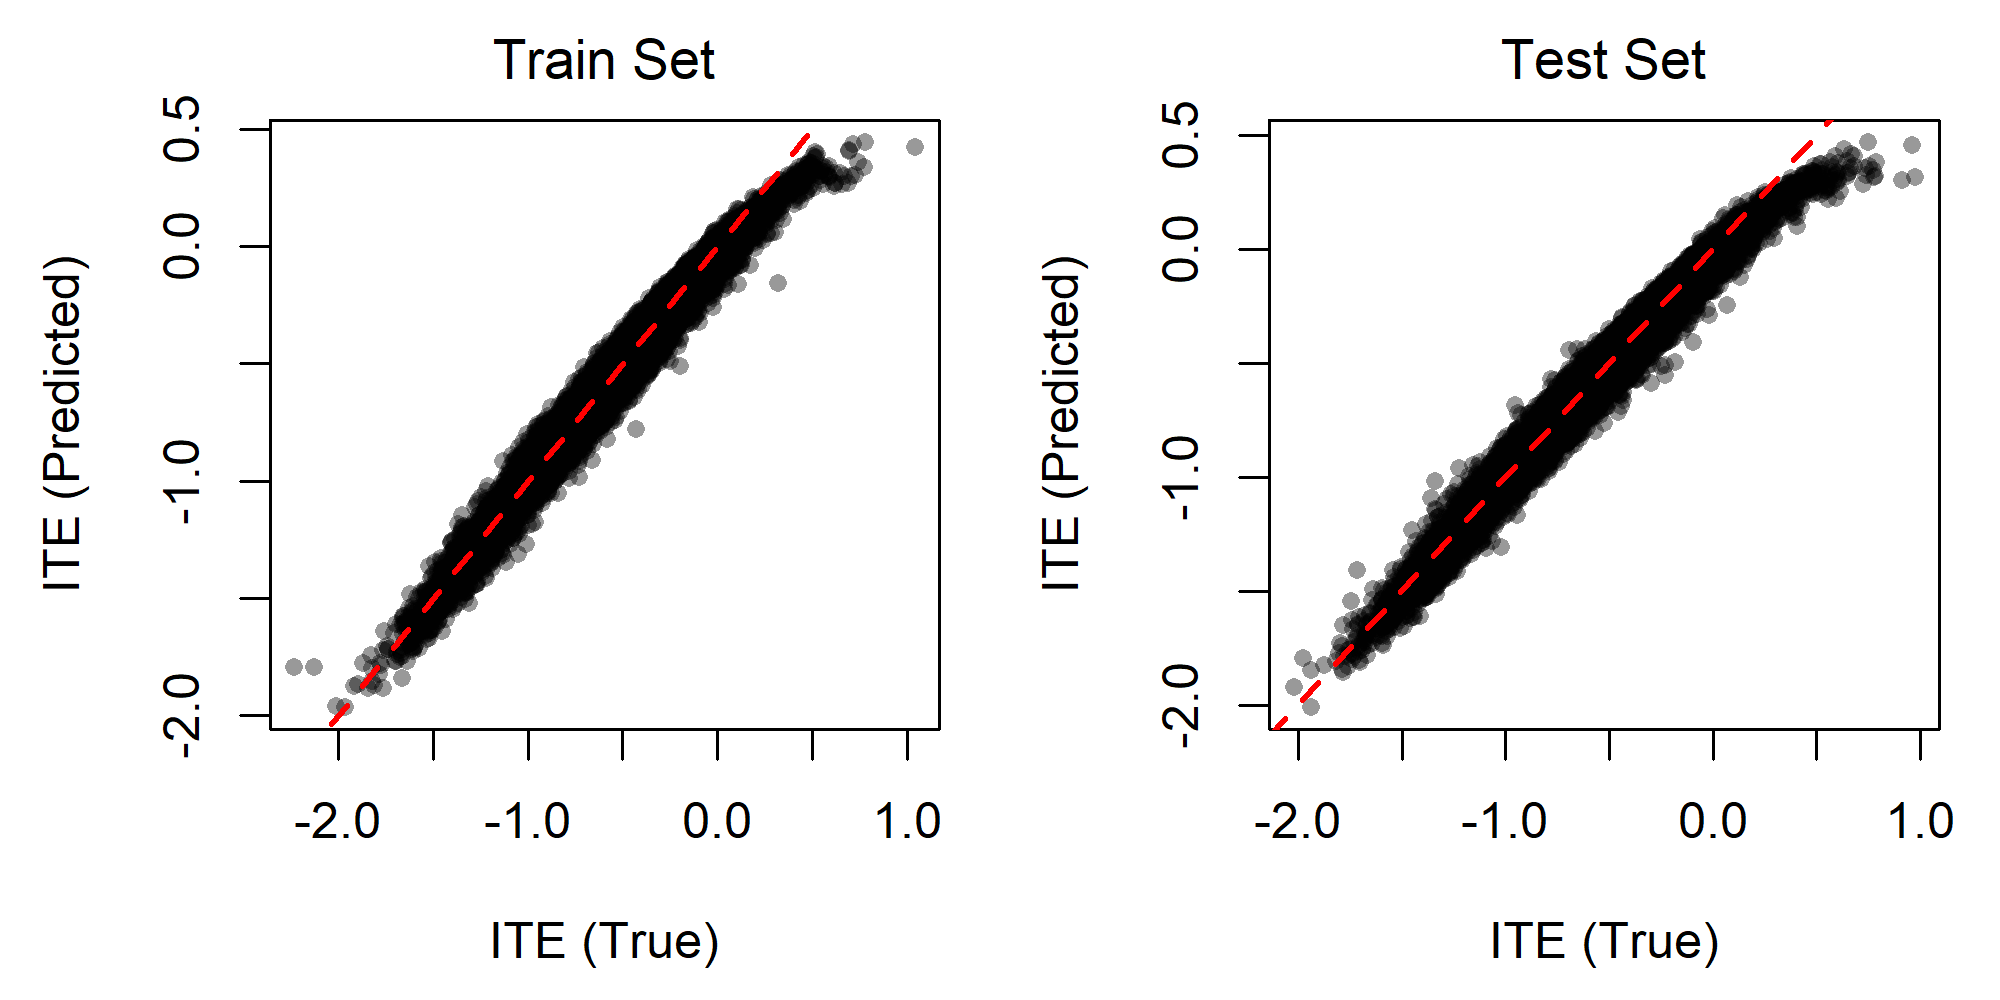
\includegraphics[width=0.33\textwidth]{img/results/rct_scenario1_ITE_scatter_train_test.png}
\vspace{-17pt}
\caption{Scatterplots of estimated ITEs vs. true ITEs in the training and test datasets for Scenario (1), which includes direct and interaction effects. Left: Observational; Right: RCT setting.}
\label{fig:scenario1_ite_scatter_train_test}
\end{figure}



% 
% \begin{figure}[htbp]
% \centering
% 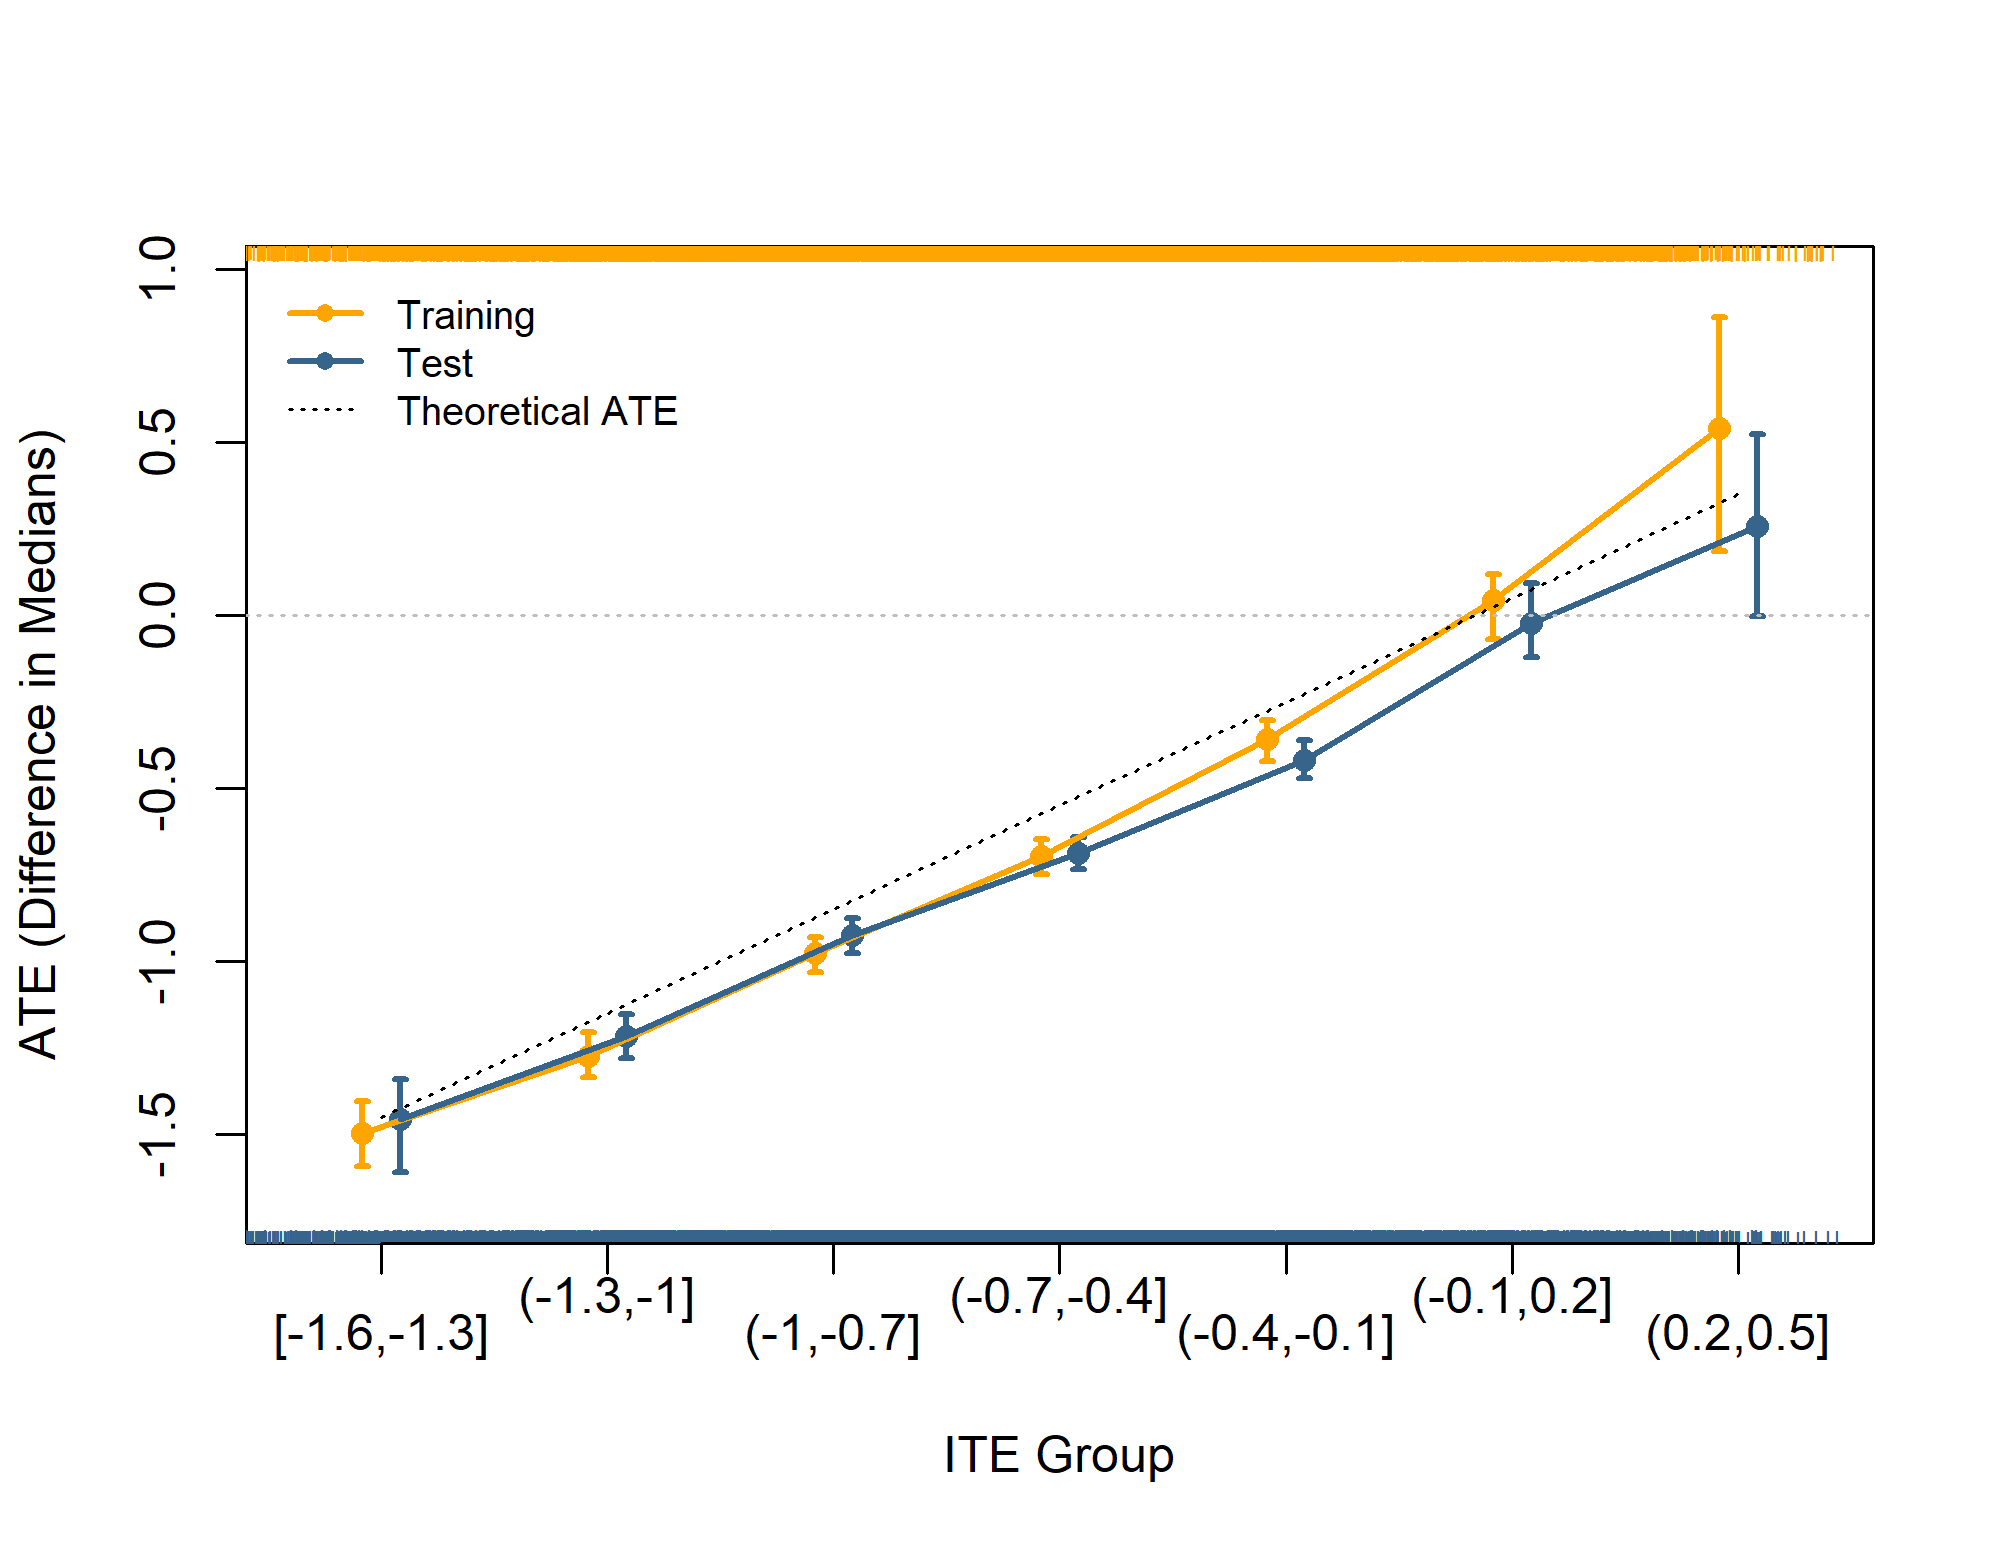
\includegraphics[width=0.45\textwidth]{img/results/observ_scenario1_ITE_ATE.png}
% 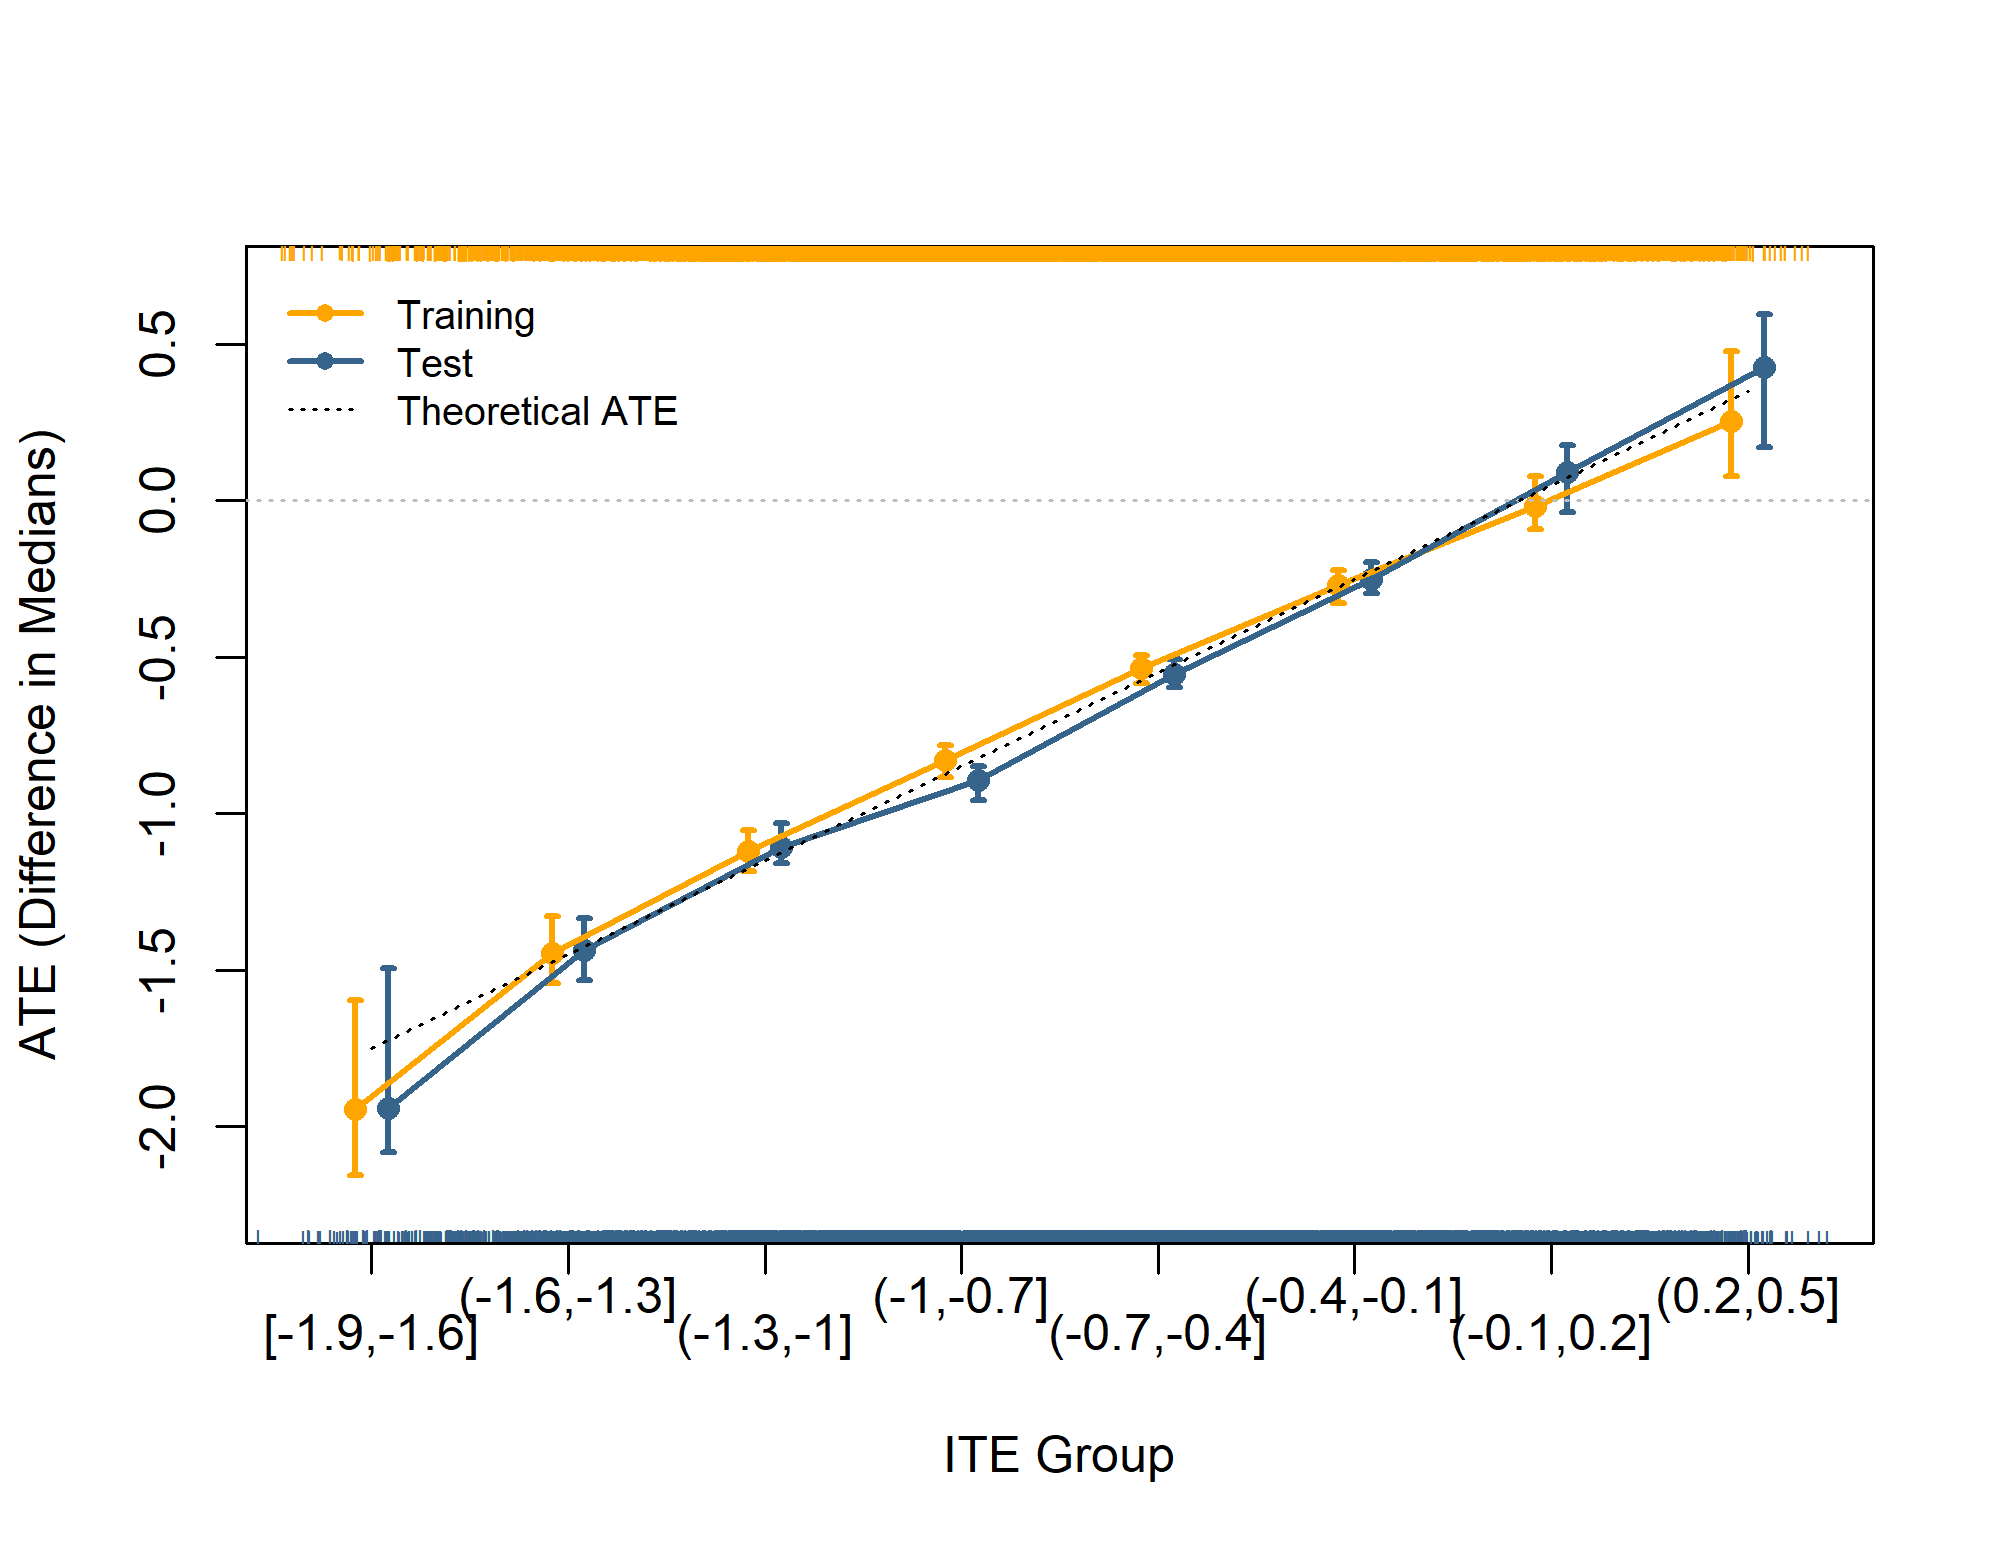
\includegraphics[width=0.45\textwidth]{img/results/rct_scenario1_ITE_ATE.png}
% \caption{ITE-ATE plots for Scenario (1), which includes direct and interaction effects. Individuals are grouped into bins based on their estimated ITEs, and within each bin, the ATE is calculated as the difference in medians of the observed outcomes under the two treatments. 95\% bootstrap confidence intervals indicate the uncertainty. Left: Observational; Right: RCT setting.}
% \label{fig:scenario1_ite_cATE}
% \end{figure}


\begin{figure}[htbp]
\centering
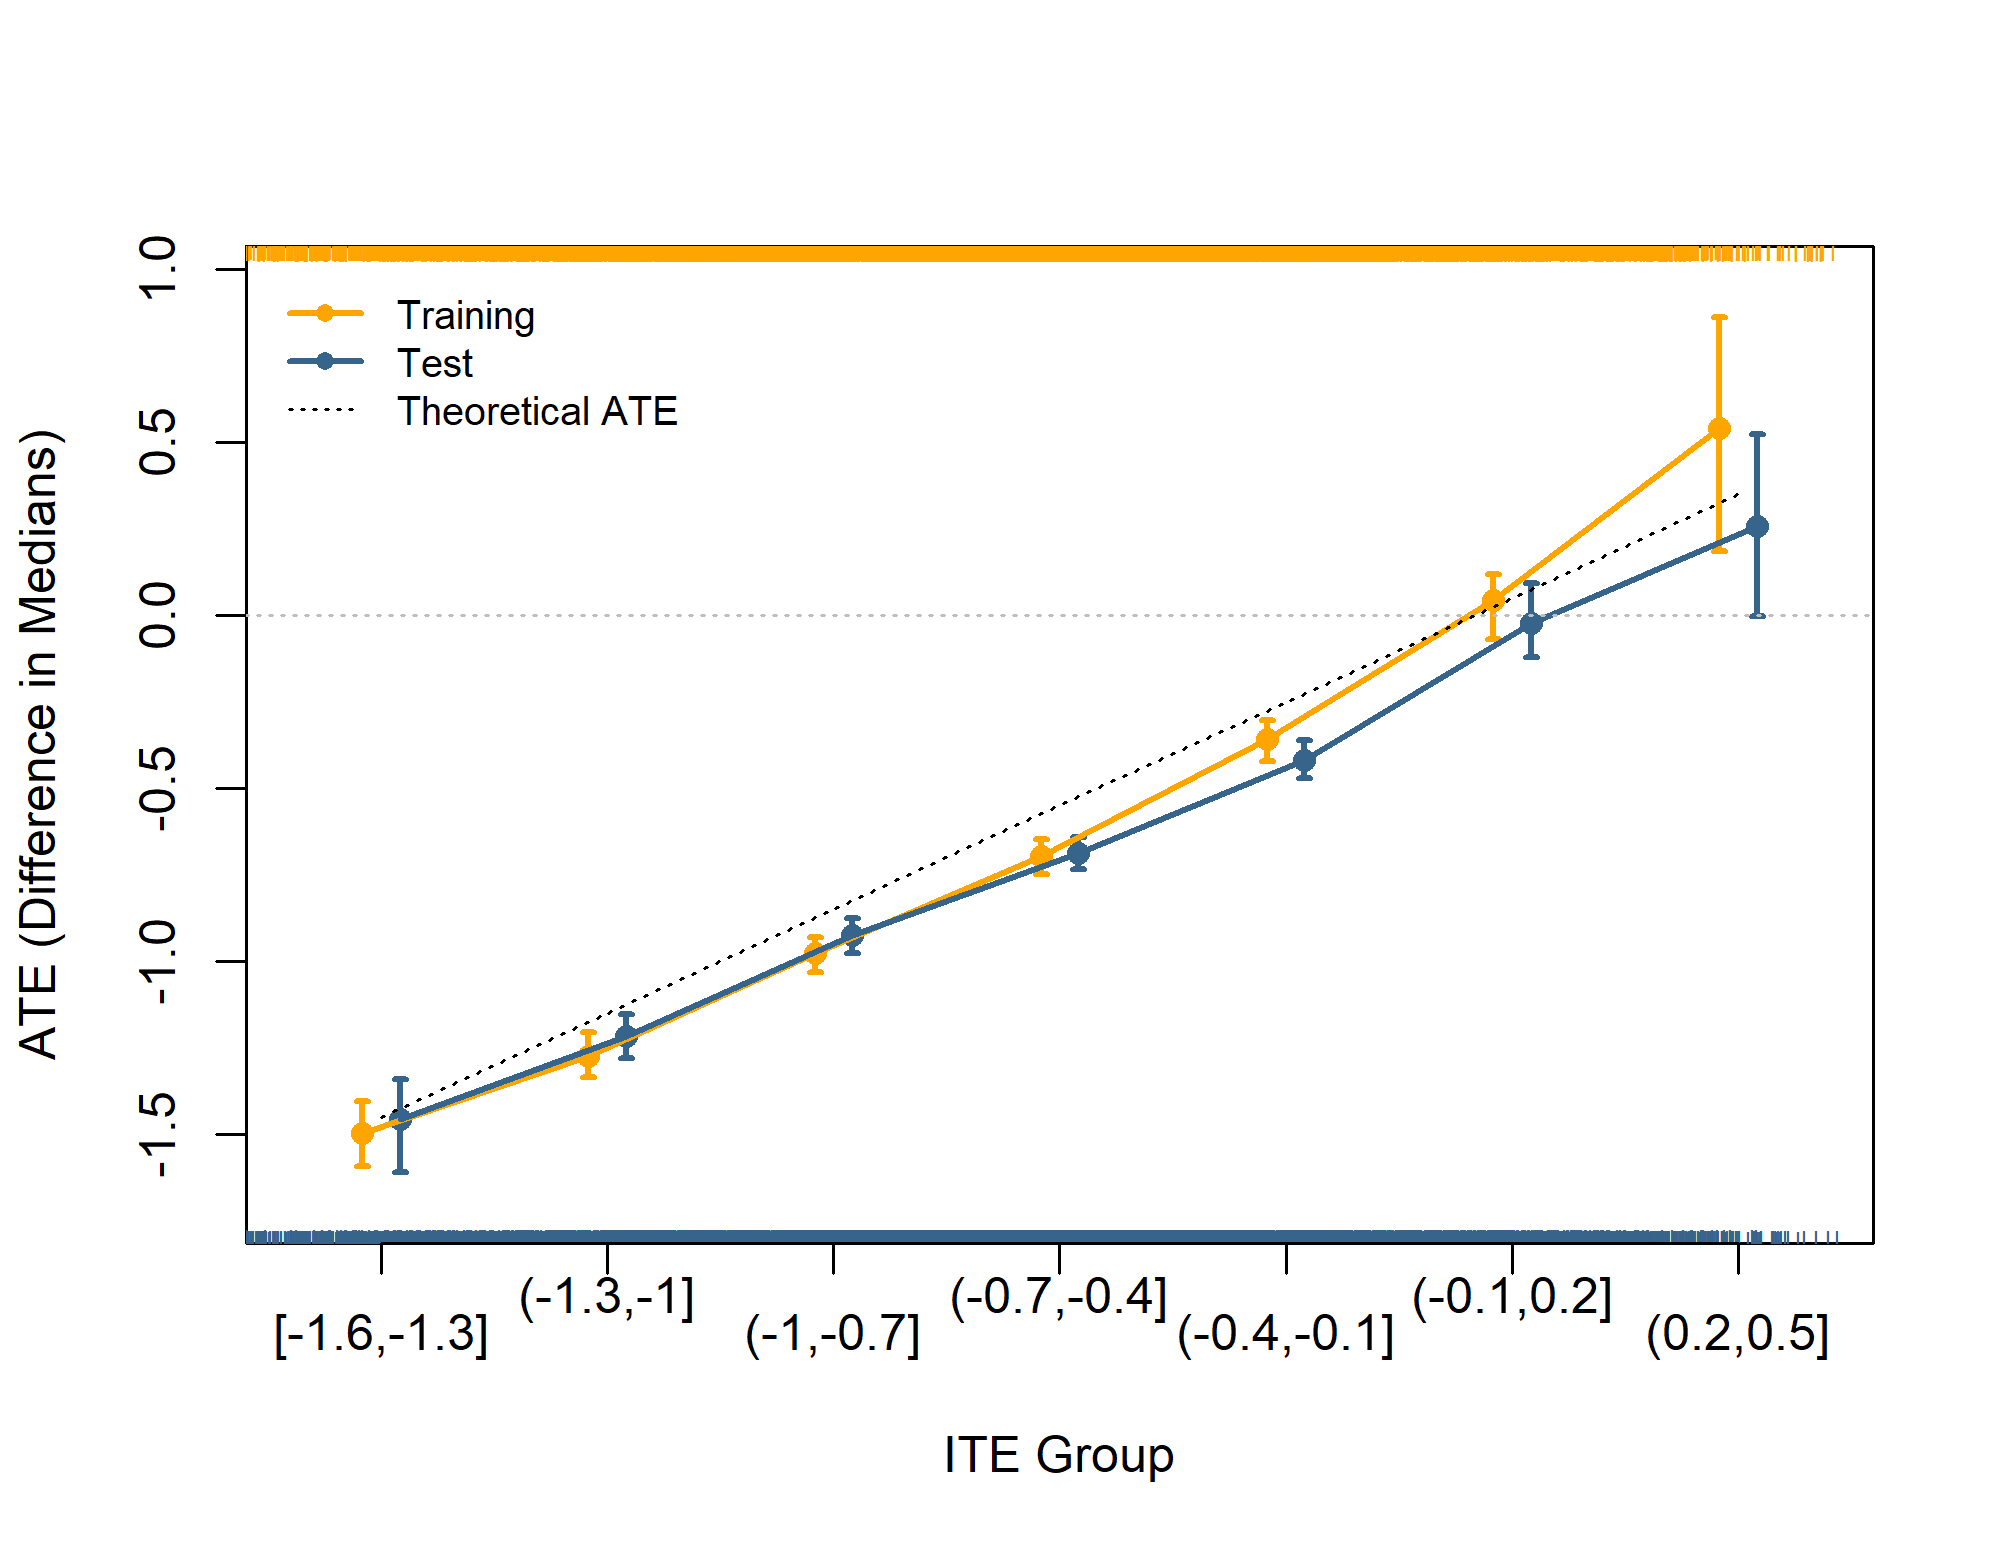
\includegraphics[width=0.8\textwidth]{img/results/observ_scenario1_ITE_ATE.png}
\vspace{-15pt}
\caption{ITE-ATE plot for Scenario (1) in the observatinal setting, which includes direct and interaction effects. Individuals are grouped into bins based on their estimated ITEs, and within each bin, the ATE is calculated as the difference in medians of the observed outcomes under the two treatments. 95\% bootstrap confidence intervals indicate the uncertainty.}
\label{fig:observ_scenario1_ite_ATE}
\end{figure}


\begin{figure}[htbp]
\centering
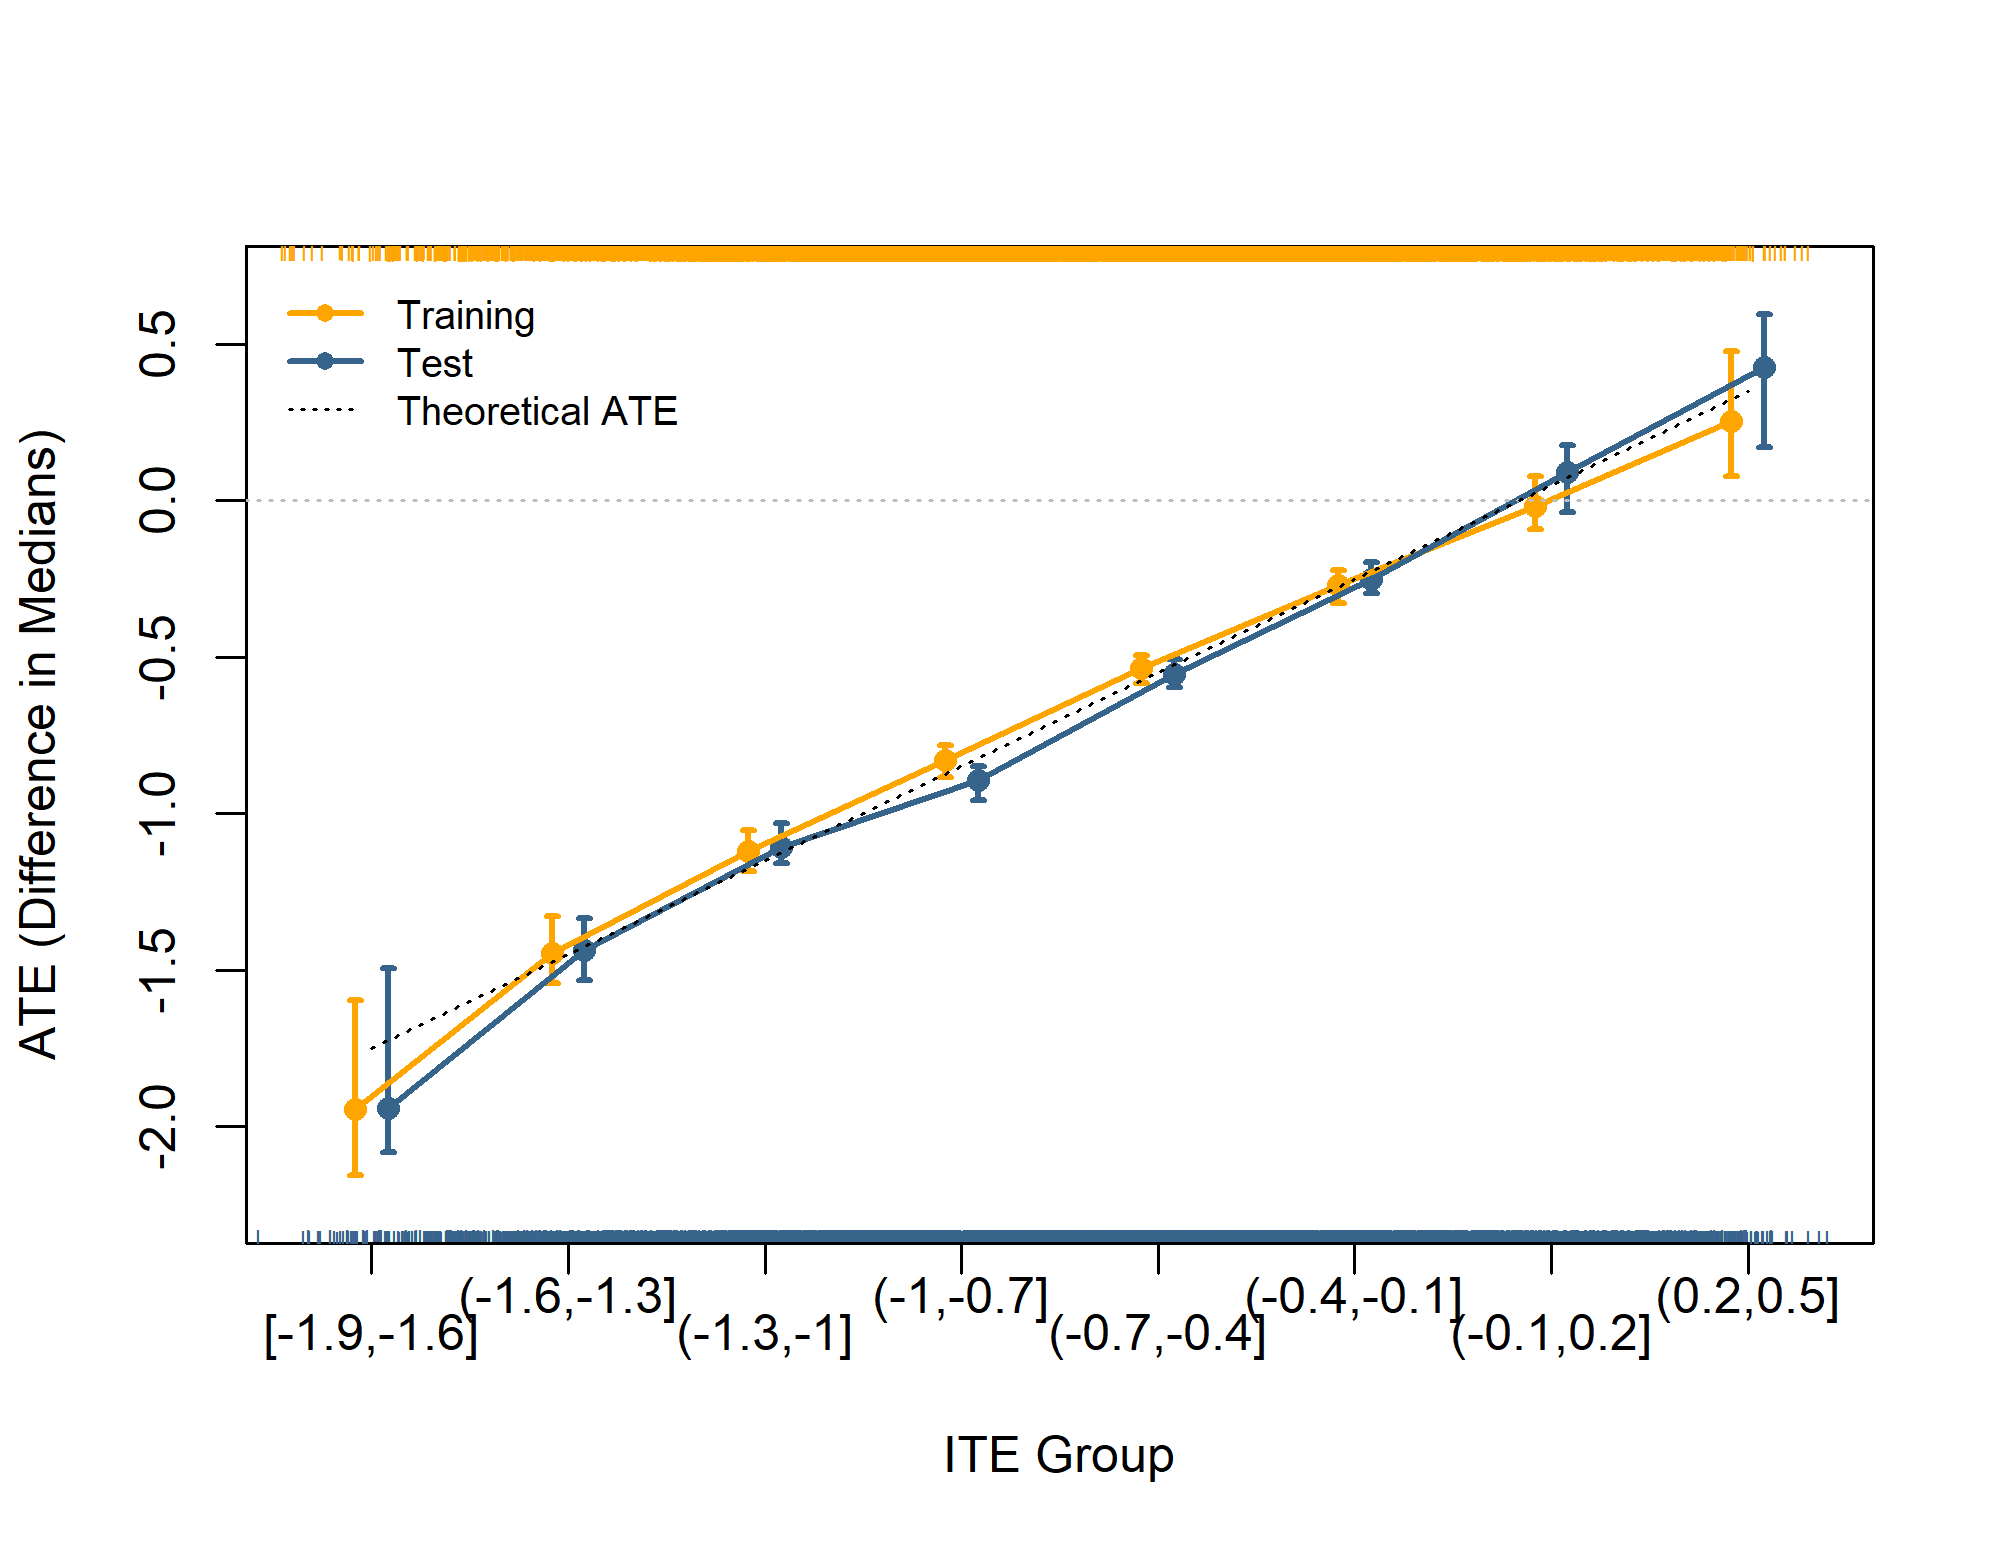
\includegraphics[width=0.8\textwidth]{img/results/rct_scenario1_ITE_ATE.png}
\vspace{-15pt}
\caption{ITE-ATE plot for Scenario (1) in the RCT setting, which includes direct and interaction effects. Individuals are grouped into bins based on their estimated ITEs, and within each bin, the ATE is calculated as the difference in medians of the observed outcomes under the two treatments. 95\% bootstrap confidence intervals indicate the uncertainty.}
\label{fig:rct_scenario1_ite_ATE}
\end{figure}


% start a new page
\clearpage


\subsection{Scenario (2): With direct effect, but no interaction effects}

\begin{figure}[H]
\centering
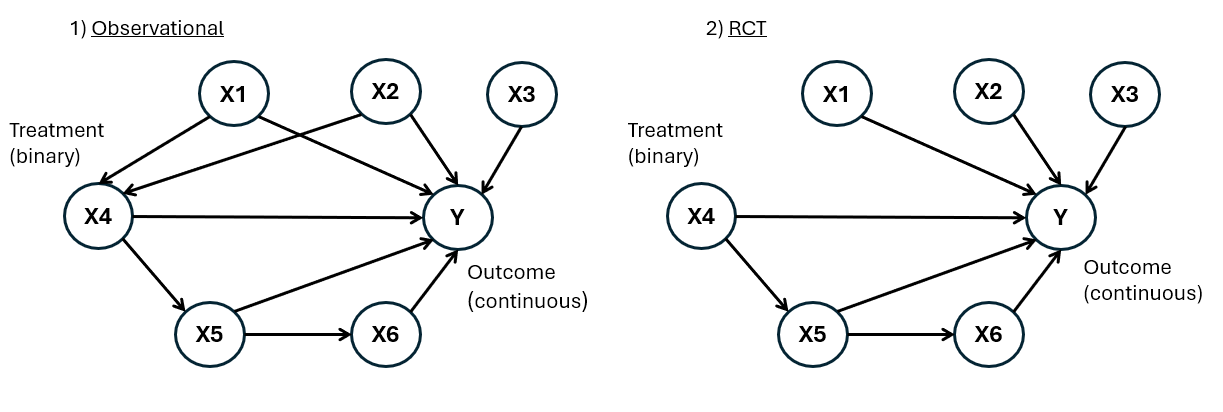
\includegraphics[width=0.85\textwidth]{img/exp4_dag_2.png}
\caption{DAGs for Scenario~(2), which includes a direct effect of the treatment on the outcome, but no interaction effects that would induce treatment effect heterogeneity. Left: Observational setting; Right: RCT setting.}
\label{fig:ite_dag_observational_2}
\end{figure}

Scenario (2) includes a direct effect of the treatment on the outcome, while the coefficients for the interaction terms are set to zero. This results in less heterogeneity in the ITE distribution compared to Scenario (1), as shown in Figure~\ref{fig:scenario2_ite_distribution_dgp}. Why there is still some heterogeneity despite the absence of interactions is discussed in Section~\ref{sec:disc_experiment4}. The observational and interventional densities generated by the fitted TRAM-DAG closely match the true densities defined by the DGP, as illustrated in Figures~\ref{fig:scenario2_sampling_distributions_vertical} and~\ref{fig:scenario2_outcome_distributions}. However, there is a notable difference in variance between the estimated and true ITE distributions, visible in Figures~\ref{fig:scenario2_ite_densities_train_test} and~\ref{fig:scenario2_ite_scatter_train_test}. The ITE-ATE plots in Figures~\ref{fig:observ_scenario2_ite_ATE} and \ref{fig:rct_scenario2_ite_ATE} are less informative than in Scenario (1), as expected given the reduced heterogeneity. Table~\ref{tab:scenario2_ate_comparison} presents the ATE measures for Scenario (2). In the test set of the RCT setting, the ATE based on the true ITEs was -0.633, while the ATE based on the estimated ITEs was -0.586.


\begin{table}[htbp]
\centering
\small
\caption{Scenario (2), including a direct treatment effect but no interaction effects: Comparison of ATE measures across train and test sets for the observational and RCT setting. $\text{Y}_\text{observed}^{(\text{Tr})}$ denotes the observed outcome under the treatment ($\text{Tr}$) actually received. The estimated ATE from $\text{mean}(\text{ITE}_\text{estimated})$ can be directly compared to the true $\text{mean}(\text{ITE}_\text{true})$, whereas comparisons to the empirical ATEs based on outcome differences should be interpreted with caution.}
\label{tab:scenario2_ate_comparison}
\begin{tabular}{l c c c c}
\toprule
\textbf{Measure} & \multicolumn{2}{c}{\textbf{Observational}} & \multicolumn{2}{c}{\textbf{RCT}} \\
\cmidrule(lr){2-3} \cmidrule(lr){4-5}
 & \textbf{Train} & \textbf{Test} & \textbf{Train} & \textbf{Test} \\
\midrule
ATE as $\text{mean}(\text{Y}_\text{observed}^{(1)}) - \text{mean}(\text{Y}_\text{observed}^{(0)})$ 
& NA & NA 
& -0.569 
& -0.572 \\

ATE as $\text{median}(\text{Y}_\text{observed}^{(1)}) - \text{median}(\text{Y}_\text{observed}^{(0)})$  
& NA & NA 
& -0.629 
& -0.639 \\

ATE as mean(ITE$_\text{true}$)  
& -0.633 
& -0.633 
& -0.633 
& -0.633 \\

ATE as mean(ITE$_\text{estimated}$) 
& -0.645 
& -0.644 
& -0.587 
& -0.586 \\
\bottomrule
\end{tabular}
\end{table}

% 
% \begin{table}[htbp]
% \centering
% \small
% \caption{Scenario (2), including a direct treatment but no interaction effects: Comparison of ATE measures across train and test sets for the observational and RCT setting.}
% \label{tab:scenario2_ate_comparison_old}
% \begin{tabular}{l c c c c}
% \toprule
% \textbf{Measure} & \multicolumn{2}{c}{\textbf{Observational}} & \multicolumn{2}{c}{\textbf{RCT}} \\
% \cmidrule(lr){2-3} \cmidrule(lr){4-5}
%  & \textbf{Train} & \textbf{Test} & \textbf{Train} & \textbf{Test} \\
% \midrule
% ATE as $\text{mean}(\text{Y}_\text{observed}^{(1)}) - \text{mean}(\text{Y}_\text{observed}^{(0)})$ & NA & NA & round(rct_scenario2$dev_ATE_observed_Y_mean_diff, 3) & round(rct_scenario2$val_ATE_observed_Y_mean_diff, 3) \\
% ATE as $\text{median}(\text{Y}_\text{observed}^{(1)}) - \text{median}(\text{Y}_\text{observed}^{(0)})$  & NA & NA & round(rct_scenario2$dev_ATE_observed_Y_median_diff, 3) & round(rct_scenario2$val_ATE_observed_Y_median_diff, 3) \\
% ATE as mean(ITE$_\text{true}$)  & round(observ_scenario2$dev_ITE_median_average, 3) & round(observ_scenario2$val_ITE_median_average, 3) & round(rct_scenario2$dev_ITE_median_average, 3) & round(rct_scenario2$val_ITE_median_average, 3) \\
% ATE as mean(ITE$_\text{estimated}$) & round(observ_scenario2$dev_ITE_median_pred_average, 3) & round(observ_scenario2$val_ITE_median_pred_average, 3) & round(rct_scenario2$dev_ITE_median_pred_average, 3) & round(rct_scenario2$val_ITE_median_pred_average, 3) \\
% \bottomrule
% \end{tabular}
% \end{table}



\begin{figure}[htbp]
\centering
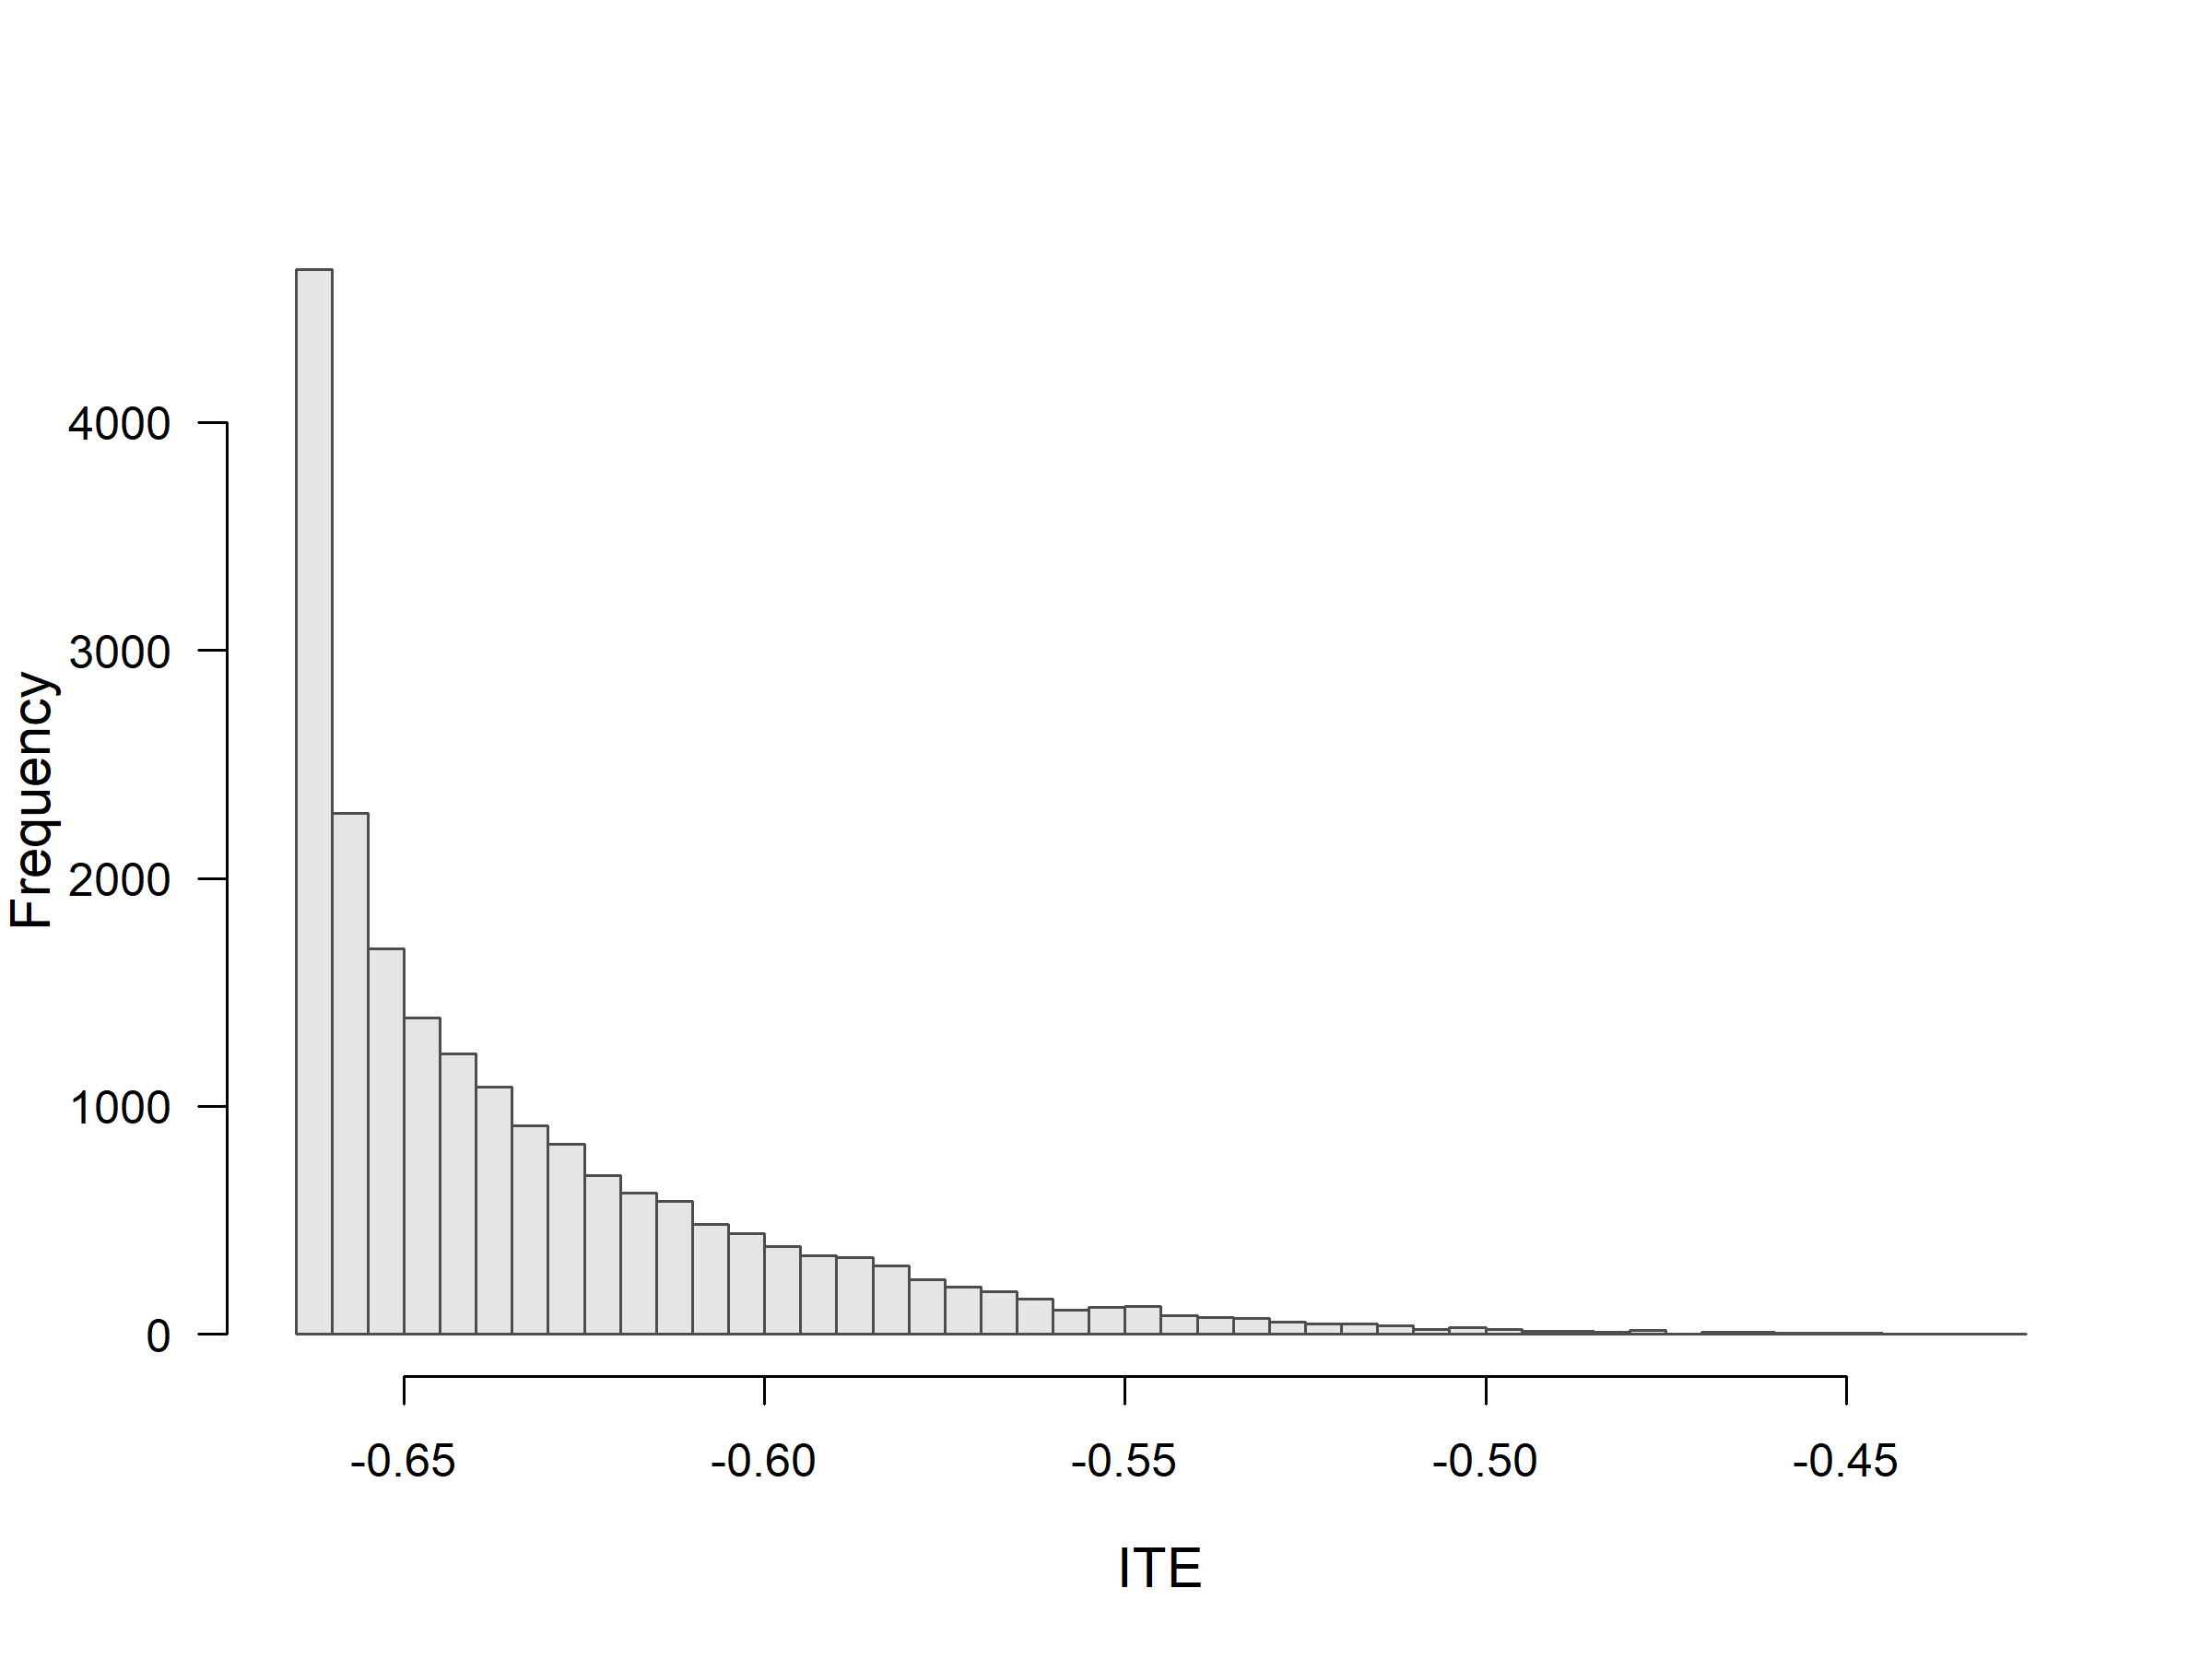
\includegraphics[width=0.7\textwidth]{img/results/observ_scenario2_ite_distribution_dgp.png}
\caption{True ITE distribution resulting from the DGP for Scenario~(2), which includes a direct treatment effect but no interaction effects. The true ITEs are identical in the observational and RCT settings, as they depend only on the potential outcomes under both treatment allocations.}
\label{fig:scenario2_ite_distribution_dgp}
\end{figure}



\begin{figure}[htbp]
\centering
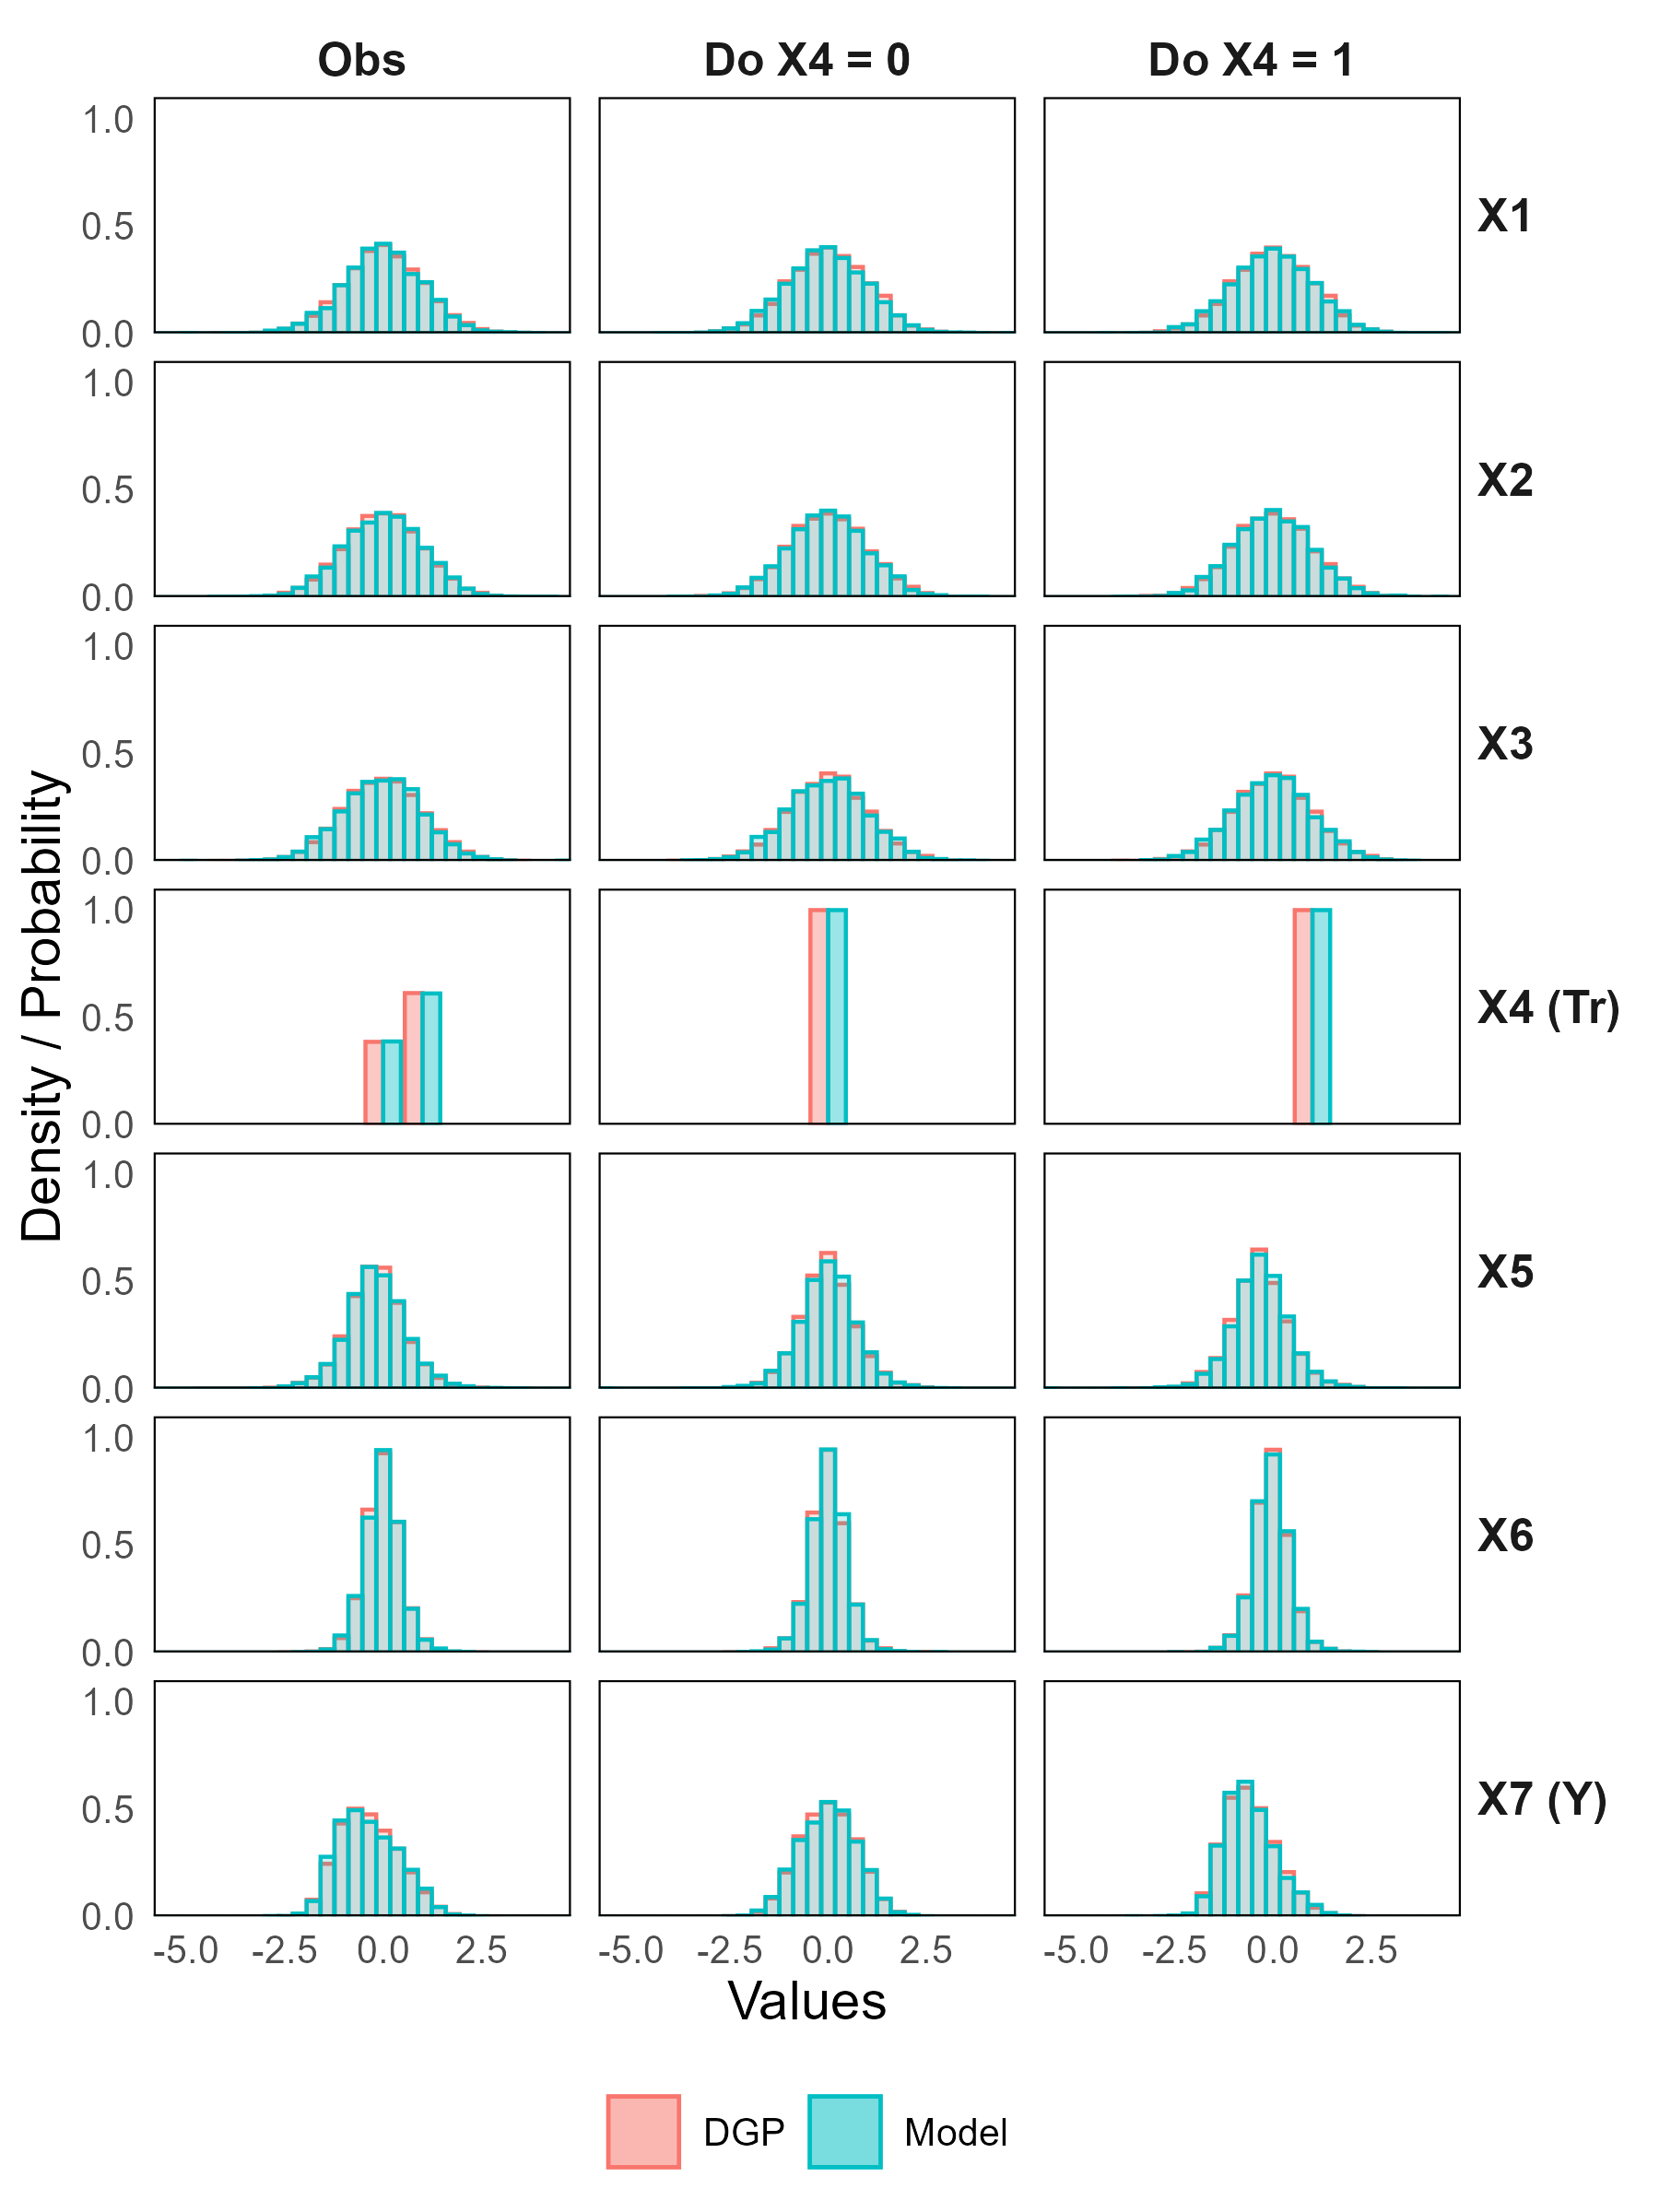
\includegraphics[width=0.45\textwidth]{img/results/observ_scenario2_sampling_distributions_vertical.png}
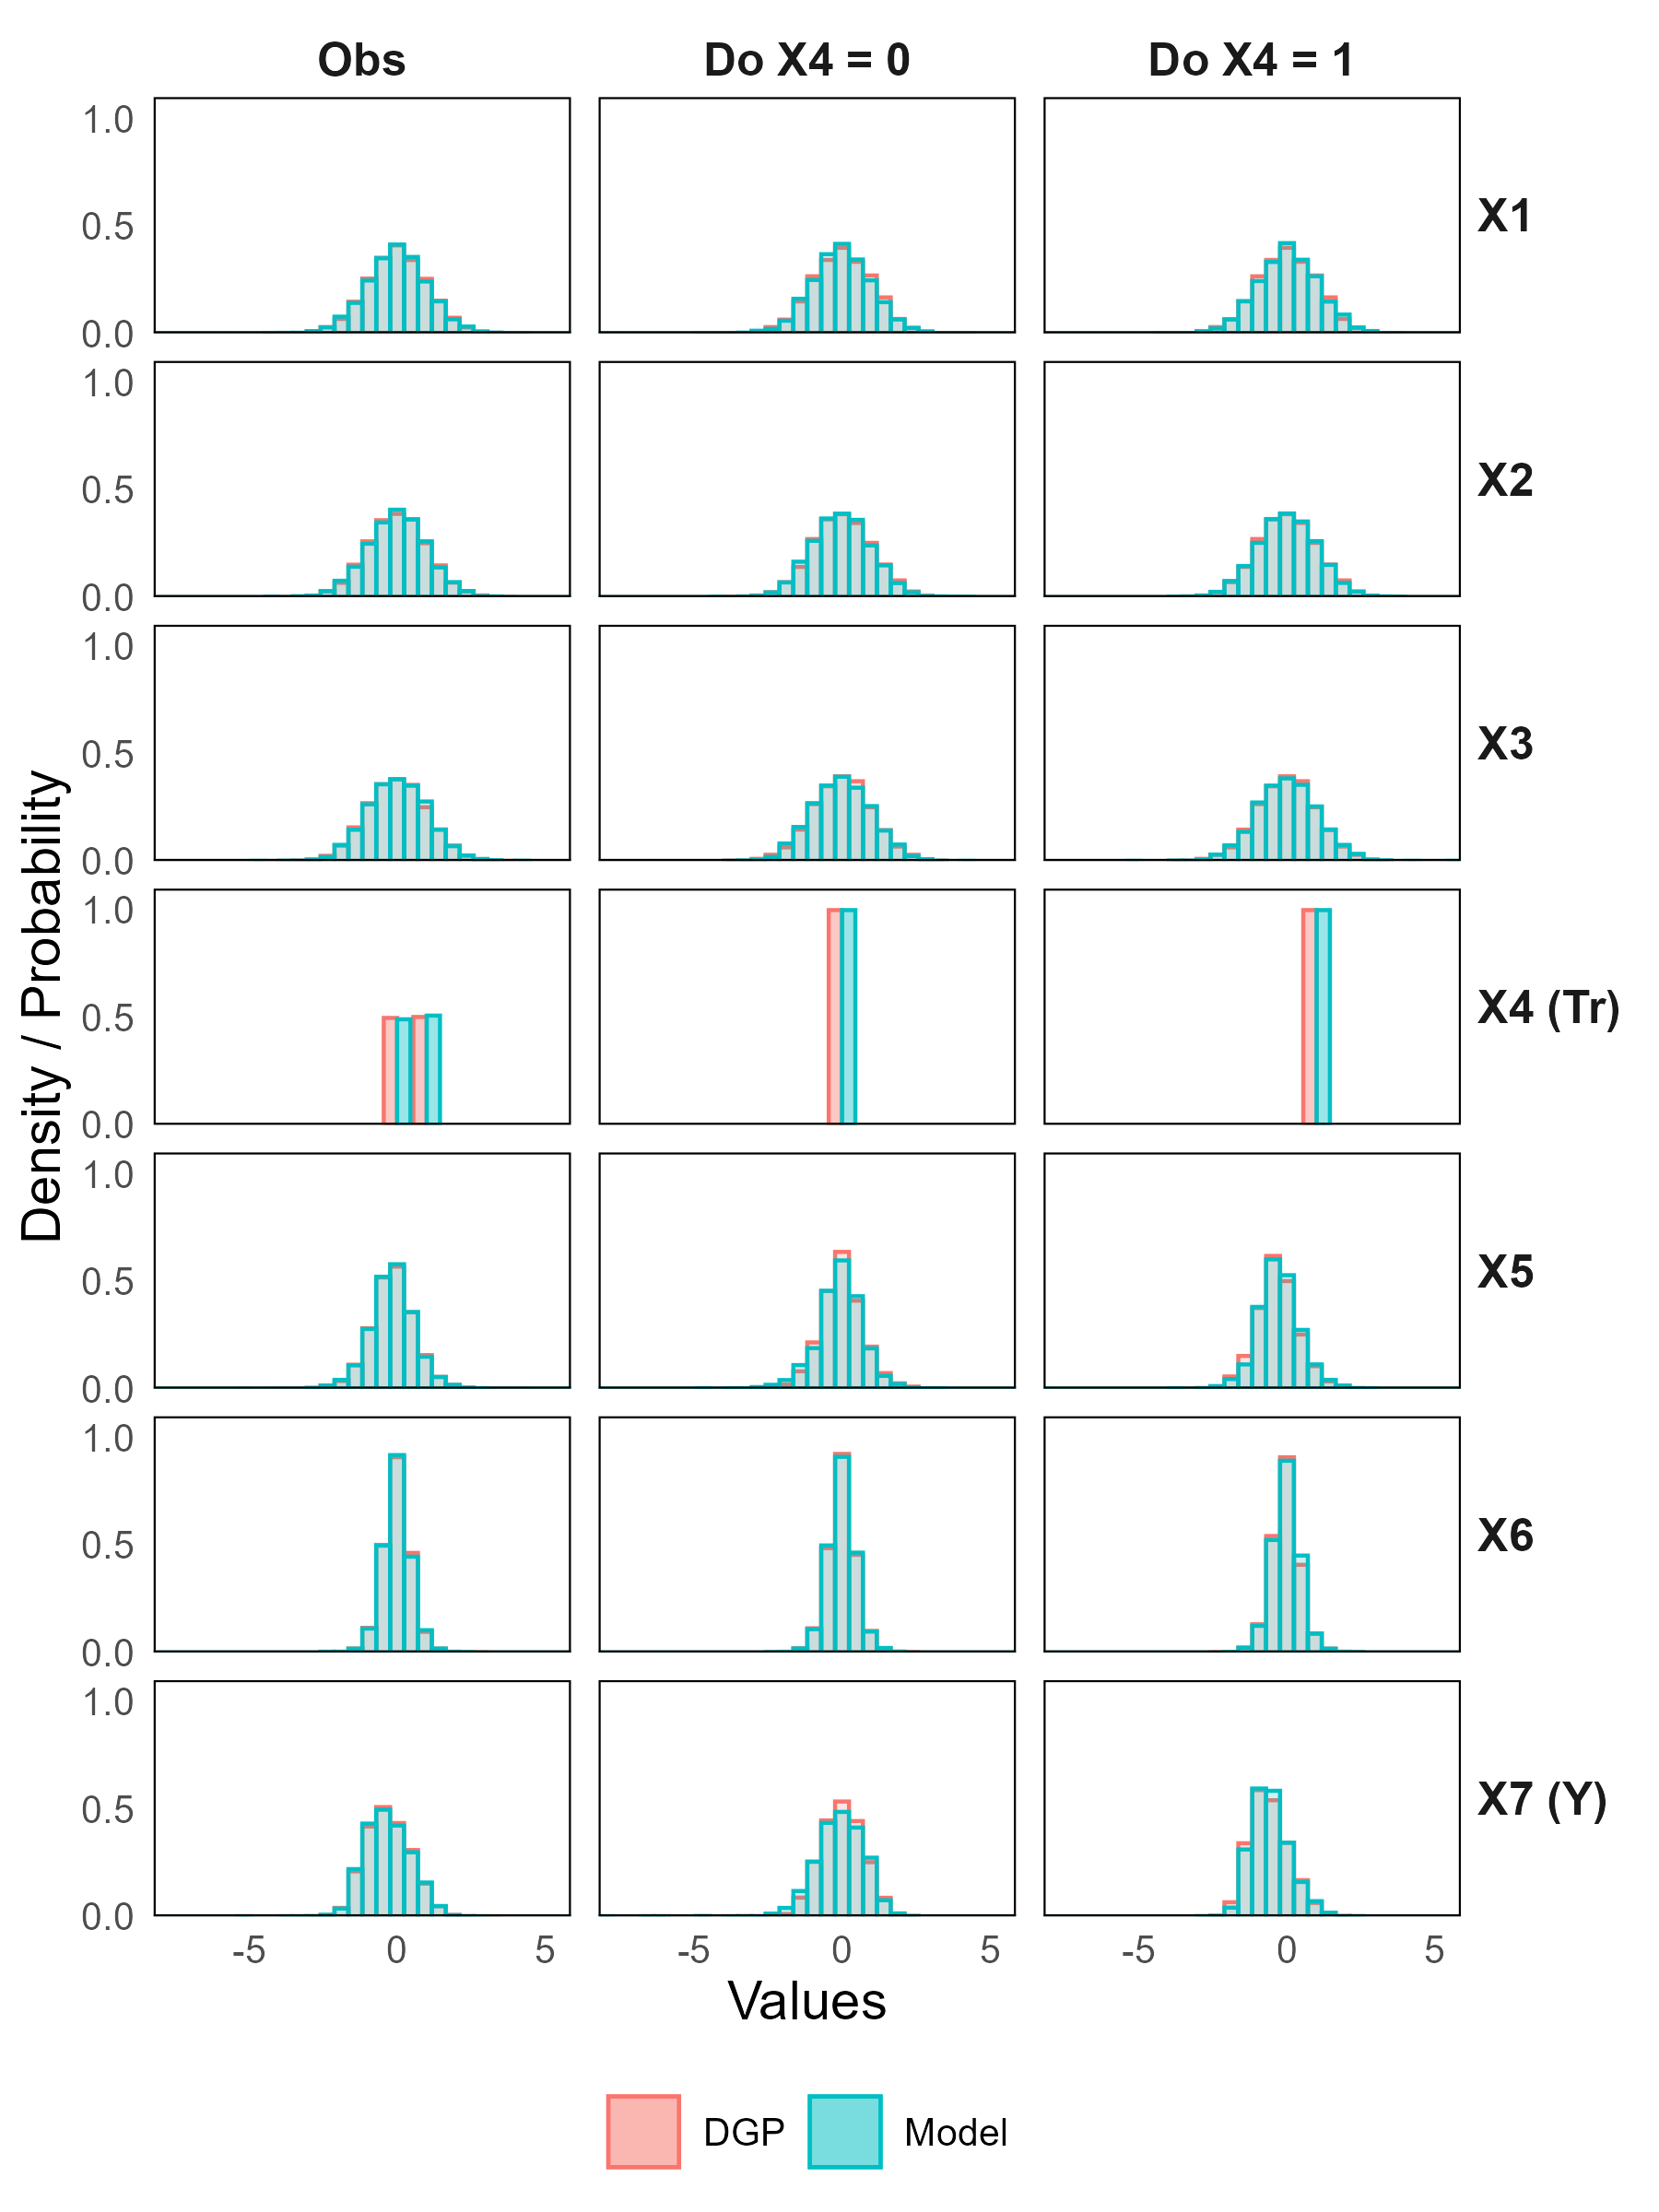
\includegraphics[width=0.45\textwidth]{img/results/rct_scenario2_sampling_distributions_vertical.png}
\caption{Marginal distributions of variables from the DGP and samples generated by the fitted TRAM-DAG for Scenario~(2), which includes a direct treatment effect but no interaction effects. The distributions are shown as observed (Obs), under control intervention (do($X_4 = 0$)), and under treatment intervention (do($X_4 = 1$)). Left: Observational; Right: RCT setting.}
\label{fig:scenario2_sampling_distributions_vertical}
\end{figure}


\begin{figure}[htbp]
\centering
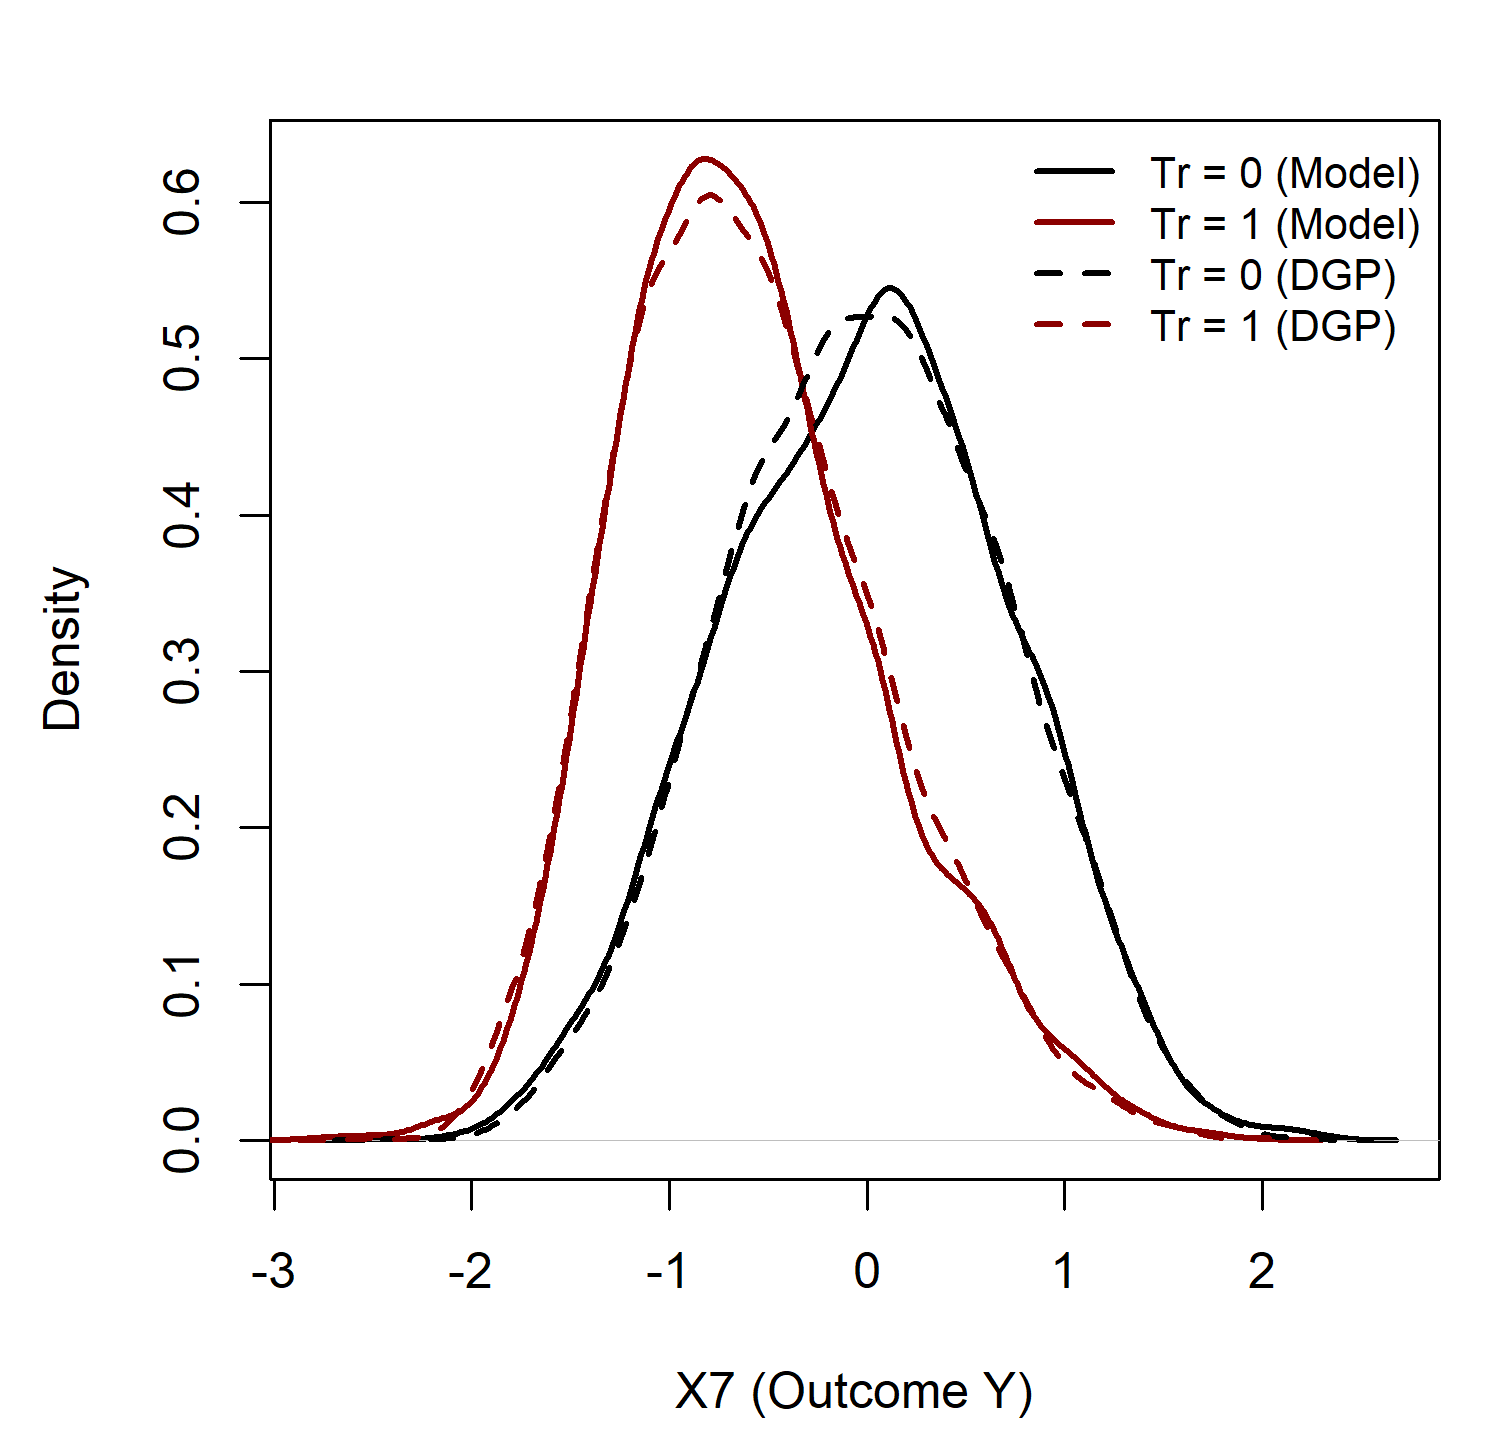
\includegraphics[width=0.45\textwidth]{img/results/observ_scenario2_X7_treatment_densities.png}
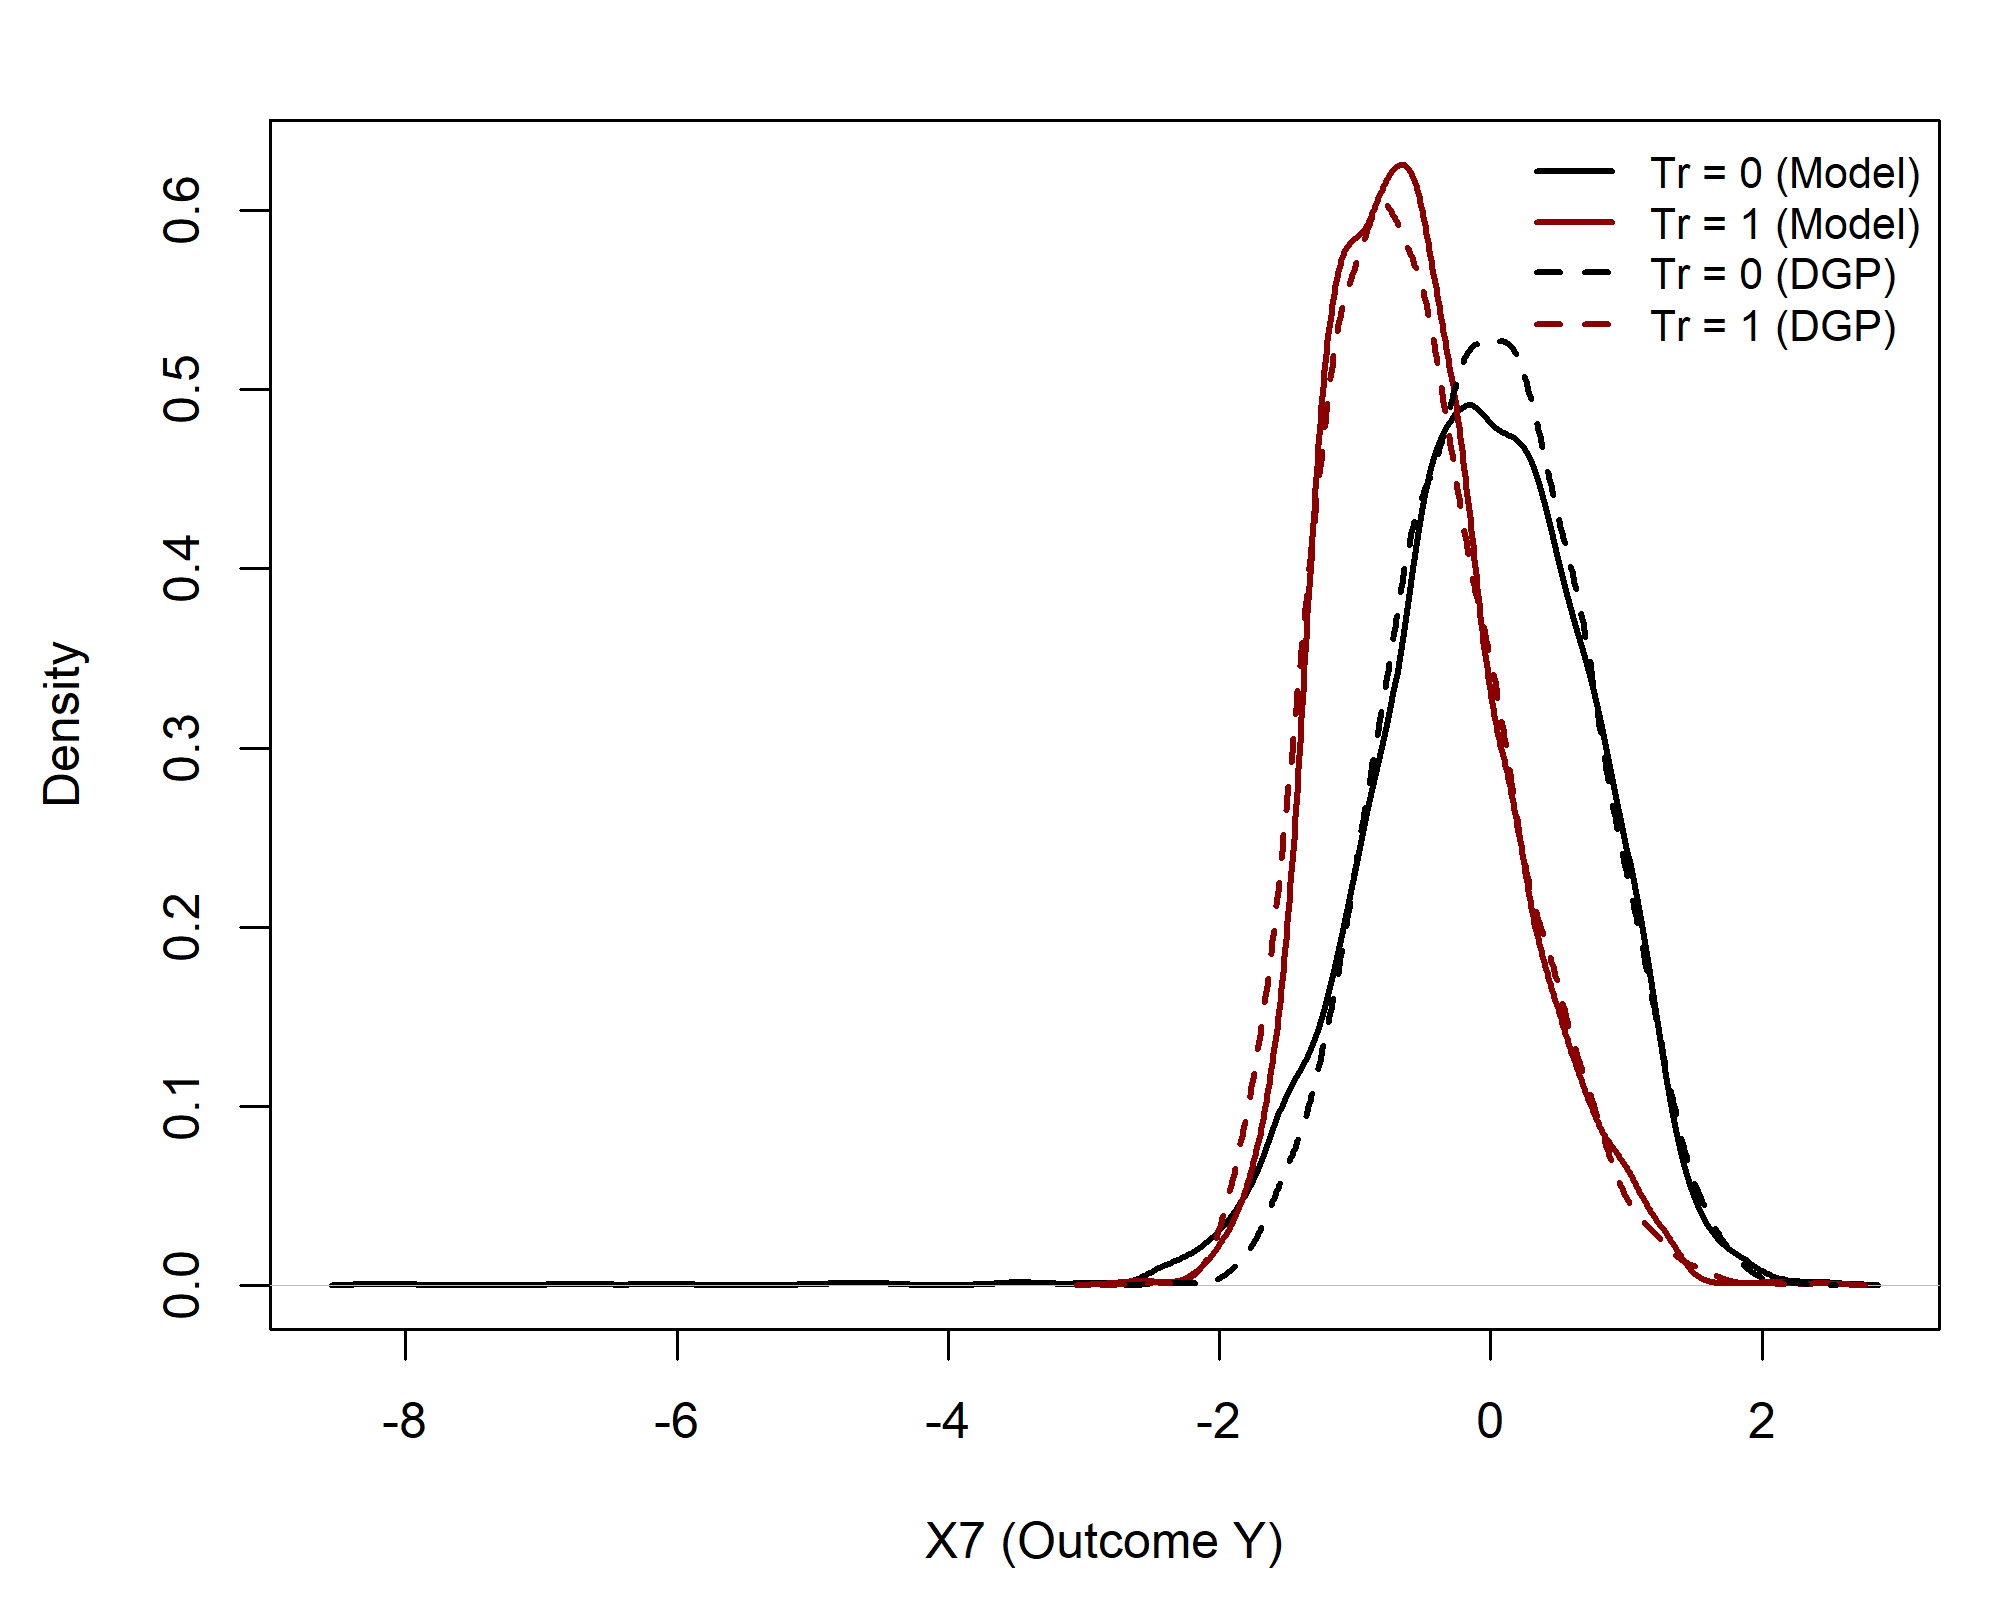
\includegraphics[width=0.45\textwidth]{img/results/rct_scenario2_X7_treatment_densities.png}
\caption{Distributions of the outcome variable ($X_7$) under treatment and control interventions for Scenario~(2), which includes a direct treatment effect but no interaction effects. This plot provides a higher-resolution view of the $X_7$ panels under do($X_4 = 0$) and do($X_4 = 1$) from Figure~\ref{fig:scenario2_sampling_distributions_vertical}. Left: Observational; Right: RCT setting.}
\label{fig:scenario2_outcome_distributions}
\end{figure}






\begin{figure}[htbp]
\centering
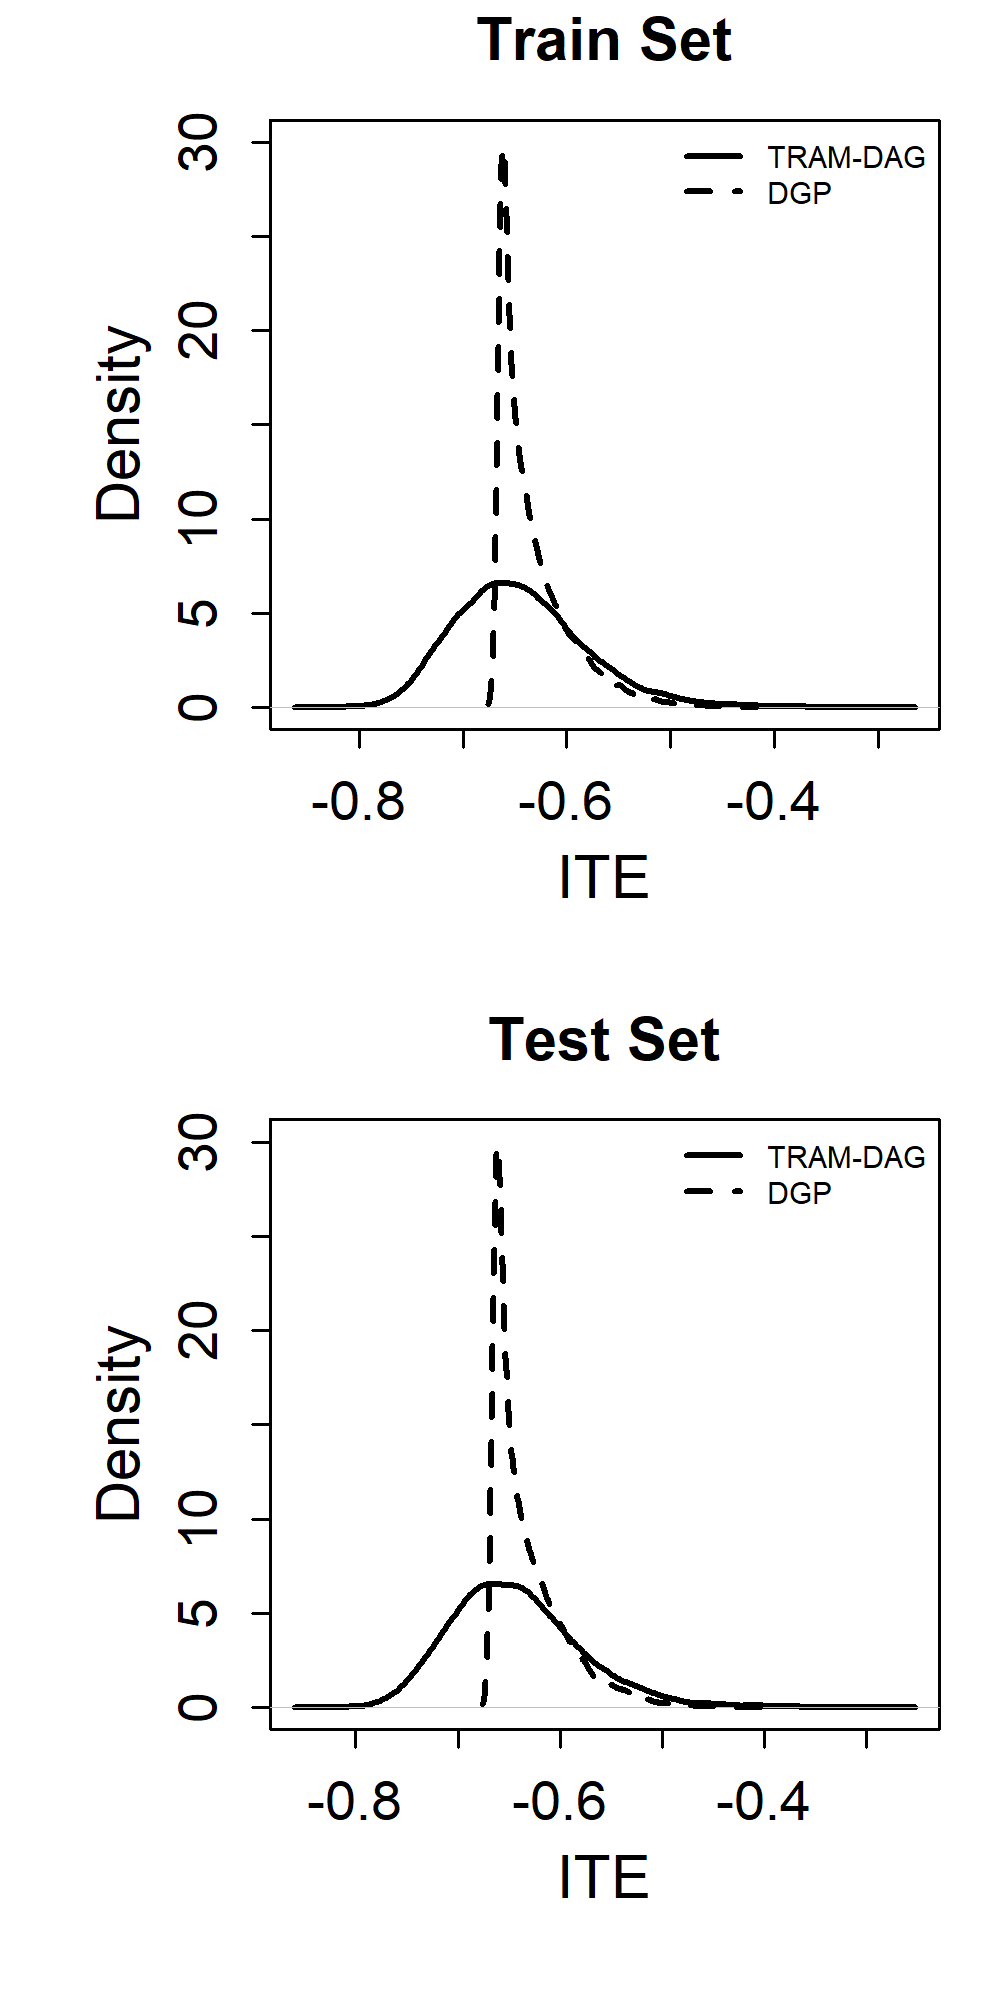
\includegraphics[width=0.33\textwidth]{img/results/observ_scenario2_ITE_densities_train_test.png}
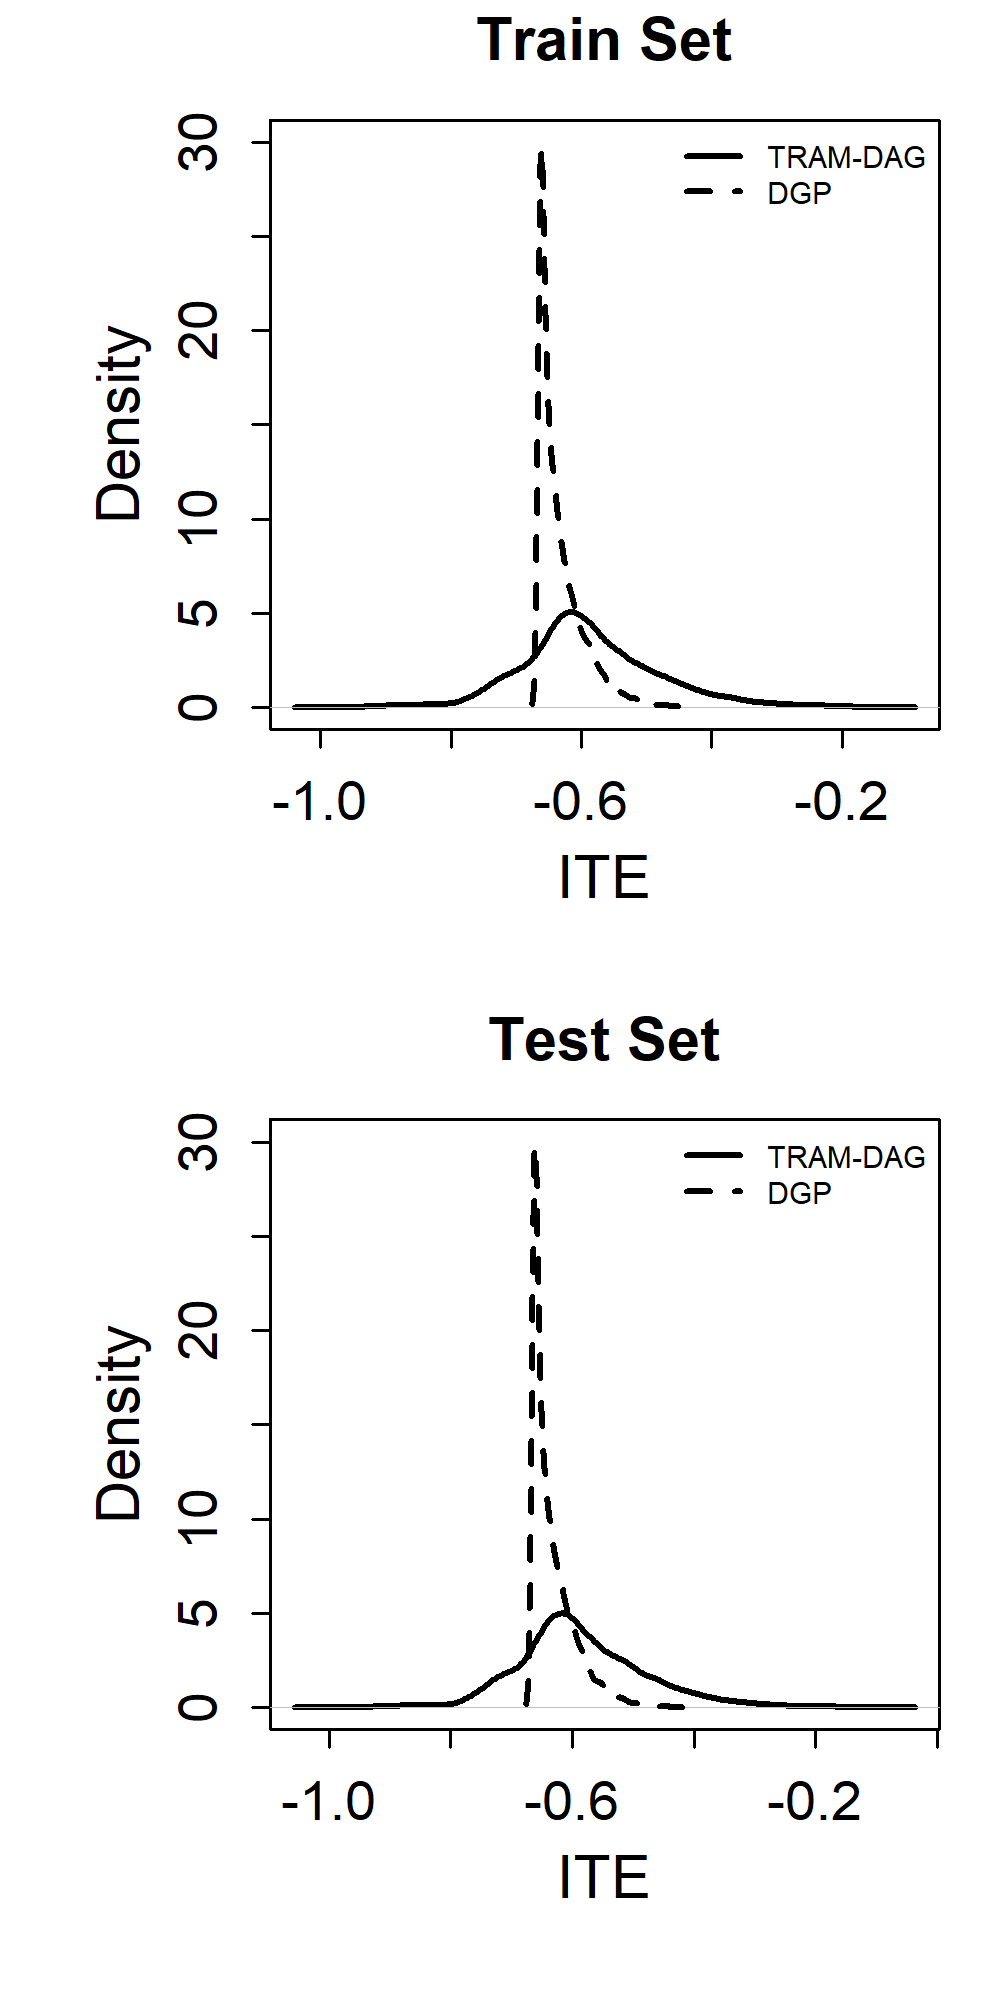
\includegraphics[width=0.33\textwidth]{img/results/rct_scenario2_ITE_densities_train_test.png}
\vspace{-17pt}
\caption{Densities of estimated ITEs compared to the true ITEs in the training and test datasets for Scenario~(2), which includes a direct treatment effect but no interaction effects. Left: Observational; Right: RCT setting.}
\label{fig:scenario2_ite_densities_train_test}
\end{figure}






\begin{figure}[htbp]
\centering
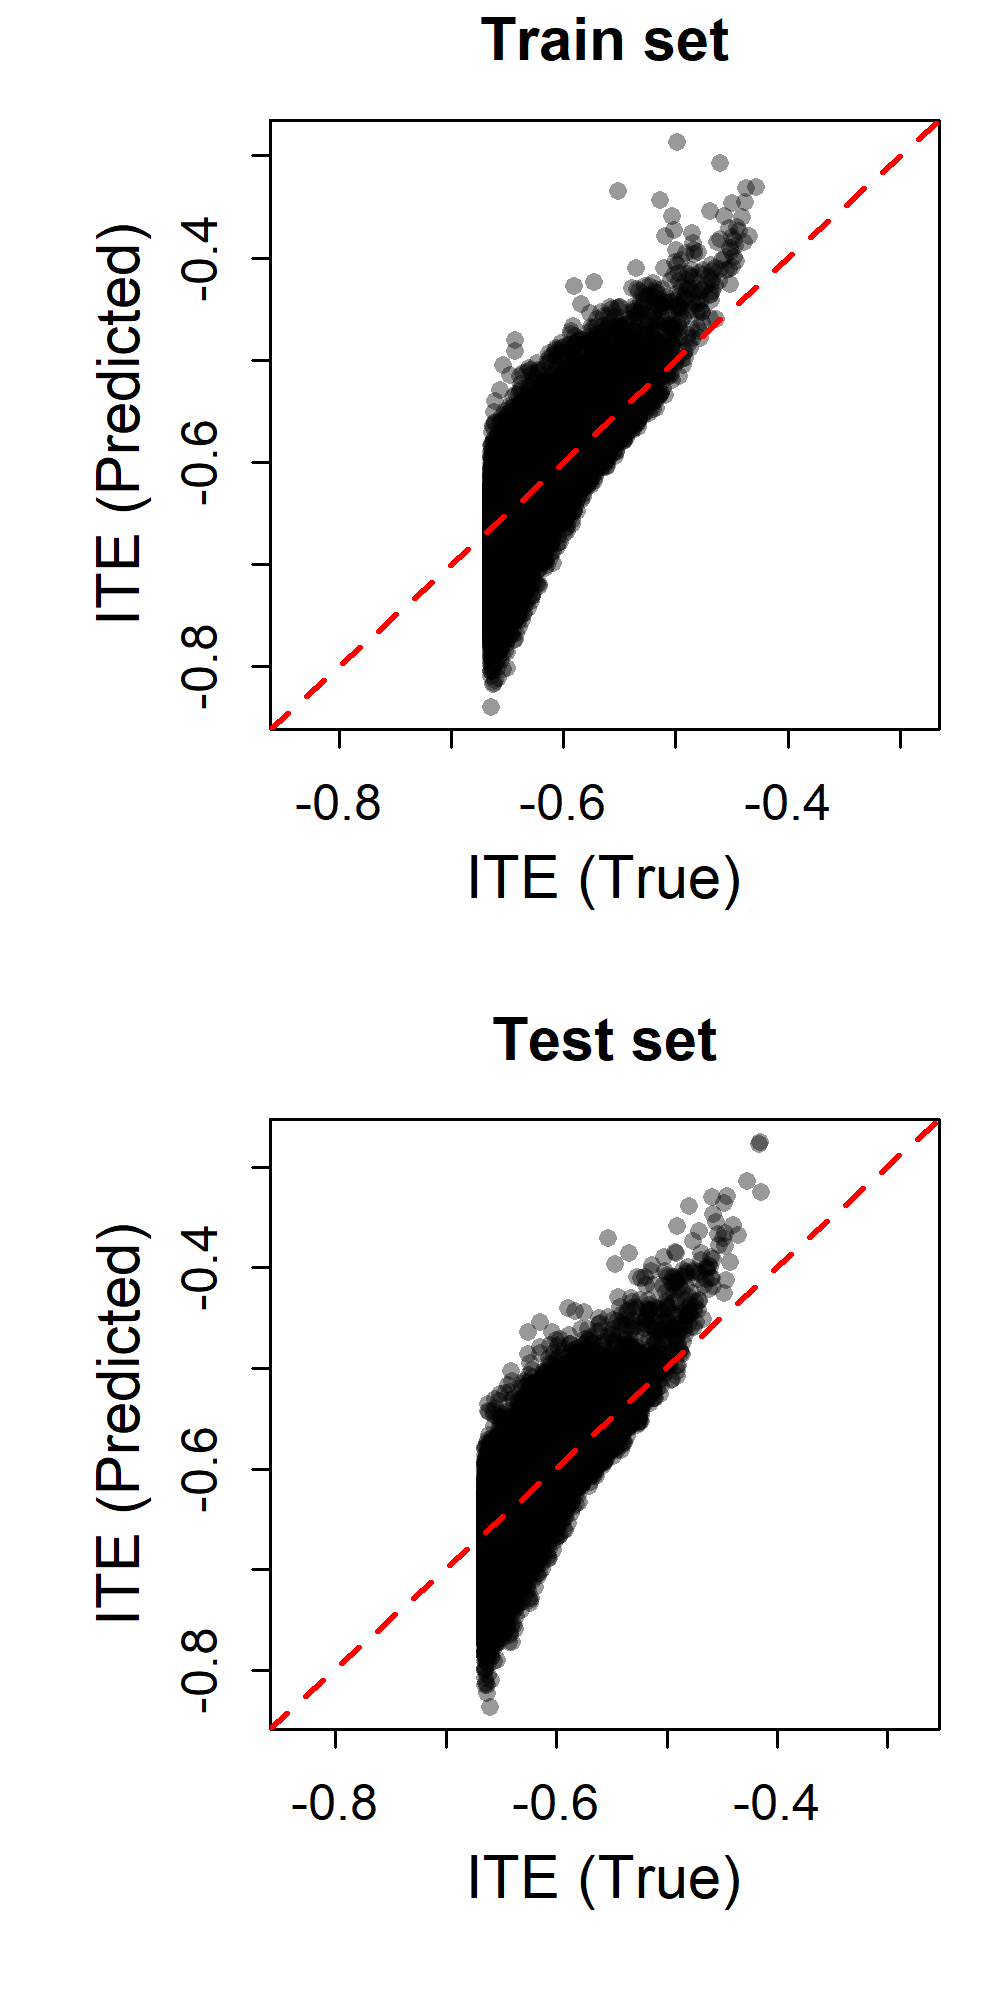
\includegraphics[width=0.33\textwidth]{img/results/observ_scenario2_ITE_scatter_train_test.png}
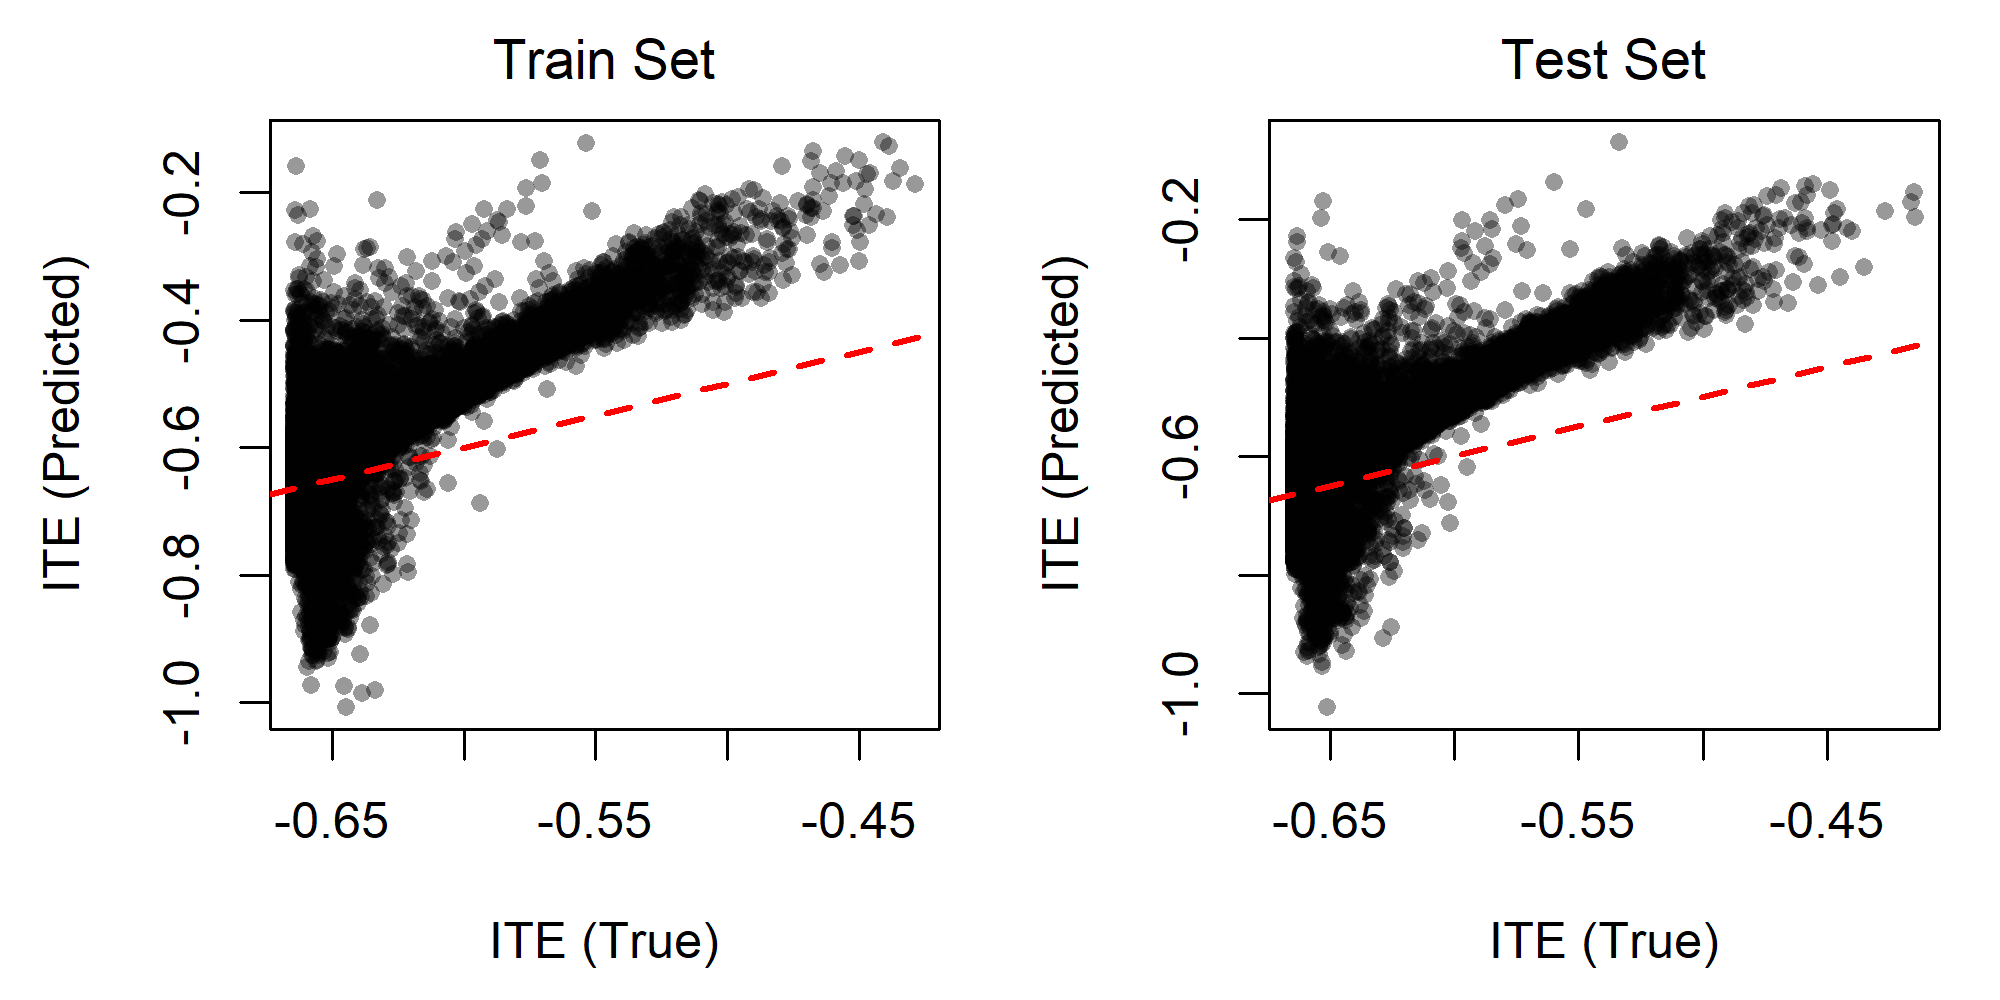
\includegraphics[width=0.33\textwidth]{img/results/rct_scenario2_ITE_scatter_train_test.png}
\vspace{-17pt}
\caption{Scatterplots of estimated ITEs compared to the true ITEs in the training and test datasets for Scenario~(2), which includes a direct treatment effect but no interaction effects. Left: Observational; Right: RCT setting.}
\label{fig:scenario2_ite_scatter_train_test}
\end{figure}




\begin{figure}[htbp]
\centering
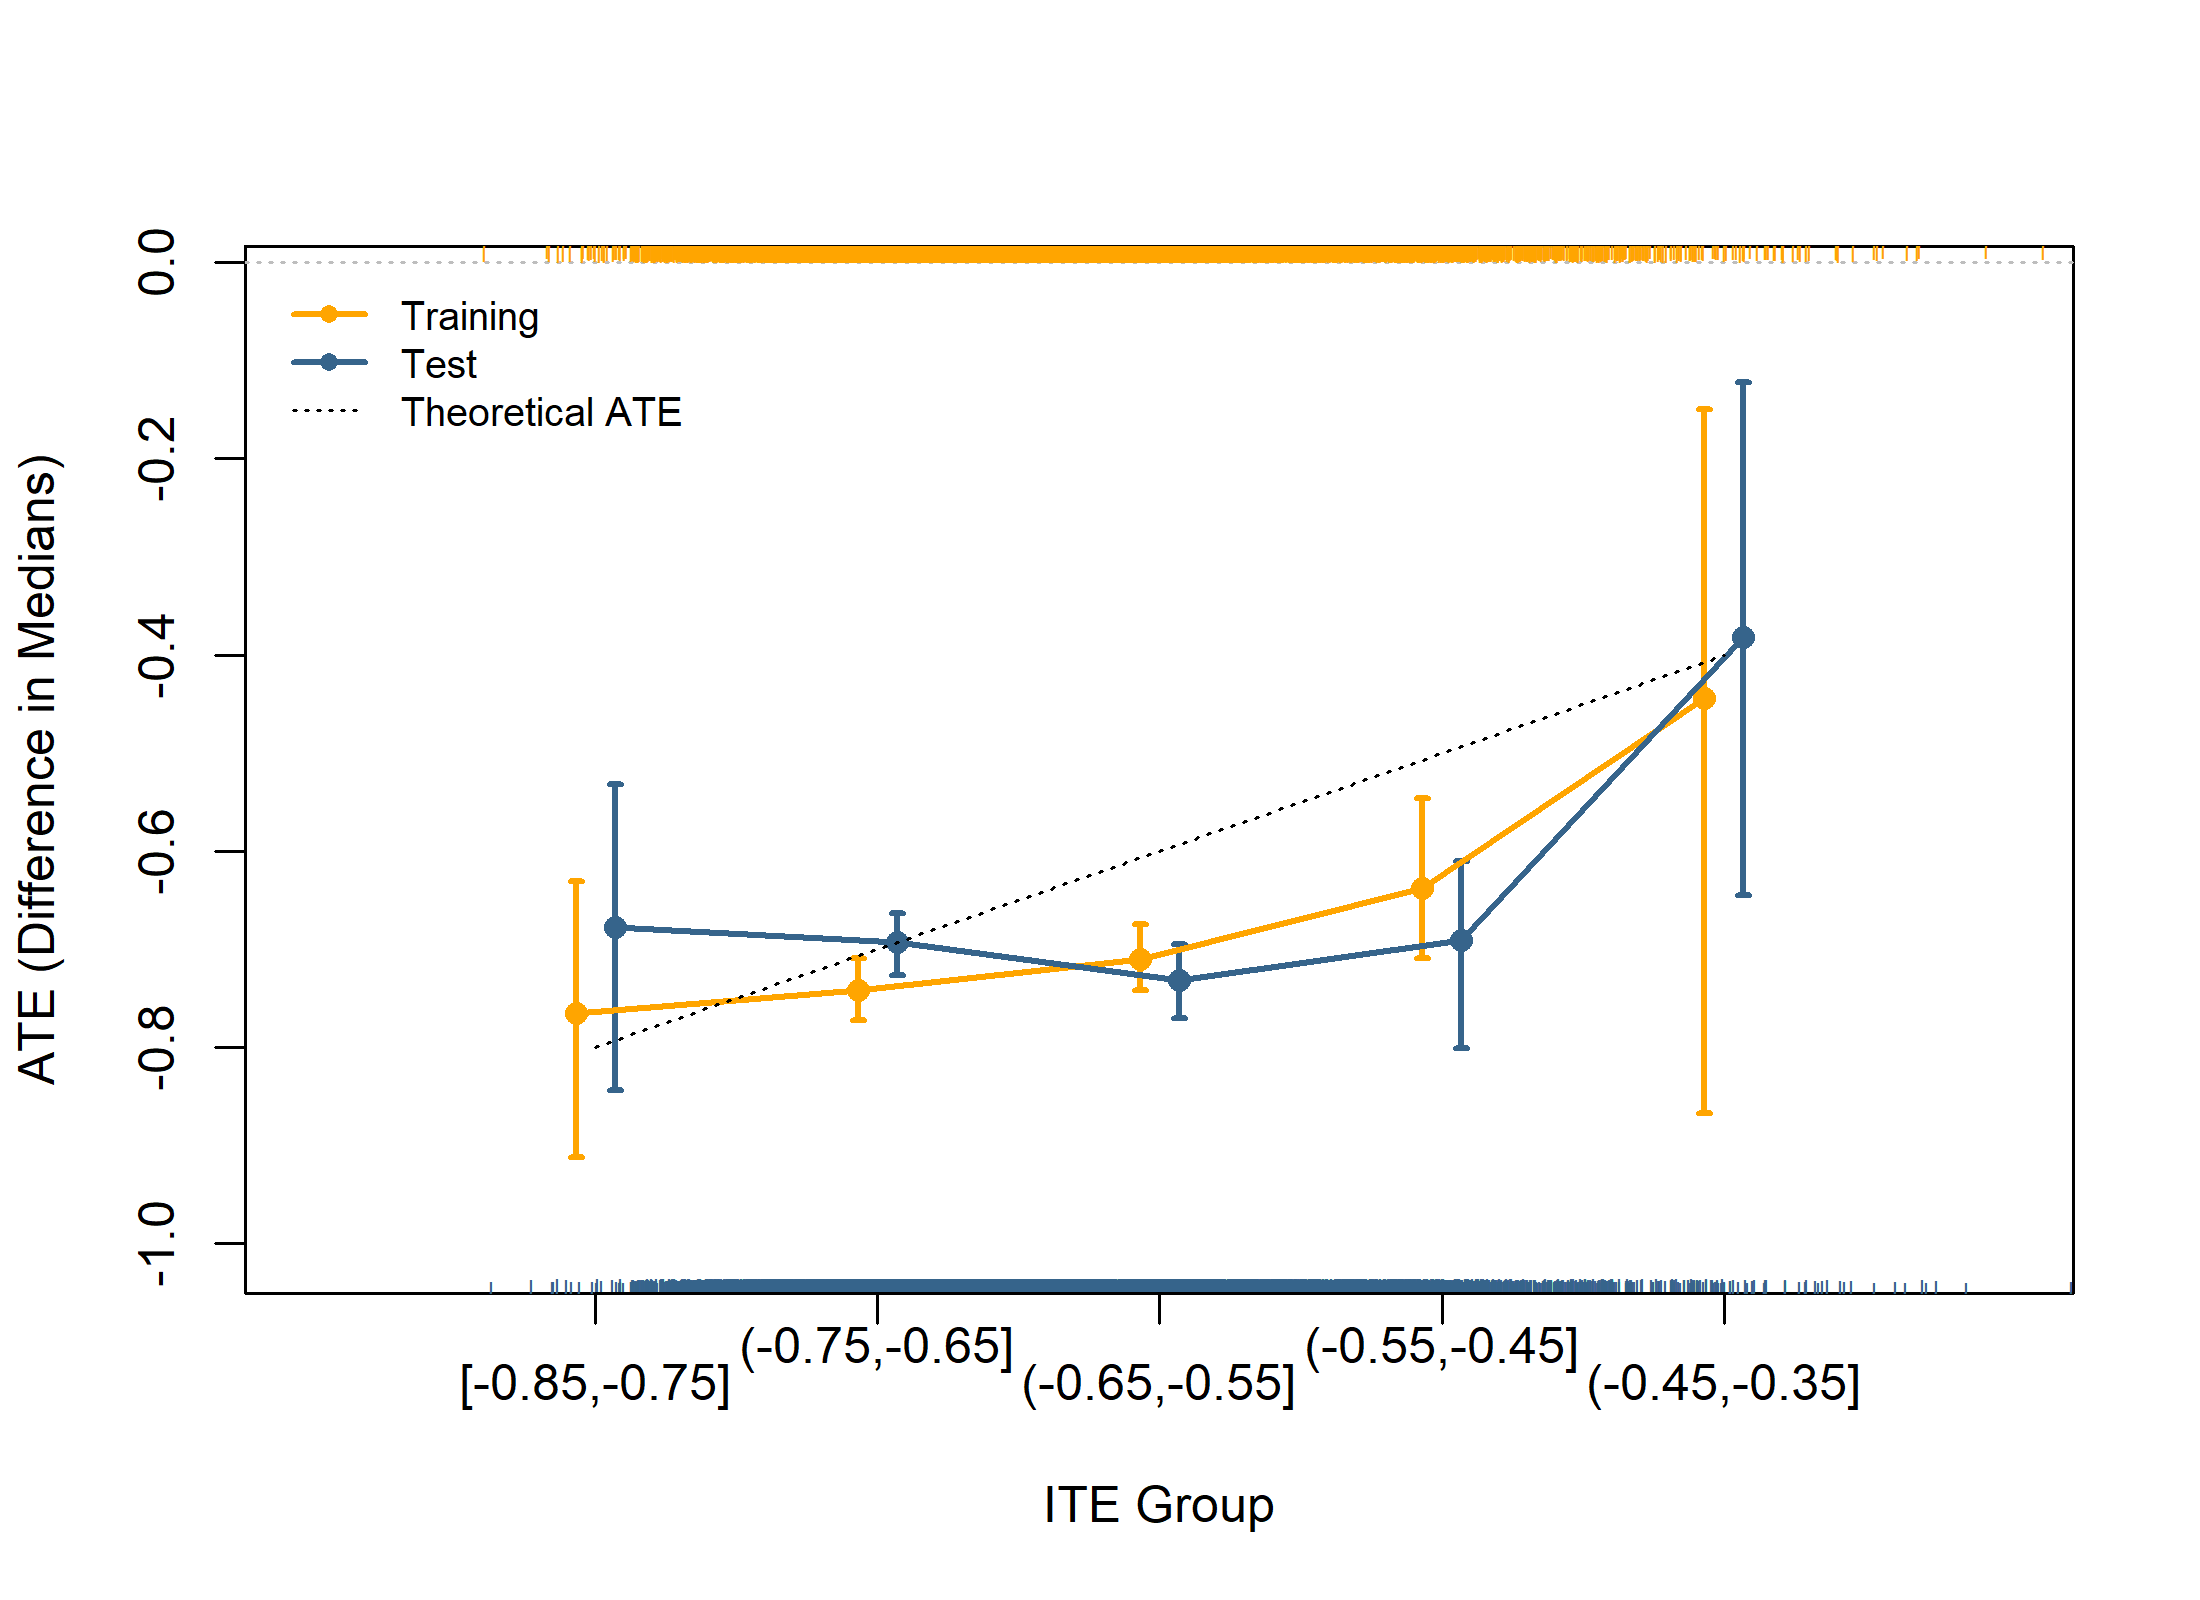
\includegraphics[width=0.8\textwidth]{img/results/observ_scenario2_ITE_ATE.png}
\vspace{-15pt}
\caption{ITE-ATE plot for Scenario~(2) in the observational setting, which includes a direct treatment effect but no interaction effects. Individuals are grouped into bins based on their estimated ITEs, and in each bin, the ATE is computed as the difference in medians of the observed outcomes under treatment and control. The 95\% bootstrap confidence intervals indicate uncertainty.}
\label{fig:observ_scenario2_ite_ATE}
\end{figure}



\begin{figure}[htbp]
\centering
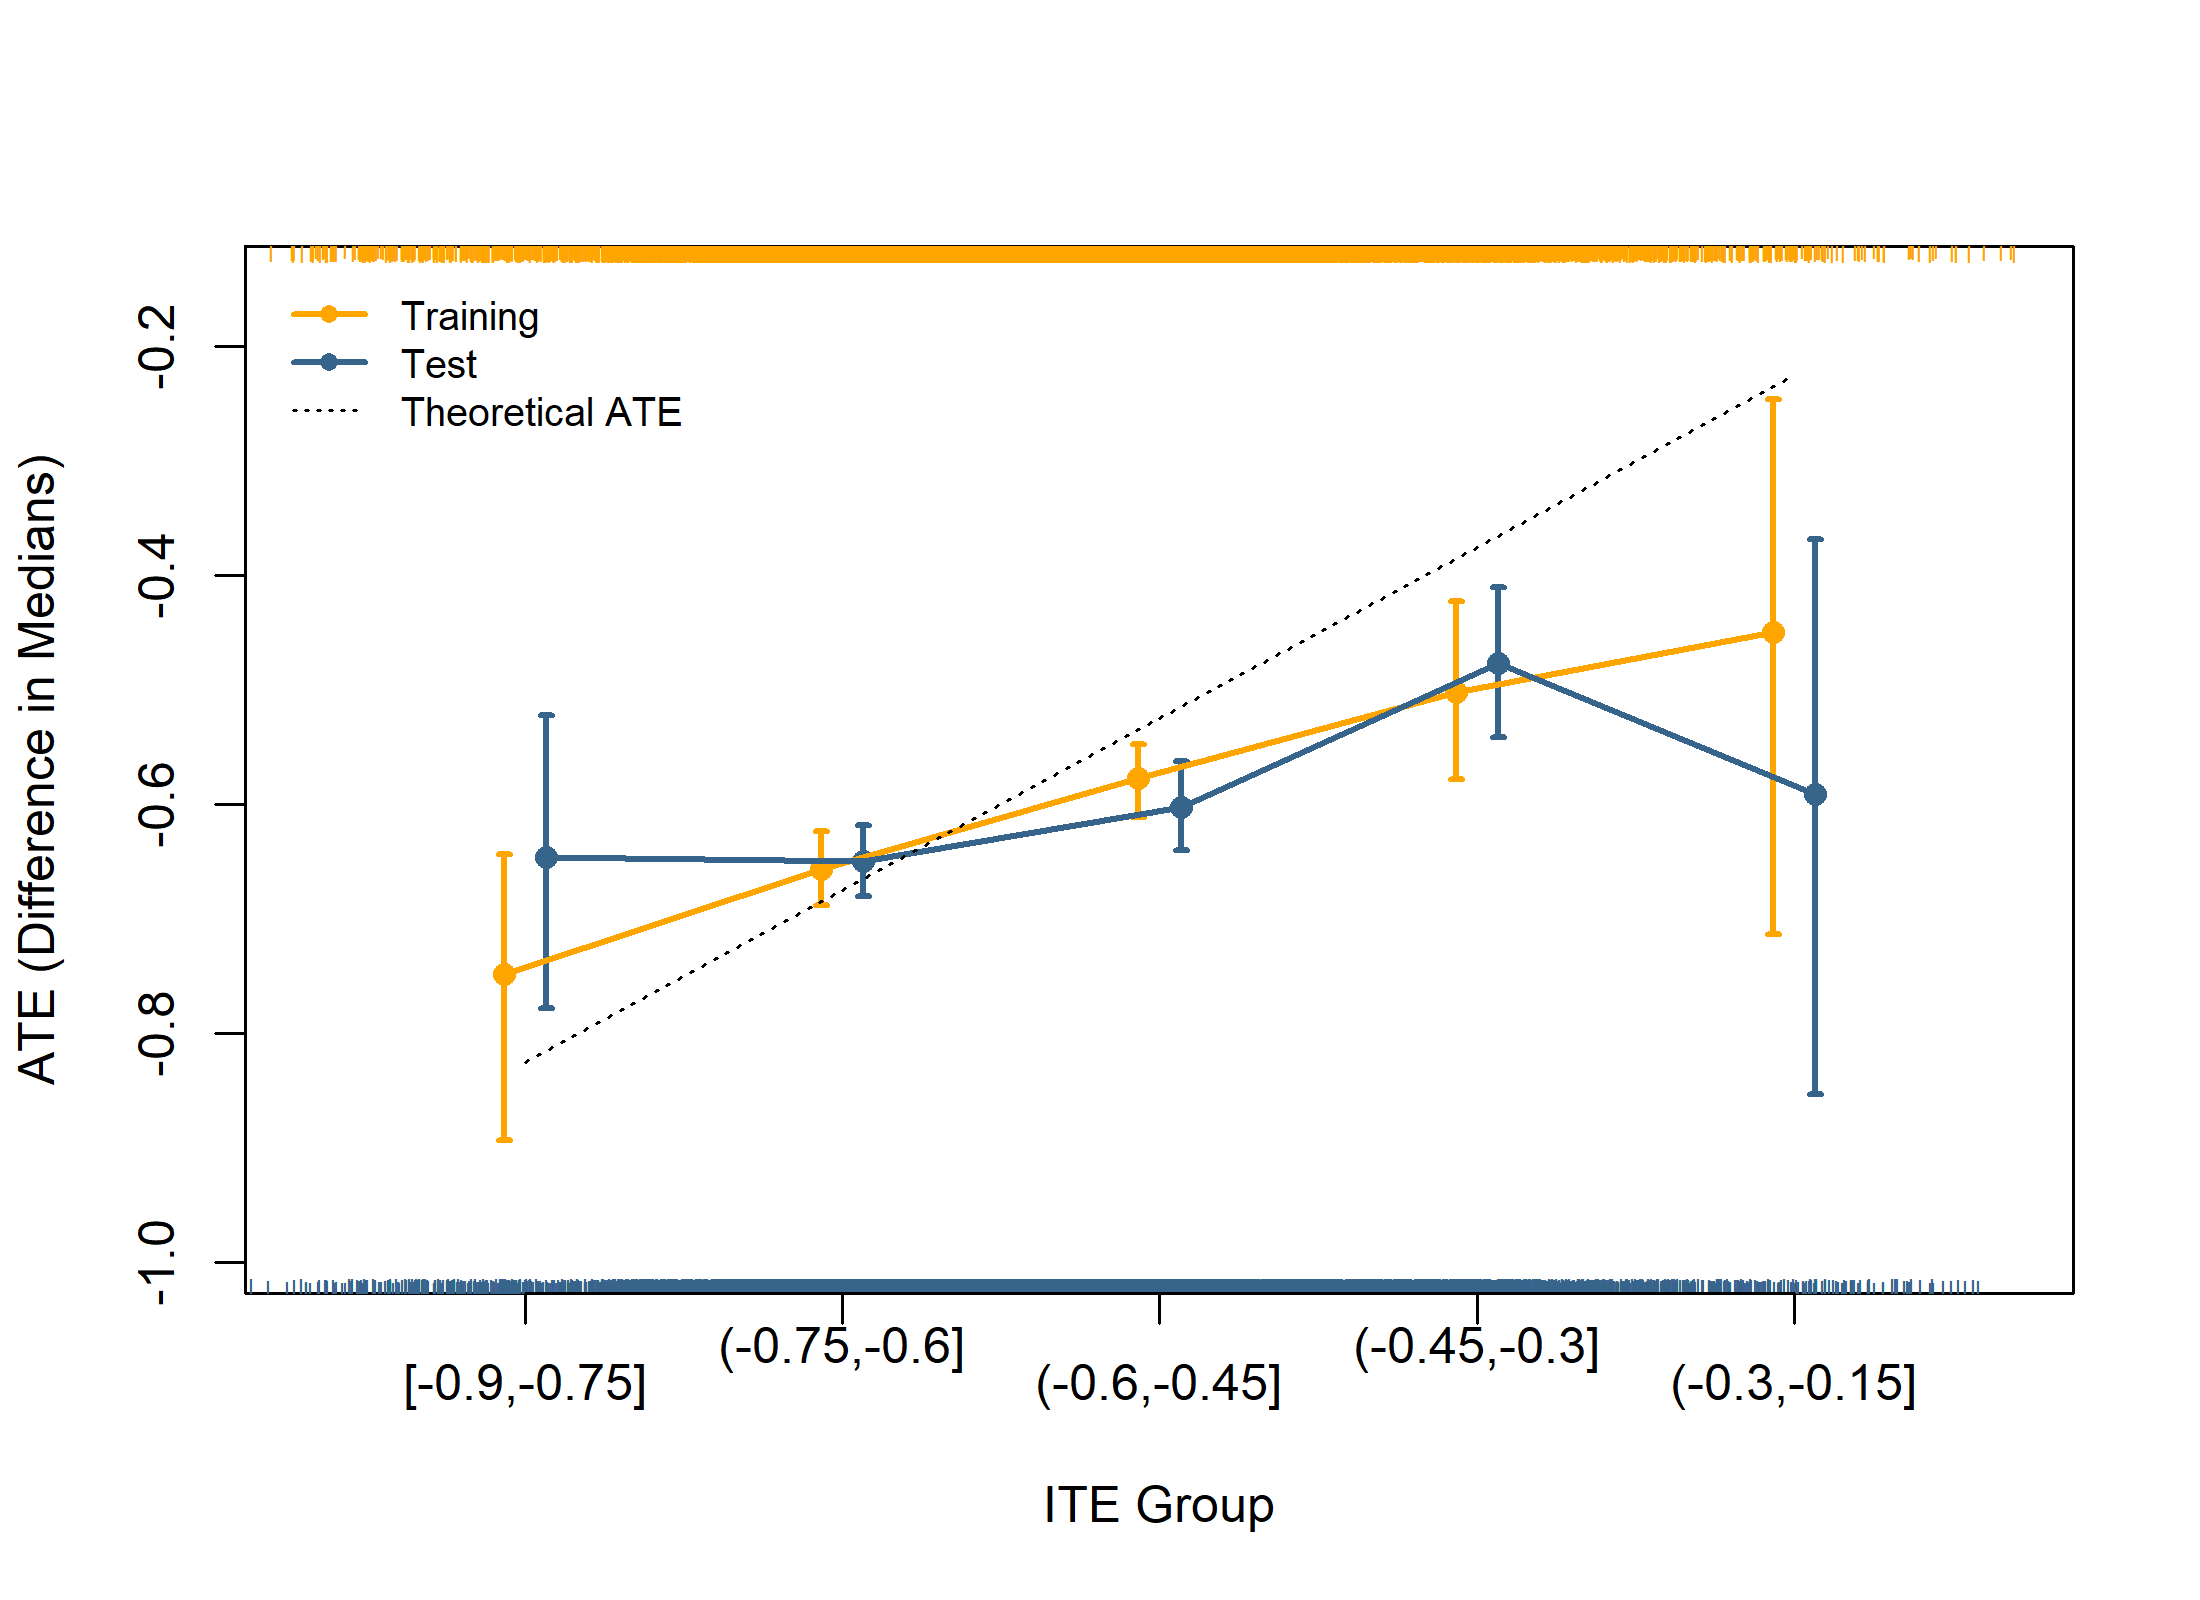
\includegraphics[width=0.8\textwidth]{img/results/rct_scenario2_ITE_ATE.png}
\vspace{-15pt}
\caption{ITE-ATE plot for Scenario~(2) in the RCT setting, which includes a direct treatment effect but no interaction effects. Individuals are grouped into bins based on their estimated ITEs, and in each bin, the ATE is computed as the difference in medians of the observed outcomes under treatment and control. The 95\% bootstrap confidence intervals indicate uncertainty.}
\label{fig:rct_scenario2_ite_ATE}
\end{figure}



\clearpage 



\subsection{Scenario (3): No direct effect, but with interaction effects}

\begin{figure}[H]
\centering
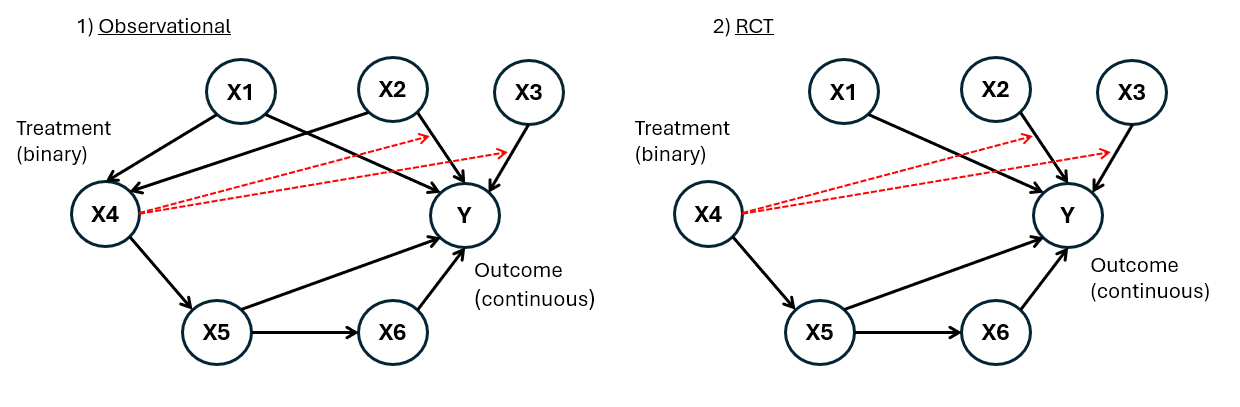
\includegraphics[width=0.85\textwidth]{img/exp4_dag_3.png}
\caption{DAGs for Scenario~(3), which includes no direct effect of the treatment on the outcome, but interaction effects with covariates $X_2$ and $X_3$. Left: Observational setting; Right: RCT setting.}
\label{fig:ite_dag_observational_3}
\end{figure}

Scenario~(3) includes no direct effect of the treatment on the outcome, but does include interaction effects between the treatment and covariates $X_2$ and $X_3$. Compared to Scenario~(1), removing the direct effect results in a more centered ITE distribution, as shown in Figure~\ref{fig:scenario3_ite_distribution_dgp}. In the test set of the RCT setting, the ATE measured as the difference in means was -0.048, with a 95\% confidence interval from -0.068 to -0.028.




\begin{table}[htbp]
\centering
\small
\caption{Scenario (3), without a direct treatment effect but including interaction effects: Comparison of ATE measures across train and test sets for the observational and RCT setting. $\text{Y}_\text{observed}^{(\text{Tr})}$ denotes the observed outcome under the treatment ($\text{Tr}$) actually received. The estimated ATE from $\text{mean}(\text{ITE}_\text{estimated})$ can be directly compared to the true $\text{mean}(\text{ITE}_\text{true})$, whereas comparisons to the empirical ATEs based on outcome differences should be interpreted with caution.}
\label{tab:scenario3_ate_comparison}
\begin{tabular}{l c c c c}
\toprule
\textbf{Measure} & \multicolumn{2}{c}{\textbf{Observational}} & \multicolumn{2}{c}{\textbf{RCT}} \\
\cmidrule(lr){2-3} \cmidrule(lr){4-5}
 & \textbf{Train} & \textbf{Test} & \textbf{Train} & \textbf{Test} \\
\midrule
ATE as $\text{mean}(\text{Y}_\text{observed}^{(1)}) - \text{mean}(\text{Y}_\text{observed}^{(0)})$ 
& NA & NA 
& -0.048 
& -0.048 \\

ATE as $\text{median}(\text{Y}_\text{observed}^{(1)}) - \text{median}(\text{Y}_\text{observed}^{(0)})$  
& NA & NA 
& -0.048 
& -0.059 \\

ATE as mean(ITE$_\text{true}$)  
& -0.065 
& -0.068 
& -0.065 
& -0.068 \\

ATE as mean(ITE$_\text{estimated}$) 
& -0.059 
& -0.061 
& -0.051 
& -0.053 \\
\bottomrule
\end{tabular}
\end{table}


% \begin{table}[htbp]
% \centering
% \small
% \caption{Scenario (3), without direct treatment effect but including interaction effects: Comparison of ATE measures across train and test sets for the observational and RCT setting.}
% \label{tab:scenario3_ate_comparison_old}
% \begin{tabular}{l c c c c}
% \toprule
% \textbf{Measure} & \multicolumn{2}{c}{\textbf{Observational}} & \multicolumn{2}{c}{\textbf{RCT}} \\
% \cmidrule(lr){2-3} \cmidrule(lr){4-5}
%  & \textbf{Train} & \textbf{Test} & \textbf{Train} & \textbf{Test} \\
% \midrule
% ATE as $\text{mean}(\text{Y}_\text{observed}^{(1)}) - \text{mean}(\text{Y}_\text{observed}^{(0)})$ & NA & NA & round(rct_scenario3$dev_ATE_observed_Y_mean_diff, 3) & round(rct_scenario3$val_ATE_observed_Y_mean_diff, 3) \\
% ATE as $\text{median}(\text{Y}_\text{observed}^{(1)}) - \text{median}(\text{Y}_\text{observed}^{(0)})$ & NA & NA & round(rct_scenario3$dev_ATE_observed_Y_median_diff, 3) & round(rct_scenario3$val_ATE_observed_Y_median_diff, 3) \\
% ATE as mean(ITE$_\text{true}$)  & round(observ_scenario3$dev_ITE_median_average, 3) & round(observ_scenario3$val_ITE_median_average, 3) & round(rct_scenario3$dev_ITE_median_average, 3) & round(rct_scenario3$val_ITE_median_average, 3) \\
% ATE as mean(ITE$_\text{estimated}$) & round(observ_scenario3$dev_ITE_median_pred_average, 3) & round(observ_scenario3$val_ITE_median_pred_average, 3) & round(rct_scenario3$dev_ITE_median_pred_average, 3) & round(rct_scenario3$val_ITE_median_pred_average, 3) \\
% \bottomrule
% \end{tabular}
% \end{table}
% 


\begin{figure}[htbp]
\centering
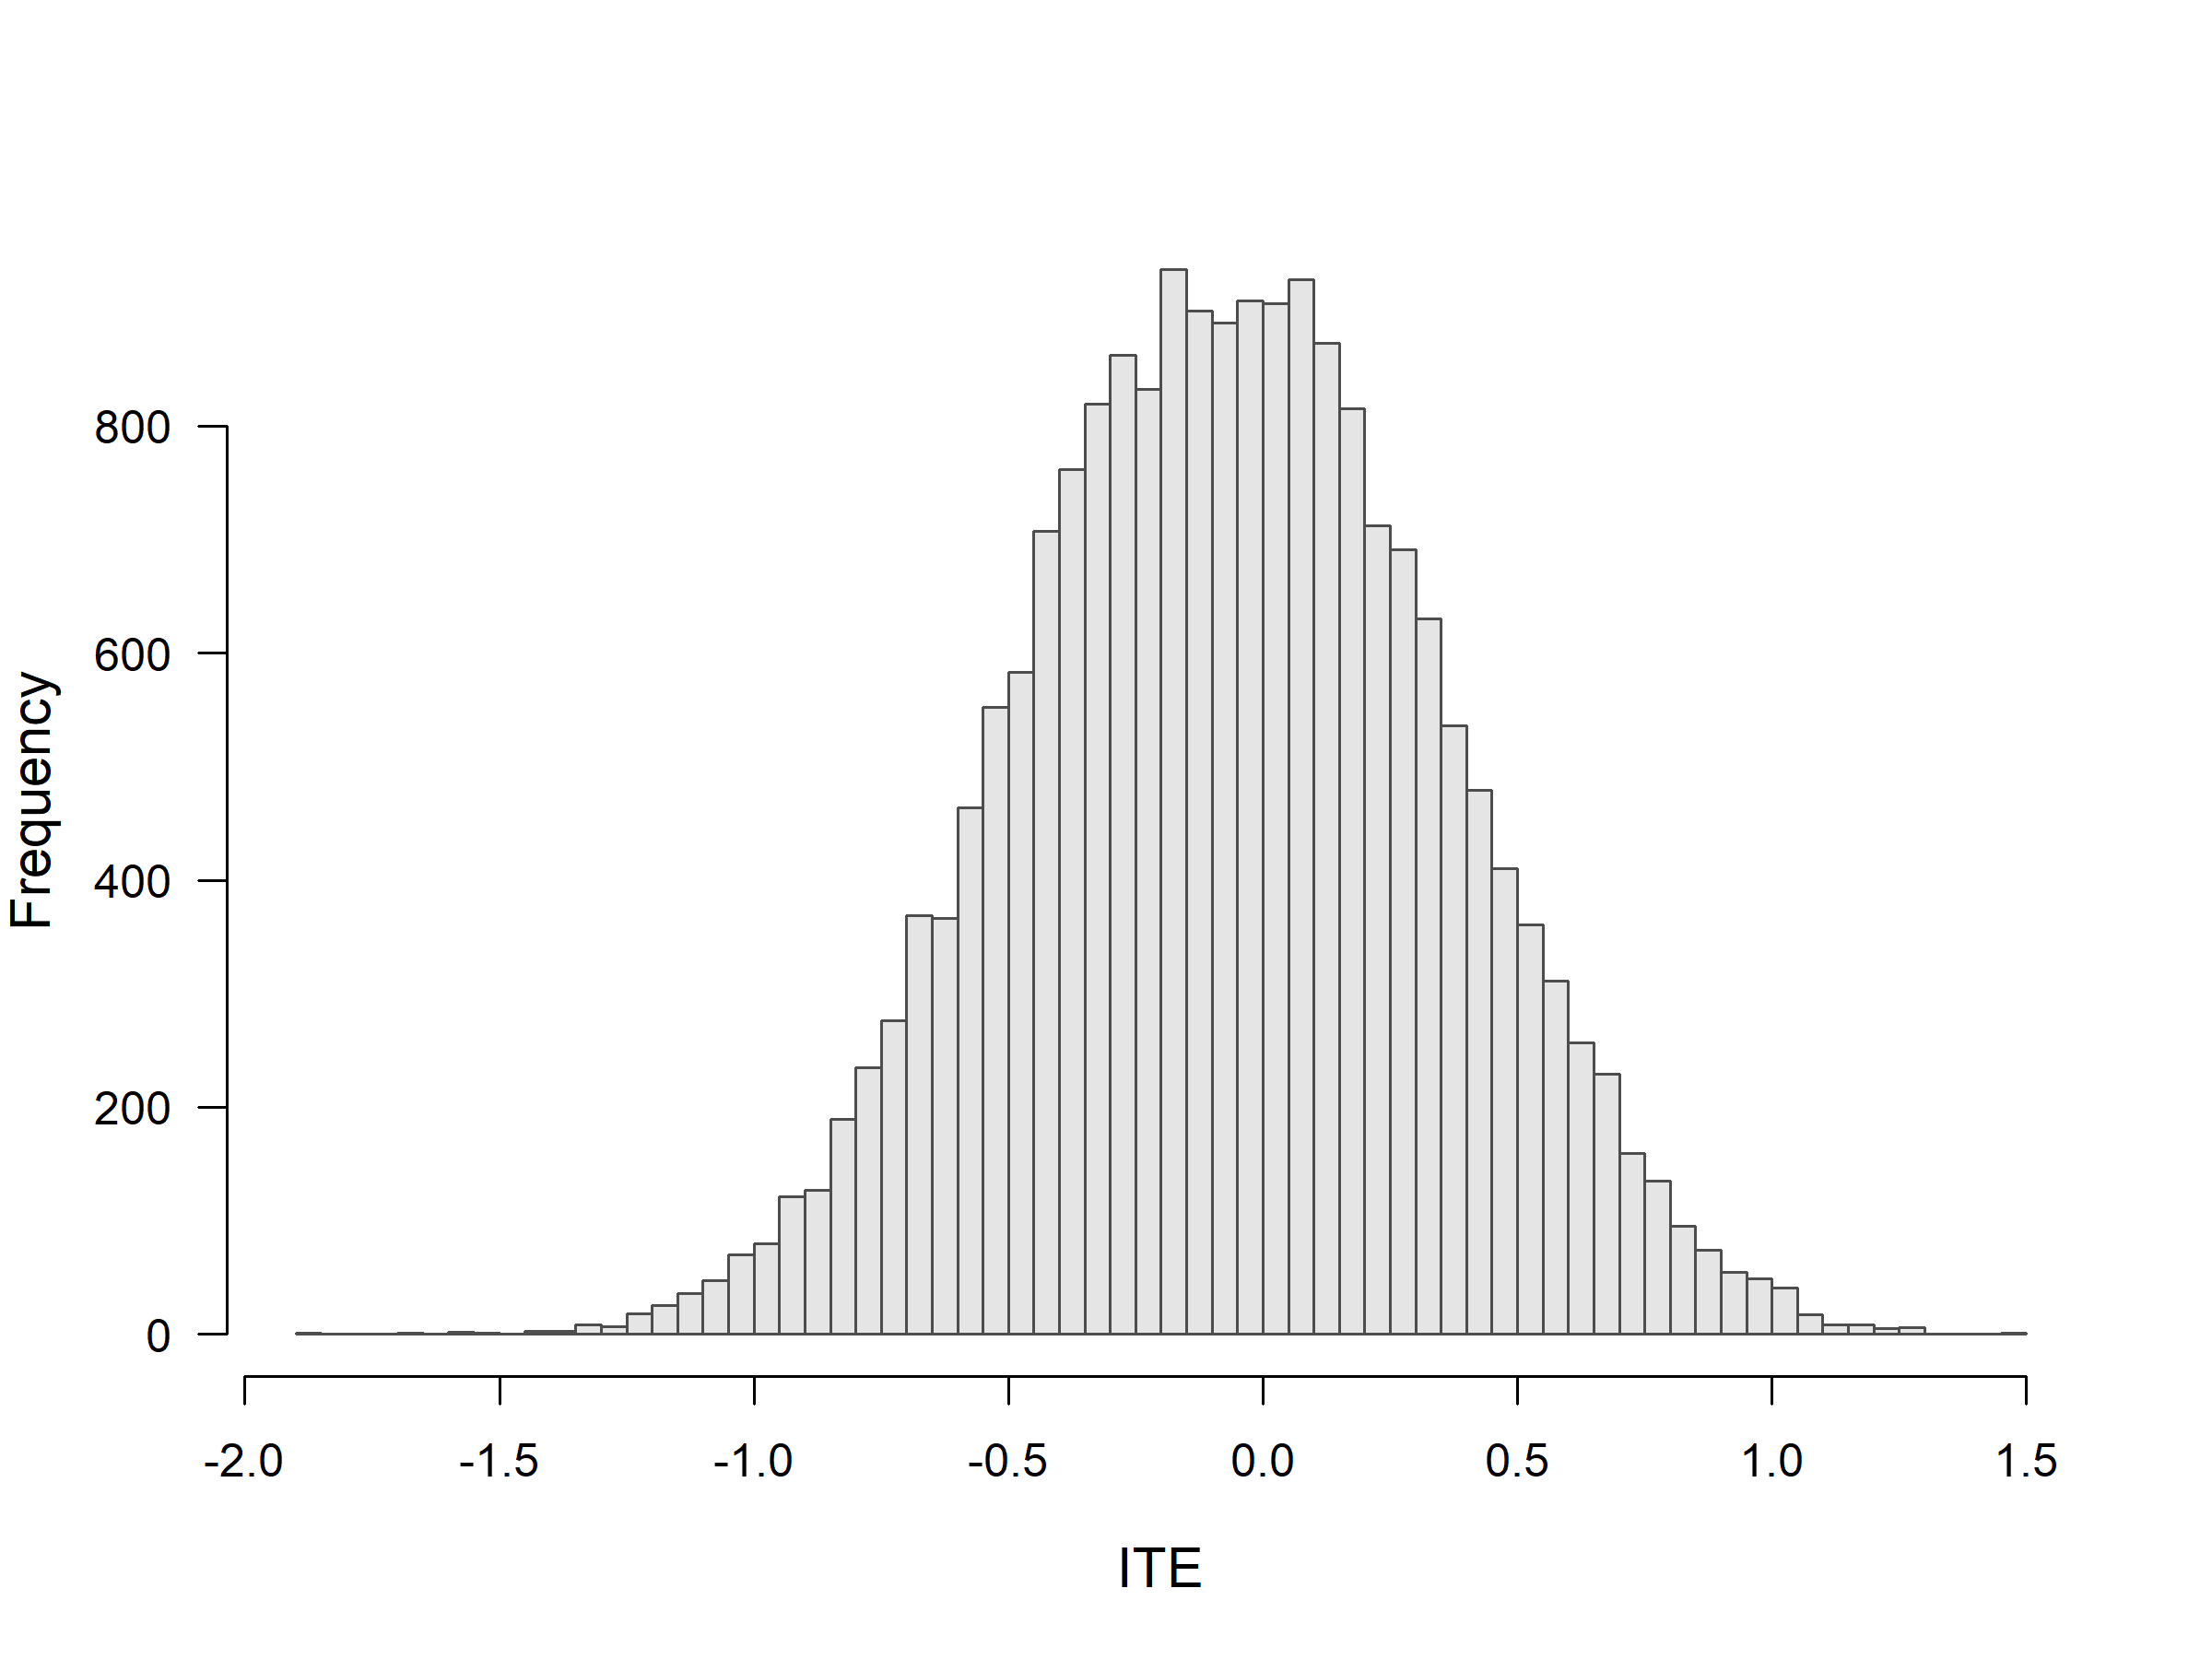
\includegraphics[width=0.7\textwidth]{img/results/observ_scenario3_ite_distribution_dgp.png}
\caption{True ITE distribution resulting from the DGP for Scenario~(3), which includes interaction effects but no direct treatment effect. The true ITEs are identical in the observational and RCT settings, since they are based on the potential outcomes under both treatment allocations. Left: Observational; Right: RCT setting.}
\label{fig:scenario3_ite_distribution_dgp}
\end{figure}



\begin{figure}[htbp]
\centering
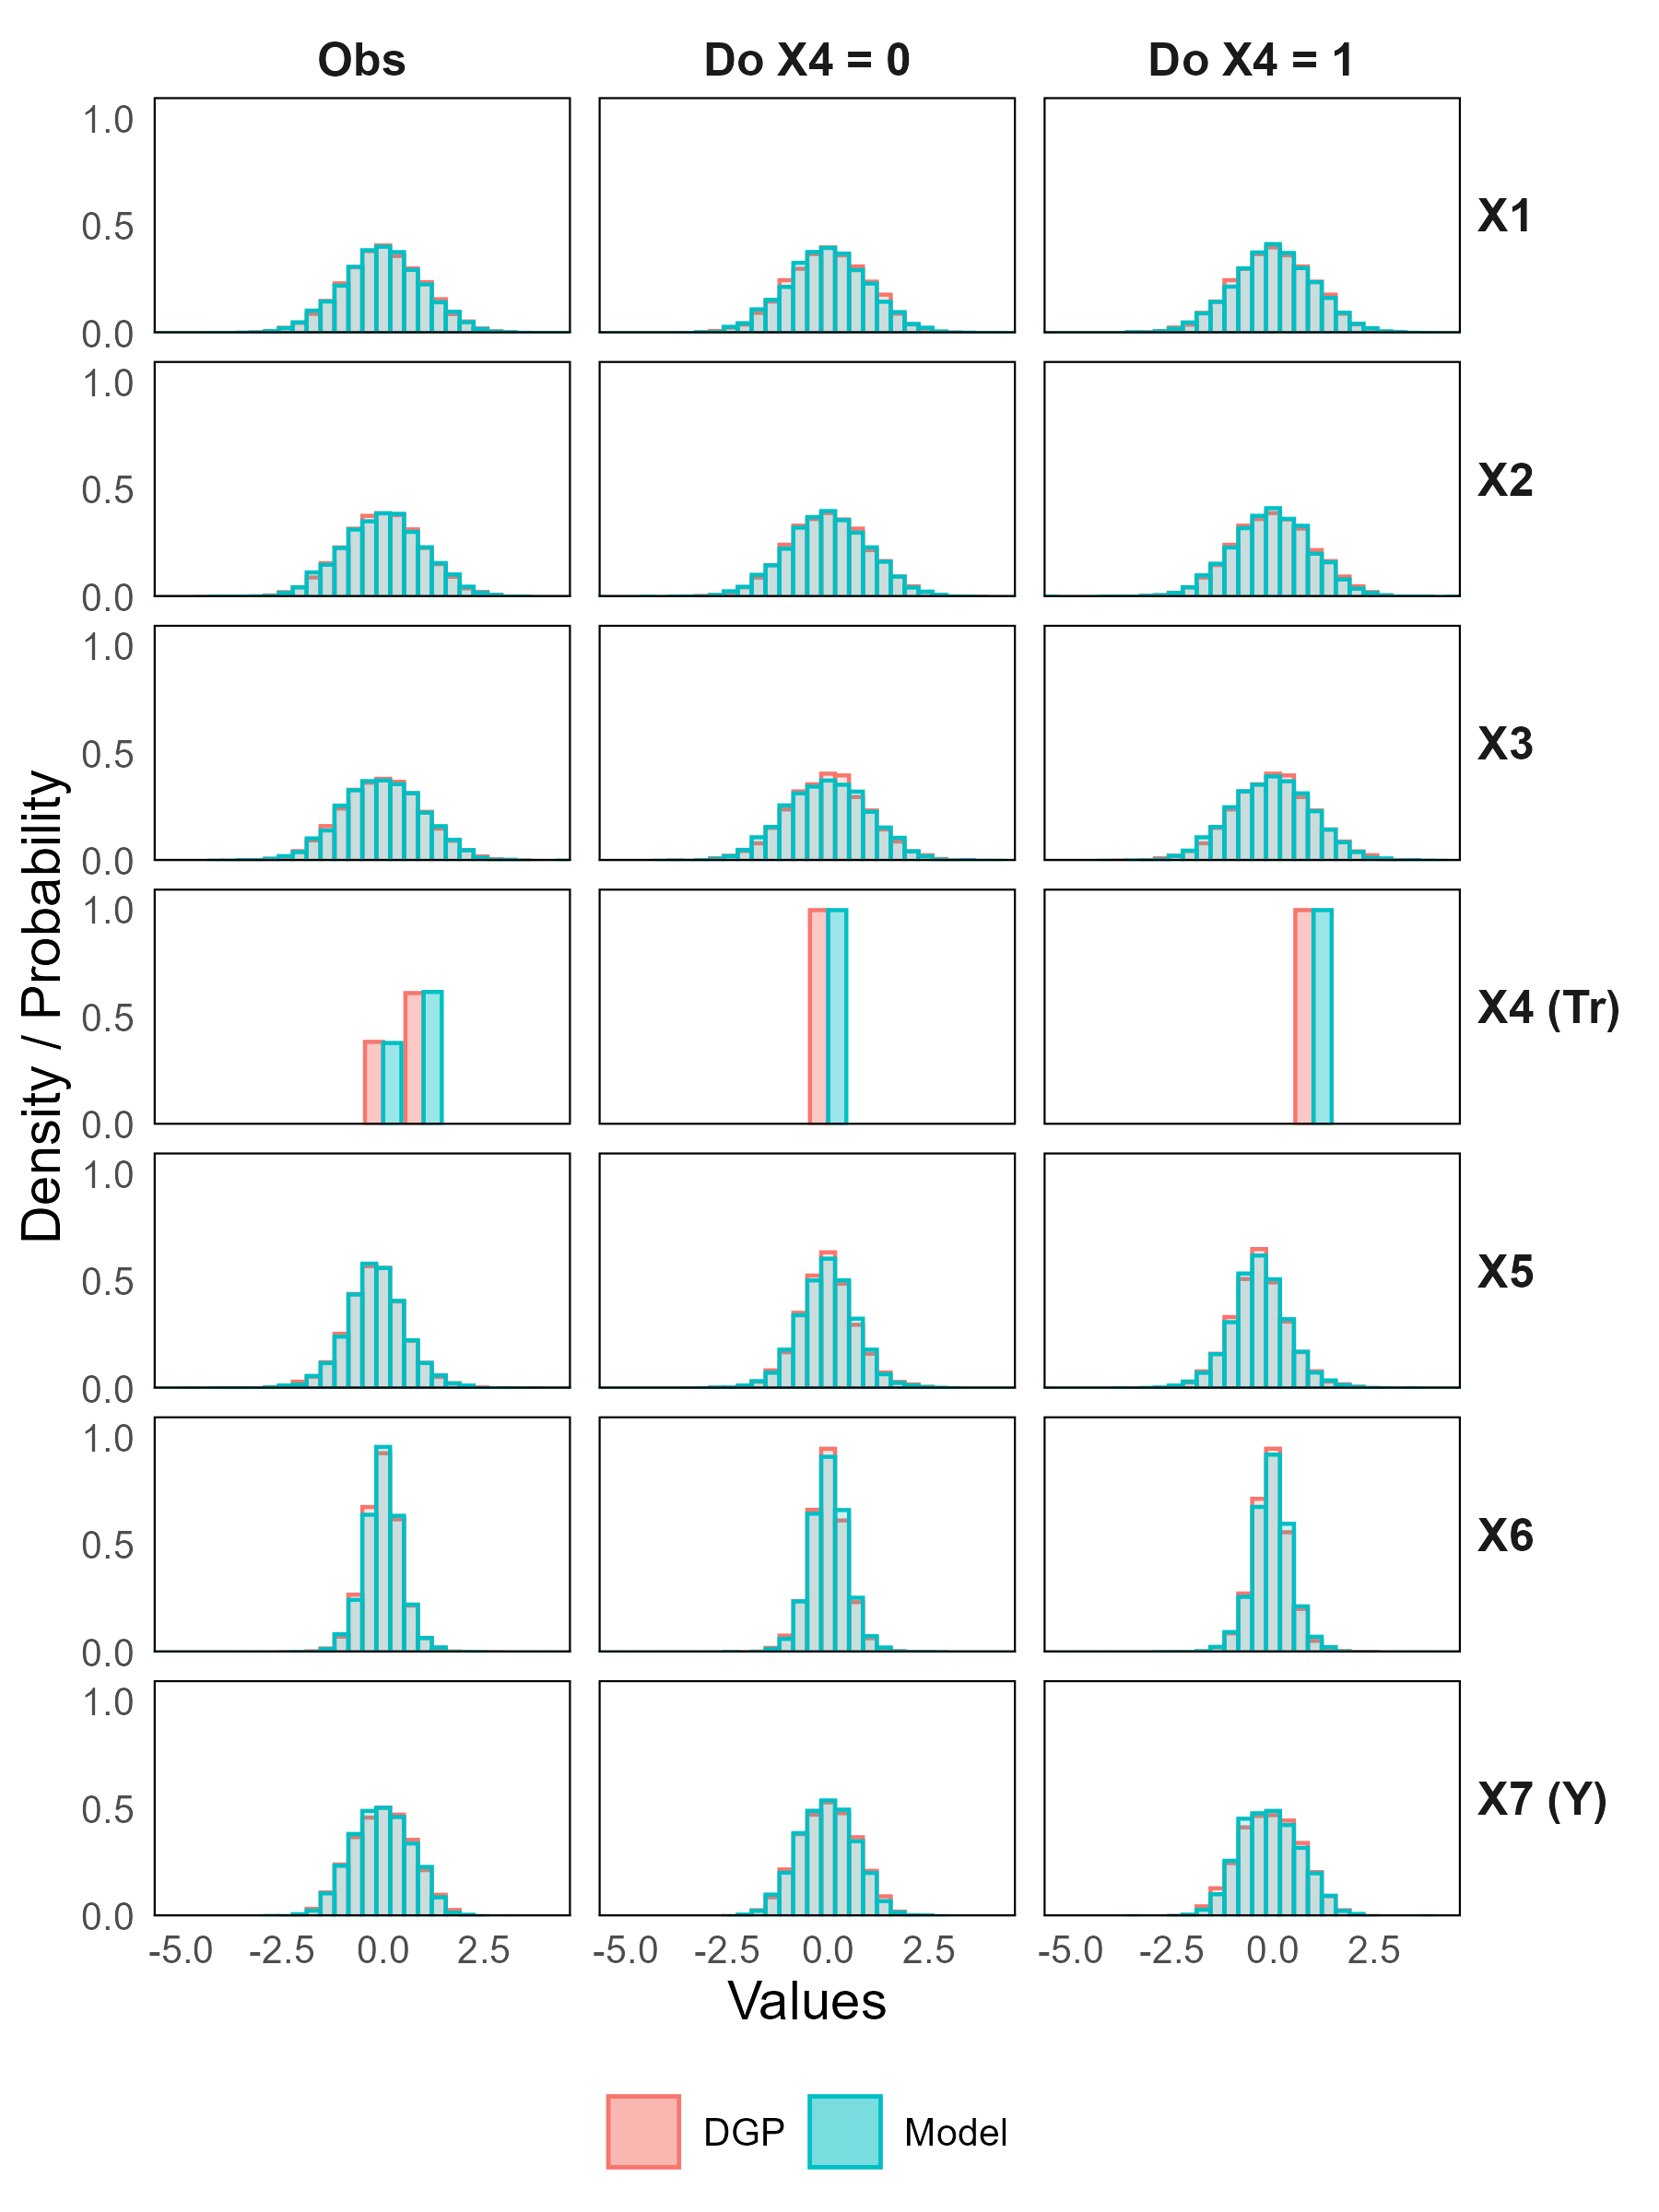
\includegraphics[width=0.45\textwidth]{img/results/observ_scenario3_sampling_distributions_vertical.png}
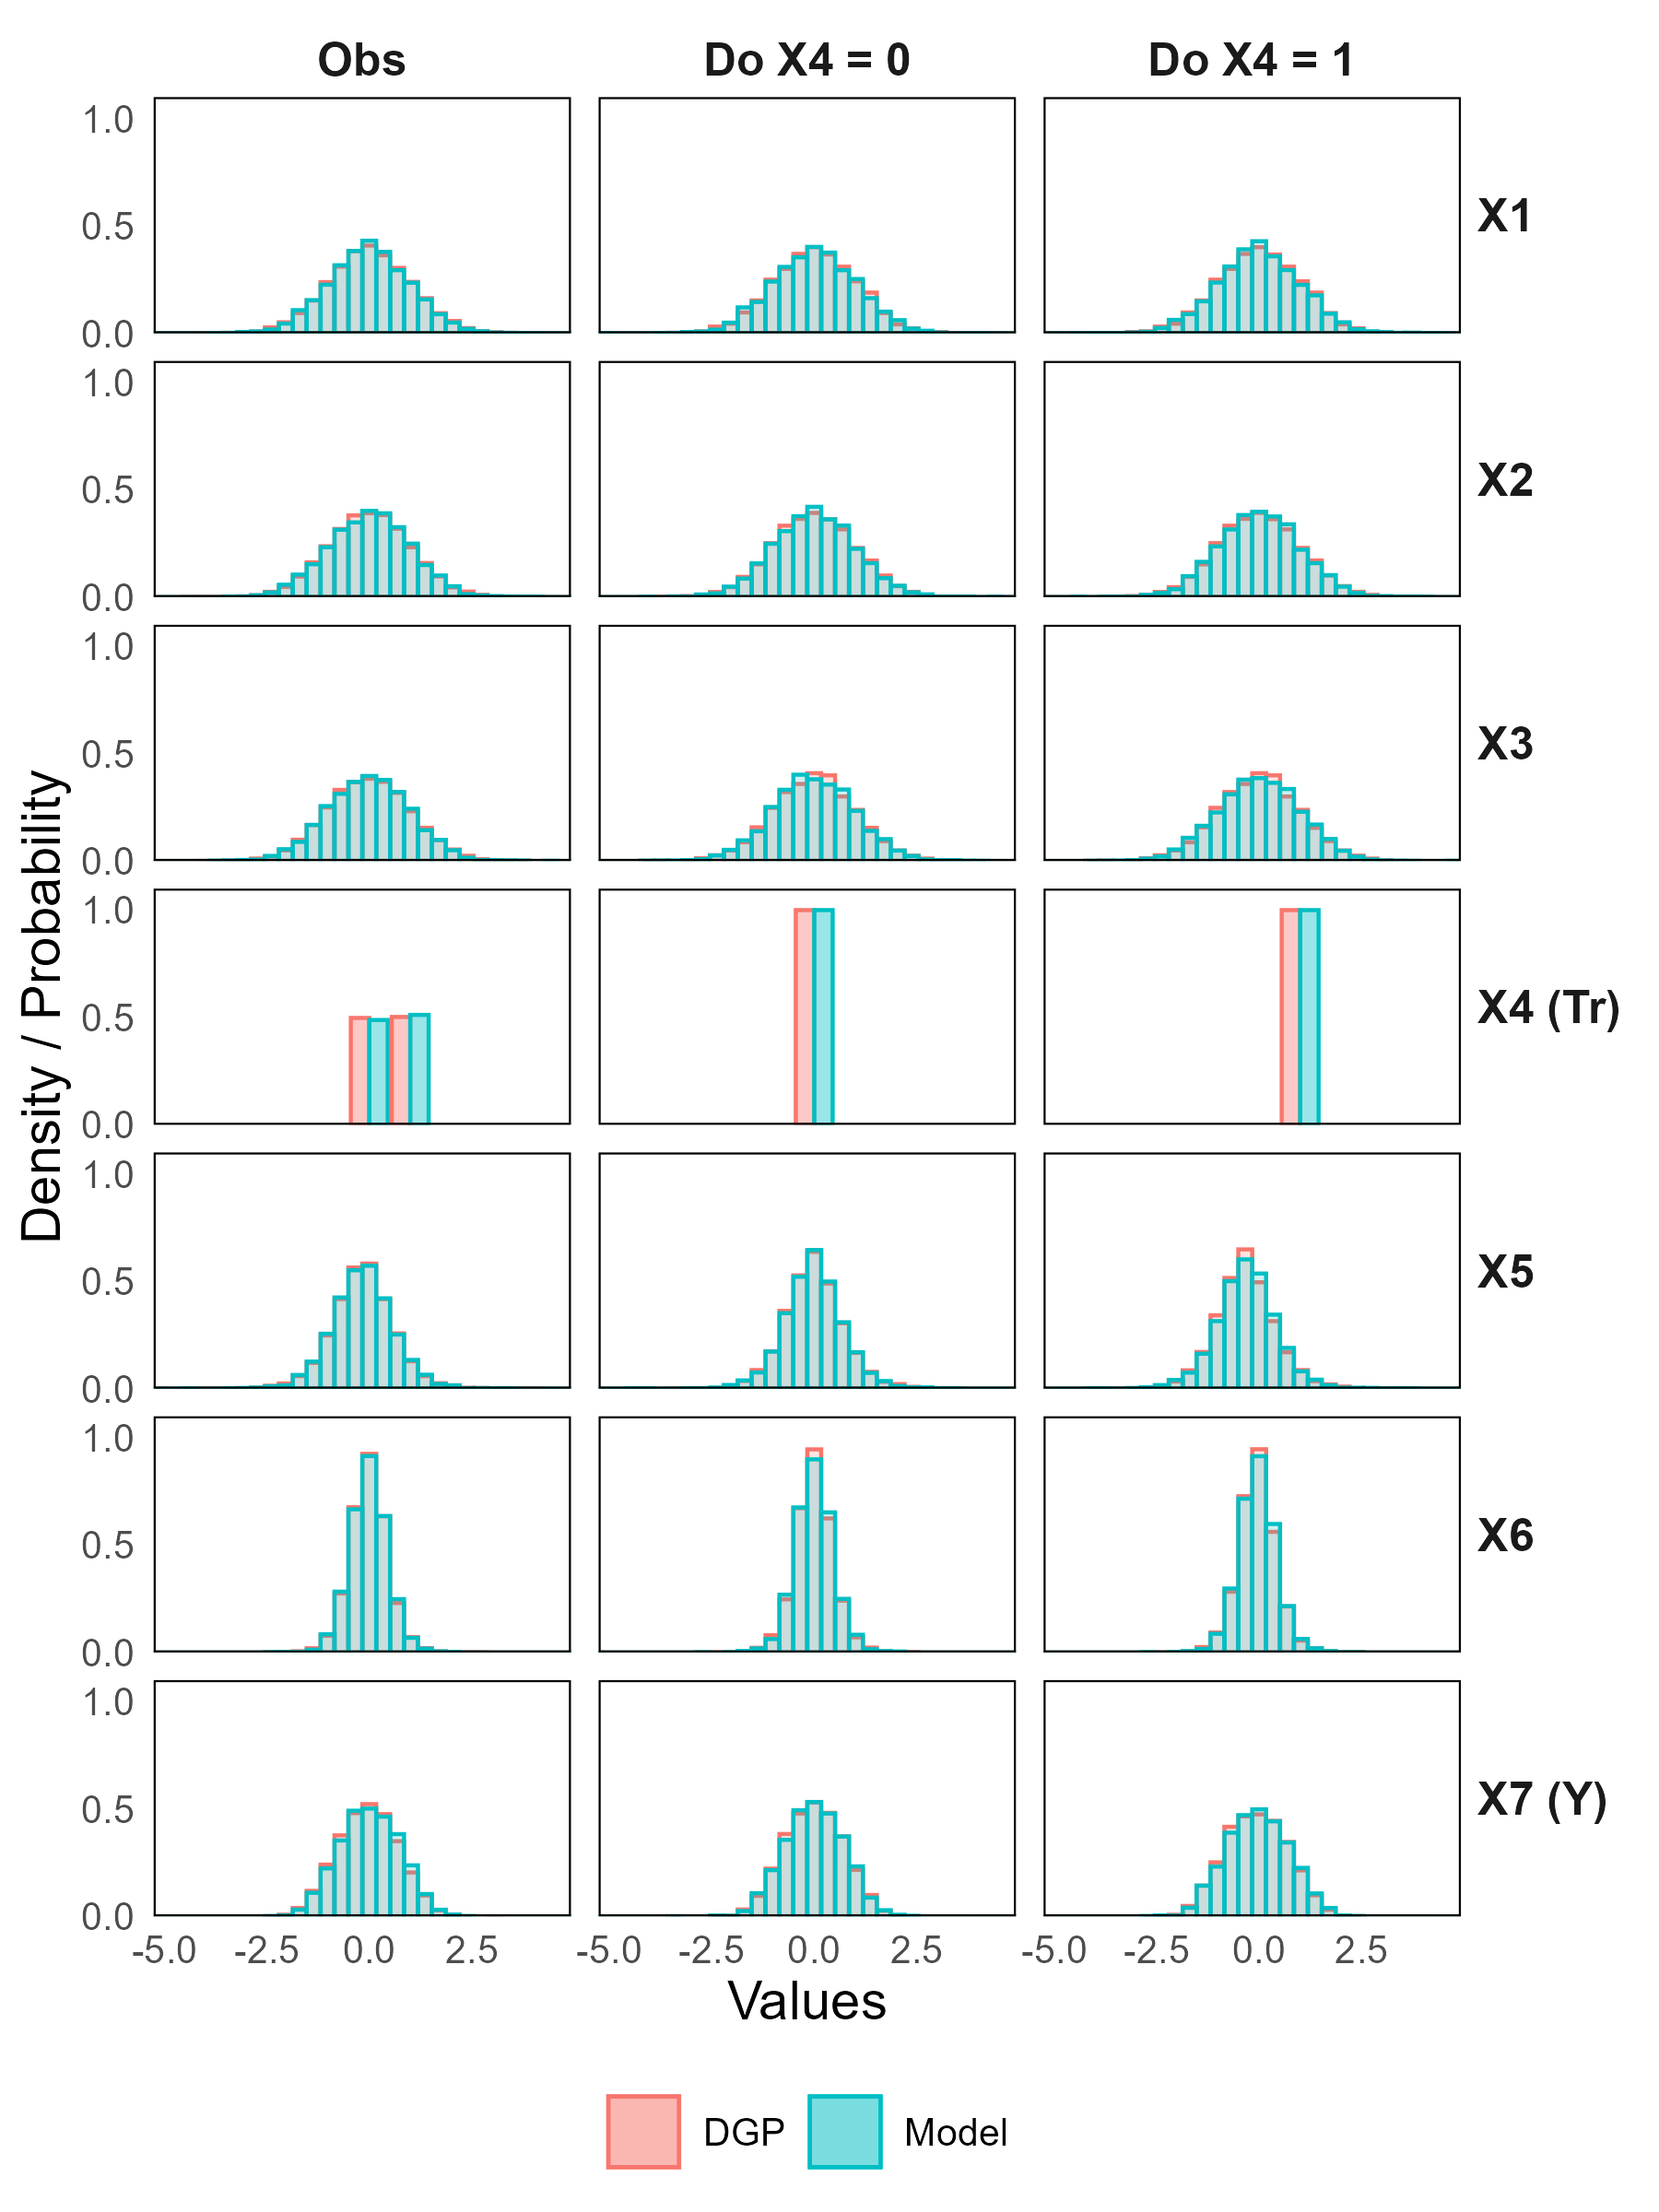
\includegraphics[width=0.45\textwidth]{img/results/rct_scenario3_sampling_distributions_vertical.png}
\caption{Marginal distributions of DGP variables and samples generated by the fitted TRAM-DAG for Scenario~(3), which includes interaction effects but no direct treatment effect. The distributions are shown as observed (Obs), under control intervention (do($X_4 = 0$)), and under treatment intervention (do($X_4 = 1$)). Left: Observational; Right: RCT setting.}
\label{fig:scenario3_sampling_distributions_vertical}
\end{figure}

\begin{figure}[htbp]
\centering
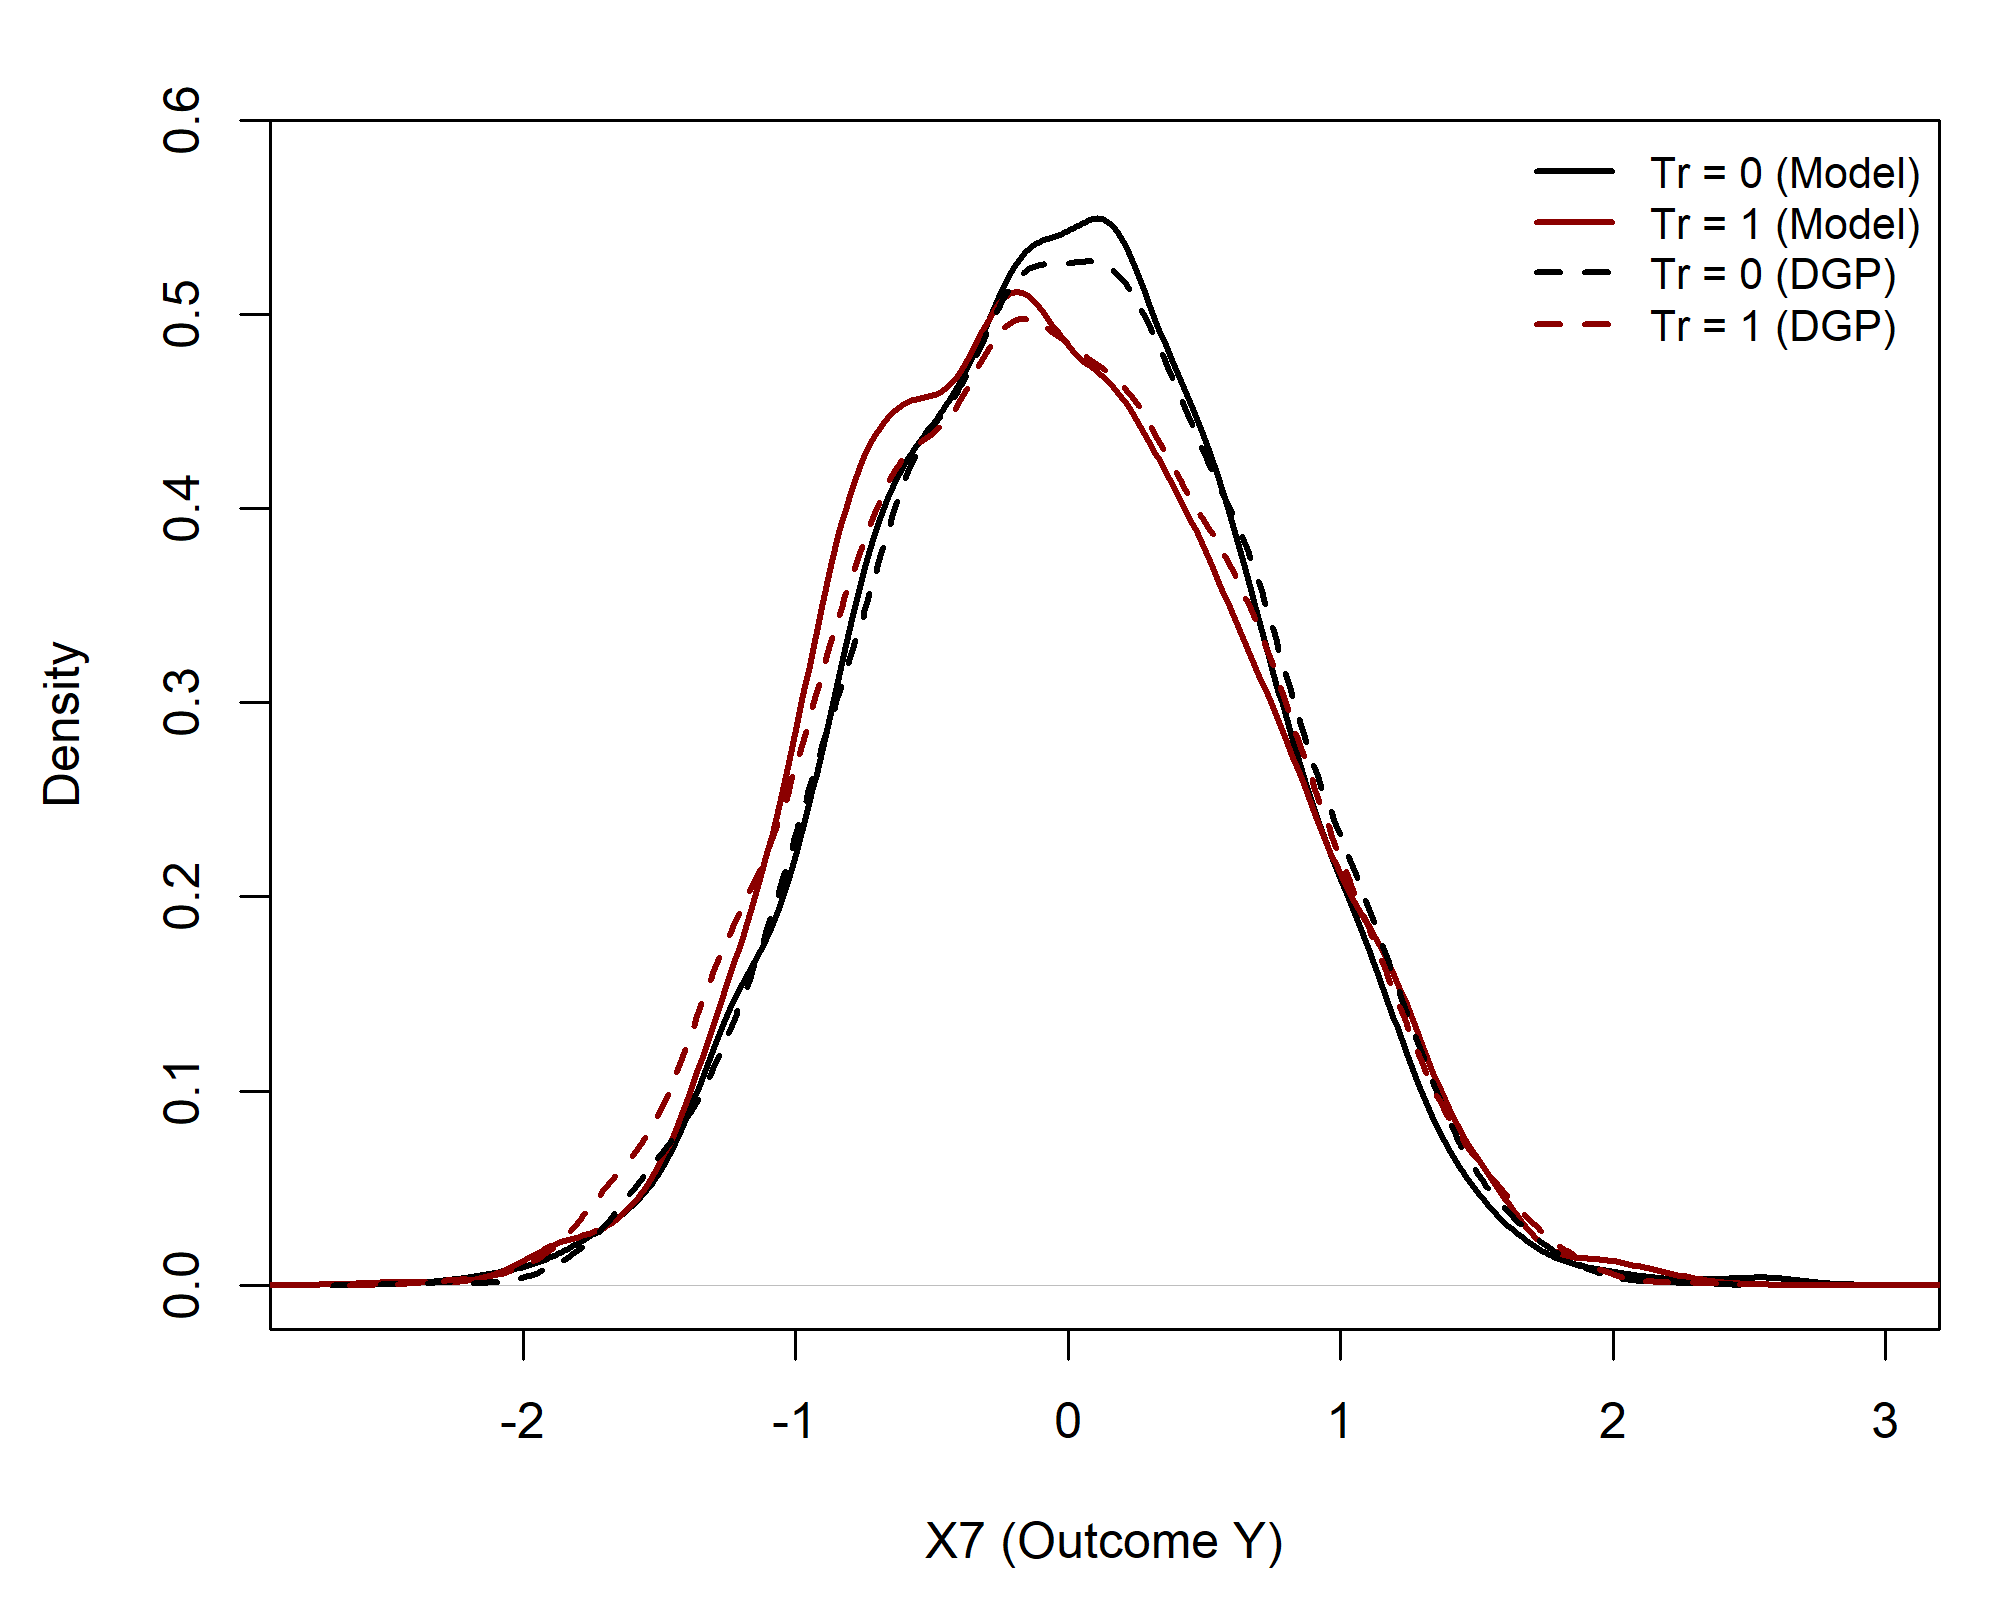
\includegraphics[width=0.45\textwidth]{img/results/observ_scenario3_X7_treatment_densities.png}
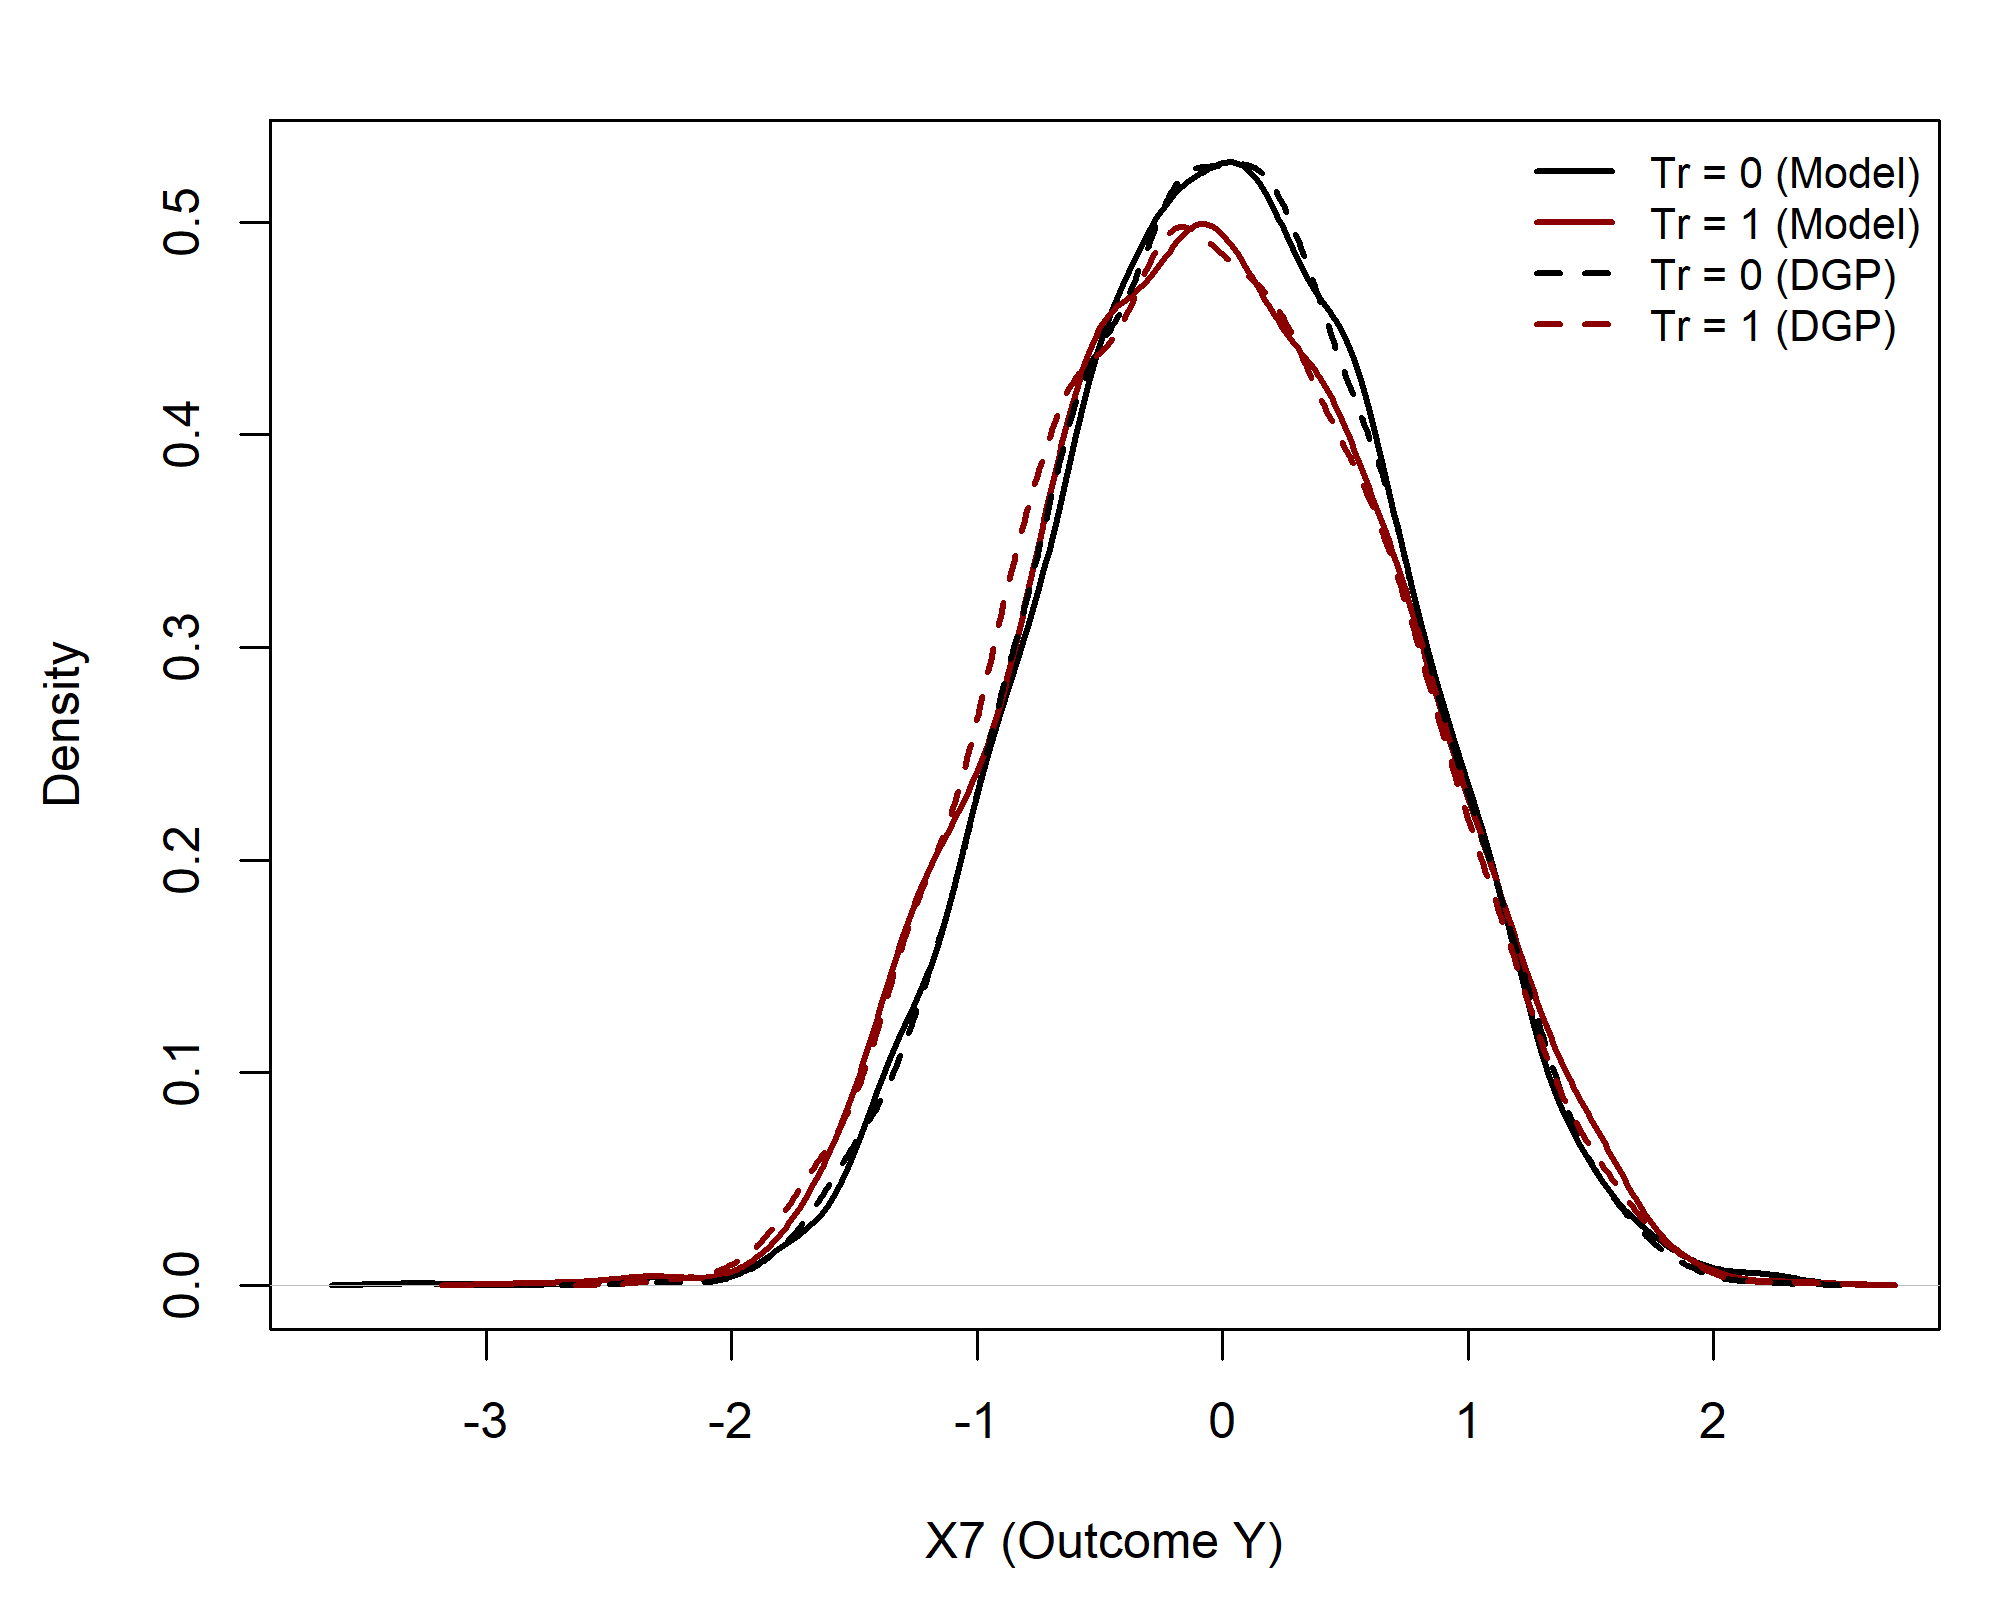
\includegraphics[width=0.45\textwidth]{img/results/rct_scenario3_X7_treatment_densities.png}
\caption{Distributions of the outcome variable ($X_7$) under treatment and control interventions for Scenario~(3), which includes interaction effects but no direct treatment effect. This plot provides a higher resolution view of the $X_7$ panels under do($X_4 = 0$) and do($X_4 = 1$) from Figure~\ref{fig:scenario3_sampling_distributions_vertical}. Left: Observational; Right: RCT setting.}
\label{fig:scenario3_outcome_distributions}
\end{figure}




\begin{figure}[htbp]
\centering
\includegraphics[width=0.33\textwidth]{img/results/observ_scenario3_ITE_densities_train_test.png}
\includegraphics[width=0.33\textwidth]{img/results/rct_scenario3_ITE_densities_train_test.png}
\vspace{-17pt}
\caption{Densities of estimated ITEs compared to the true ITEs in the training and test datasets for Scenario~(3), which includes interaction effects but no direct treatment effect. Left: Observational; Right: RCT setting.}
\label{fig:scenario3_ite_densities_train_test}
\end{figure}






\begin{figure}[htbp]
\centering
\includegraphics[width=0.33\textwidth]{img/results/observ_scenario3_ITE_scatter_train_test.png}
\includegraphics[width=0.33\textwidth]{img/results/rct_scenario3_ITE_scatter_train_test.png}
\vspace{-17pt}
\caption{Scatterplots of estimated ITEs compared to the true ITEs in the training and test datasets for Scenario~(3), which includes interaction effects but no direct treatment effect. Left: Observational; Right: RCT setting.}
\label{fig:scenario3_ite_scatter_train_test}
\end{figure}




\begin{figure}[htbp]
\centering
\includegraphics[width=0.8\textwidth]{img/results/observ_scenario3_ITE_ATE.png}
\vspace{-15pt}
\caption{ITE-ATE plot for Scenario~(3) in the observational setting, which includes interaction effects but no direct treatment effect. Individuals are grouped into bins based on the estimated ITE, and within each bin the ATE is computed as the difference in medians of the observed outcomes under treatment and control. 95\% bootstrap confidence intervals reflect the uncertainty.}
\label{fig:observ_scenario3_ite_ATE}
\end{figure}


\begin{figure}[htbp]
\centering
\includegraphics[width=0.8\textwidth]{img/results/rct_scenario3_ITE_ATE.png}
\vspace{-15pt}
\caption{ITE-ATE plot for Scenario~(3) in the RCT setting, which includes interaction effects but no direct treatment effect. Individuals are grouped into bins based on the estimated ITE, and within each bin the ATE is computed as the difference in medians of the observed outcomes under treatment and control. 95\% bootstrap confidence intervals reflect the uncertainty.}
\label{fig:rct_scenario3_ite_ATE}
\end{figure}


